\documentclass[showframe,11pt,twoside,openright]{report}
\usepackage{standalone}
\standalonetrue
\ifstandalone
  \usepackage{../../haziq_thesis}
  \usepackage{../../haziq_maths}
  \usepackage{../../haziq_glossary}
  \usepackage{../../knitr}
  \usepackage{../../matrix_fig}
  \addbibresource{../../bib/haziq.bib}
  \externaldocument{../01/.texpadtmp/chapter1}
  \externaldocument{../02/.texpadtmp/chapter2}  
  \externaldocument{../03/.texpadtmp/chapter3}
  \externaldocument{../04/.texpadtmp/chapter4}
%  \externaldocument{../05/.texpadtmp/chapter5}
  \externaldocument{../06/.texpadtmp/chapter6}
  \externaldocument{../07/.texpadtmp/chapter7}
  \externaldocument{../appendix/.texpadtmp/appendix}  
\fi

\begin{document}
\hChapterStandalone[5]{I-priors for categorical responses}
\label{chapter5}
\thispagestyle{chapterfive}

\index{categorical response}
Consider polytomous response variables $\by = \{y_1,\dots,y_n\}$, where each $y_i$ takes on exactly one of the values from the set of $m$ possible choices $\{1,\dots,m\}$.
Modelling categorical response variables is of profound interest in statistics, econometrics and machine learning, with applications aplenty. 
In the social sciences, categorical variables often arise from survey responses, and one may be interested in studying correlations between  explanatory variables and the categorical response of interest.
Economists are frequently interested in discrete choice models to explain and predict choices between several alternatives, such as consumers' choices of goods or modes of transport.
In this age of big data, machine learning algorithms are used for classification of observations based on what is usually a large set of variables or features.

The model \cref{eq:model1} subject to normality assumptions \cref{eq:model1ass} is not entirely appropriate for polytomous variables $\by$.
As an extension to the I-prior methodology, we propose a flexible modelling framework suitable for regression of categorical response variables.
In the spirit of generalised linear models \citep{mccullagh1989}, we relate class probabilities of the observations to a normal I-prior regression model via a \emph{link function}.
Perhaps though, it is more intuitive to view it as machine learners do: since the regression function is ranged on the entire real line, it is necessary to ``squash'' it through some sigmoid function to conform it to the interval $[0,1]$ suitable for probability ranges.

Expanding on this idea further, assume that the $y_i$'s follow a categorical distribution \index{distribution!categorical}, $i=1,\dots,n$, denoted by 
\[
  y_i \sim \Cat(p_{i1},\dots,p_{im}),
\]
with the class probabilities satisfying $p_{ij} \geq 0, \forall j=1,\dots,m$ and $\sum_{j=1}^m p_{ij} = 1$. 
The probability mass function (pmf) of $y_i$ is given by
\begin{equation*}%\label{eq:catdist}
  p(y_i) = p_{i1}^{[y_i = 1]} \cdots p_{im}^{[y_i = m]},
\end{equation*}
where the notation $[\cdot]$ refers to the Iverson bracket\footnote{$[A]$ returns 1 if the proposition $A$ is true, and 0 otherwise. The Iverson bracket is a generalisation of the Kronecker delta.}.\index{Iverson bracket} 
As a side note, when there are only two possibilities for each outcome $y_i$, i.e. $m=2$, we have the Bernoulli distribution.
The class probabilities are made to depend on the covariates through the relationship
\begingroup
\setlength{\abovedisplayskip}{9pt}
\setlength{\belowdisplayskip}{8pt}
\[
  g(p_{i1},\dots,p_{im}) = \big(\alpha_1 + f_1(x_i), \dots, \alpha_m + f_m(x_i)\big),
\]
\endgroup
where $g:[0,1]^m\to\bbR^m$ is some specified link function.
As we will see later, an underlying normal regression model as in \cref{eq:model1} subject to \cref{eq:model1ass} naturally implies a \emph{probit} link function.
%, that is, $g$ is the inverse cumulative distribution function (cdf) of a standard normal distribution (or more precisely, a function that \emph{involves} the standard normal cdf).
With an I-prior assumed on the $f_j$'s, we call this method of probit regression using I-priors the \emph{I-probit} regression model.

%Implicitly in the above, there are $m$ regression curves which model the $m$ class probabilities.
%Often times, it is of interest that the model captures the correlations between choices, which are vital in choice models.
%Disregarding the correlations violates the independence of irrelevant alternatives (IIA) assumption, but this is usually fine for classification tasks where the alternatives are assumed not to be correlated.

Due to the nature of the model assumptions, unfortunately the posterior distribution of the regression functions cannot be found in closed form.
In particular, marginalising the I-prior from the joint likelihood involves a high-dimensional intractable integral (c.f. {\color{\mycitecolour}Equation}\ref{eq:intractablelikelihood2}).
Similar problems are encountered in mixed logistic or probit multinomial models \citep{breslow1993approximate,mcculloch2000bayesian} and also in Gaussian process classification \citep{neal1999,rasmussen2006gaussian}.
In these models, Laplace approximation for maximum likelihood (ML) estimation or Markov chain Monte Carlo (MCMC) methods for Bayesian estimation are used. \index{logistic}
We instead explore a \emph{variational approximation} to the marginal log-likelihood, and by extension, to the posterior density of the regression functions.
The main idea is to replace the difficult posterior distribution with an approximation that is tractable to be used within an EM framework.
As such, the computational work derived in the previous section is applicable for the estimation of I-probit models as well.

As in the normal I-prior model, the I-probit model estimated using a \emph{variational EM algorithm} is seen as an empirical Bayes method of estimation, since the model parameters are replaced with their (pseudo) ML estimates.
It is emphasised again, that working in such a semi-Bayesian framework allows fast estimation of the model in comparison to traditional MCMC, yet provides us with the conveniences that come with Bayesian machinery.
For example, inferences around log odds is usually cumbersome for probit models, but a credibility interval can easily be obtained by resampling methods from the posterior distribution of the regression function, which, as we shall see, is approximated to be normally distributed.

By choosing appropriate RKHSs/RKKSs for the regression functions, we are able to fit a multitude of binary and multinomial models, including multilevel or random-effects models, linear and non-linear classification models, and even spatio-temporal models.
Examples of these models applied to real-world data is shown in  \cref{sec:iprobiteg}.
We find that the many advantages of the normal I-prior methodology  transfer over quite well to the I-probit model for binary and multinomial regression.

%\section{A naïve model}\label{sec:iprobitnaive}
%\index{classification!naive@naïve}
We describe a naïve classification model using I-priors.
Here, the responses are categorical $y_i \in \{ 1,\dots,m \} =: \cM$, and additionally, write $\by_{i \bigcdot} = (y_{i1},\dots,y_{im})^\top$ where the class responses $y_{ij}$ equal one if individual $i$'s response category is $y_i = j$, and zero otherwise.
In other words, there is exactly a single `1' at the $j$'th position in the vector $\by_{i \bigcdot}$, and zeroes everywhere else.
For $j=1,\dots,m$, we model 
\begin{equation}\label{eq:naiveclassmod}
  \begin{gathered}
    y_{ij} = \alpha + 
    \myoverbrace{\alpha_j + f_j(x_i)}{f(x_i,j)}
    + \epsilon_{ij}  \\
    (\epsilon_{i1},\dots,\epsilon_{im})^\top \iid \N_m(\bzero,\bPsi^{-1}).
  \end{gathered}
\end{equation}
The idea here is to model the class responses $y_{ij}$ using class-specific regression functions, in which class responses are assumed to be independent among individuals, but may or may not be correlated among classes for each individual.
The class correlations manifest themselves in the variance of the errors $\bPsi^{-1}$, which is an $m\times m$ matrix.

\index{ANOVA!kernel/RKKS|)}
Denote the regression function $f$ in \cref{eq:naiveclassmod} on the set $\cX\times\cM$ as $f(x_i,j) = \alpha_j + f_j(x_i)$.
This regression function corresponds to an ANOVA decomposition of the spaces $\cF_\cM$ and $\cF_\cX$ of functions over $\cM$ and $\cX$ respectively. 
That is, $\cF = \cF_\cM \oplus (\cF_\cM \otimes \cF_\cX)$ is a decomposition into the main effects of class, and an interaction effect of the covariates for each class.
Let $\cF_\cM$ and $\cF_\cX$ be RKHSs respectively with kernels $a:\cM\times\cM\to\bbR$ and $b_\eta:\cX\times\cX\to\bbR$.
Then, the ANOVA RKKS $\cF$ possesses the reproducing kernel $h_\eta:(\cX \times \cM)^2 \to \bbR$ as defined by
\begin{align}\label{eq:anovaclass}
  h_\eta\big( (x,j), (x',j') \big) = a(j,j') + a(j,j')b_\eta(x,x'), 
\end{align}
which leaves the $\alpha$ to be estimated separately (see \cref{sec:intercept}).
The kernel $b_\eta$ may be any of the kernels described in this thesis, ranging from the linear kernel, to the fBm kernel, or even an ANOVA kernel.
Choices for $a:\cM \times \cM \to \bbR$ include \index{Pearson kernel/RKHS} \index{identity kernel}
\begin{enumerate}
  \item \textbf{The Pearson kernel} (as defined in \cref{def:pearson}, \mypageref{def:pearson}). With $J\sim\Prob$, a probability measure over $\cM$,
  \[
    a(j,j') = \frac{\delta_{jj'}}{\Prob(J=j)} - 1.
  \]
  \item \textbf{The centred identity kernel}. With $\delta$ denoting the Kronecker delta function,
  \[
    a(j,j') = \delta_{jj'} - 1 / m.
  \]
\end{enumerate}
The purpose of either of these kernels is to contribute to the class intercepts $\alpha_j$, and to associate a regression function in each class.
The only difference between the two is the inverse probability weighting per class that is applied in the Pearson kernel, but not in the identity kernel.

With $f \in \cF$ (the RKKS with kernel $h_\eta$), it is straightforward to assign an I-prior on $f$. 
It is in fact
\begin{align}\label{eq:naiveclassiprior}
  \begin{gathered}
    f(x_i,j) = \sum_{j'=1}^m\sum_{i'=1}^n a(j,j')\big(1 + b_\eta(x_i,x_{i'})\big) w_{i'j'} \\
    (w_{i'1},\dots,w_{i'm})^\top \iid \N_m(\bzero,\bPsi)
  \end{gathered}
\end{align}
assuming a zero prior mean $f_0(x,j) = 0$.
The model then classifies the $i$'th data point to class $j$ if $\hat y_{ij} = \max(\hat y_{i1},\dots,\hat y_{im})$, where $\hat y_{ik} = \hat\alpha + \hat f(x_i,k)$, the prediction for the $k$'th component of $y_i$.

There are several drawbacks to using the model described above.
Unlike in the case of continuous response variables, the normal I-prior model is highly inappropriate for categorical responses.
For one, it violates the normality and homoscedasticity assumptions of the errors.
For another, predicted values may be out of the range $[0,m]$ and thus poorly calibrated.
Furthermore, it would be more suitable if the class probabilities---the probability of an observation belonging to a particular class---were also part of the model.
In \cref{chapter5}, we propose an improvement to this naïve I-prior classification model by considering a probit-like transformation of the regression functions.

%\begin{proof}
%  \[
%    f(x_i,j) = \sum_{j'=1}^m\sum_{i'=1}^n a(j,j')\big(1 + b_\eta(x_i,x_{i'})\big) w_{i'j'}
%  \]
%  
%  \[
%    \alpha_j = \sum_{j'=1}^m\sum_{i'=1}^n a(j,j') w_{i'j'}
%  \]
%  
%  \begin{align*}
%    \sum_{j=1}^m \alpha_j
%    &= \sum_{j=1}^m \sum_{j'=1}^m\sum_{i'=1}^n a(j,j') w_{i'j'} \\
%    &= \sum_{j=1}^m \sum_{j'=1}^m\sum_{i'=1}^n \delta_{jj'} w_{i'j'} \\
%    &= \sum_{j=1}^m\sum_{i'=1}^n  w_{i'j}
%  \end{align*}
%  
%  \begin{align*}
%    \sum_{j=1}^m f_j(x_i)
%    &= \sum_{j=1}^m \sum_{j'=1}^m\sum_{i'=1}^n a(j,j')b_\eta(x_i,x_{i'}) w_{i'j'} \\
%    &= \sum_{j=1}^m \sum_{j'=1}^m\sum_{i'=1}^n \delta_{jj'} b_\eta(x_i,x_{i'}) w_{i'j'} \\
%    &= \sum_{j=1}^m\sum_{i'=1}^n b_\eta(x_i,x_{i'}) w_{i'j}
%  \end{align*}
%  
%  \begin{align*}
%    \sum_{i=1}^n f_j(x_i)
%    &= \sum_{i=1}^n \sum_{j'=1}^m\sum_{i'=1}^n a(j,j')b_\eta(x_i,x_{i'}) w_{i'j'} \\
%    &= \sum_{i=1}^n \sum_{j'=1}^m\sum_{i'=1}^n \delta_{jj'} b_\eta(x_i,x_{i'}) w_{i'j'} 
%  \end{align*}
%\end{proof}

%Rearrange the $n$ observations per class.
%Let $\bff_j = \big(f_j(x_1),\dots,f_j(x_n)\big)^\top \in \bbR^n$.
%We can write the I-prior as $\bff_j = \bA_{jj} \cdot \bH\bw_j$
%Therefore, $\bff_j \sim \N_n(\bzero, \bPsi_{jj}\bA_{jj} \bH^2)$, and
%\begin{align*}
%  \Cov(\bff_j,\bff_k) &= \Cov(\bA_{jj} \cdot \bH\bw_j, \bA_{kk} \cdot \bH\bw_k) \\
%  &= \bA_{jj}\bA_{kk} \cdot \bH \Cov(\bw_j,\bw_k) \bH \\
%  &= \bA_{jj}\bA_{kk}\bPsi_{jk} \bH^2.
%\end{align*}


\section{A latent variable motivation: the I-probit model}\label{sec:iprobitlatentvarmot}
It is convenient, as we did in \hltodo{Section X naive classification}, to again think of the responses $y_i \in \{1,\dots,m\} = \cM$ as comprising of a binary vector $\by_{i \bigcdot} = (y_{i1},\dots,y_{im})^\top$, with a single `1' at the position corresponding to the value that $y_i$ takes. 
That is,
\[
  y_{ik} =
  \begin{cases}
    1 &\text{ if } y_i = k \\
    0 &\text{ if } y_i \neq k.
  \end{cases}
\]
With $y_i\iid\Cat(p_{i1},\dots,p_{im})$ for $i=1,\dots,n$, each $y_{ij}$ is distributed as Bernoulli with probability $p_{ij}$, $j=1,\dots,m$ according to the above formulation. 
Now, assume that, for each $y_{i1}, \dots, y_{im}$, there exists corresponding \emph{continuous, underlying, latent variables} $y_{i1}^*, \dots, y_{im}^*$ such that
\begin{align}\label{eq:latentmodel}
  y_i =
  \begin{cases}
    1 &\text{ if } y_{i1}^* \geq y_{i2}^*, y_{i3}^*, \dots, y_{im}^* \\
    2 &\text{ if } y_{i2}^* \geq y_{i1}^*, y_{i3}^*, \dots, y_{im}^* \\
    \,\vdots \\
    m &\text{ if } y_{im}^* \geq y_{i2}^*, y_{i3}^*, \dots, y_{i\,m-1}^*. \\
  \end{cases}  
\end{align}
In other words, 
%$y_{ij} = [y_{ij}^* = \max_k y_{ik}^*]$.
$y_{ij} = \argmax_{k=1}^m y_{ik}^*$.
Such a formulation is common in economic choice models, and is rationalised by a utility-maximisation argument: an agent faced with a choice from a set of alternatives will choose the one which benefits them most.
In this sense, the $y_{ij}^*$'s represent individual $i$'s \emph{latent propensities} for choosing alternative $j$.

Instead of modelling the observed $y_{ij}$'s directly, we model instead the $n$ latent variables in each class $j=1,\dots,m$ according to the regression problem
\begin{equation}\label{eq:multinomial-latent}
  \begin{gathered}
    y_{ij}^* = \alpha + \alpha_j + f_j(x_i) + \epsilon_{ij} \\
    (\epsilon_{i1}, \dots, \epsilon_{im})^\top  \iid \N_m(\bzero, \bPsi^{-1}). 
  \end{gathered}
\end{equation}
%with $\alpha_j$ being an intercept, and $f_j:\cX \to \bbR$ a regression function belonging to some RKHS/RKKS of functions $\cF$.
%having the reproducing kernel $h_{\eta_j}: \cX \times \cX \to \bbR$. 
We can see some semblance of this model with the one in \cref{eq:naiveclassiprior}, and ultimately the aim is to assign I-priors to the regression function of these latent variables, which we shall describe shortly.
For now, write $\bmu(x_i) \in \bbR^m$ whose $j$'th component is $\alpha + \alpha_j + f_j(x_i)$, and realise that each $\by_{i \bigcdot}^* = (y_{i1}^*, \dots, y_{im}^*)^\top$ has the distribution $\N_m(\bmu(x_i), \bPsi^{-1})$, conditional on the data $x_i$,  the intercepts $\alpha,\alpha_1,\dots,\alpha_m$, the evaluations of the functions at $x_i$ for each class $f_1(x_i), \dots, f_m(x_i)$, and the error covariance matrix $\bPsi^{-1}$.

\newcommand{\intset}{\{y_{ij}^* > y_{ik}^* \,|\, \forall k \neq j\}}
The probability $p_{ij}$ of observation $i$ belonging to class $j$ is calculated as 
\begin{align}
  p_{ij} 
  &= \Prob(y_i = j) \nonumber \\
  &= \Prob\big(\intset\big) \nonumber \\
  &= \idotsint\displaylimits_{\intset} \phi(y_{i1}^*, \dots, y_{im}^*|\bmu(x_i), \bPsi^{-1}) \dint y_{i1}^* \cdots \dint y_{im}^*,\label{eq:pij}
%  =: g_{j}^{-1} ( \bmu(x_i) | \bPsi ),
\end{align}
where $\phi(\cdot|\mu,\Sigma)$ is the density of the multivariate normal with mean $\mu$ and variance $\Sigma$.
This is the probability that the normal random variable $\by_{i \bigcdot}^*$ belongs to the set $\cC_j := \intset$, which are cones in $\bbR^m$.
Since the union of these cones is the entire $m$-dimensional space of reals, the probabilities add up to one and hence they represent a proper probability mass function for the classes.
%Upon knowing all values for $\alpha_j$, $f_j(x_i)$, and $\bSigma$, one is able to calculate $p_{ij}$ through the relationship \eqref{eq:pij}, which we denote as $g^{-1}$.
While this does not have a closed-form expression and highlights one of the difficulties of working with probit models, the integral is by no means impossible to compute---see \cref{sec:mnint} for a note regarding this matter.


Now, we'll see how to specify an I-prior on the regression problem \cref{eq:multinomial-latent}.
In the naïve I-prior model, we wrote $f(x_i,j) = \alpha_j + f_j(x_i)$, and called for $f$ to belong to an ANOVA RKKS with kernel defined in \cref{eq:anovaclass}.
Instead of doing the same, we take a different approach.
Treat the $\alpha_j$'s in \cref{eq:multinomial-latent} as intercept parameters to estimate with the additional requirement that $\sum_{j=1}^m \alpha_j = 0$.
Further, let $\cF$ be a (centred) RKHS/RKKS of functions over $\cX$ with reproducing kernel $h_\eta$.
Now, consider putting an I-prior on the regression functions $f_j \in \cF$, $j=1\dots,m$, defined by
\[
  f_j(x_i) = f_0(x_i,j) + \sum_{k=1}^n h_\eta(x_i,x_k)w_{ik}
\]
with $\bw_{i \bigcdot} := (w_{i1},\dots,w_{im})^\top \iid \N(0,\bPsi)$.
This is similar to the naïve I-prior specification \cref{eq:naiveclassiprior}, except that the intercept  have been treated as parameters rather than accounting for them using an RKHS of functions (Pearson RKHS or identity kernel RKHS).
Importantly, the overall regression relationship still satisfies the ANOVA functional decomposition, because the $\alpha_j$'s sum to zero.
We find that this approach bodes well down the line computationally.

We call the multinomial probit regression model of \cref{eq:latentmodel} subject to \cref{eq:multinomial-latent} and I-priors on $f_j \in \cF$, the \emph{I-probit model}.
For completeness, this is stated again: for $i=1,\dots,n$, $y_i = \argmax_{k=1}^m y_{ik}^* \in \{1,\dots,m\}$, where, for $j=1,\dots,m$,
\begin{align}\label{eq:iprobitmod}
  \begin{gathered}
    y_{ij}^* = \alpha + \alpha_j + 
    \greyoverbrace{f_0(x_i, j) + \sum_{k=1}^n h_\eta(x_i,x_k)w_{ik}}{f_j(x_i)}
    + \epsilon_{ij} \\
    \bepsilon_{i \bigcdot} := (\epsilon_{i1}, \dots, \epsilon_{im})^\top  \iid \N_m(\bzero, \bPsi^{-1}) \\
    \bw_{i \bigcdot} := (w_{i1},\dots,w_{im})^\top \iid \N_m(\bzero,\bPsi).
  \end{gathered}
\end{align}
The parameters of the I-probit model are denoted by $\theta = \{\alpha_1,\dots,\alpha_m,\eta,\bPsi \}$.
To establish notation, let 
\begin{itemize}
  \item $\bepsilon \in \bbR^{n \times m}$ denote the matrix containing $(i,j)$ entries $\epsilon_{ij}$, whose rows are $\bepsilon_{i \bigcdot}$, columns are $\bepsilon_{\bigcdot j}$, and is distributed $\bepsilon \sim \MN_{n,m}(\bzero, \bI_n,\bPsi^{-1})$;
  \item $\bw \in \bbR^{n \times m}$ denote the matrix containing $(i,j)$ entries $w_{ij}$, whose rows are $\bw_{i \bigcdot}$, columns are $\bw_{\bigcdot j}$, and is distributed $\bw \sim \MN_{n,m}(\bzero, \bI_n,\bPsi)$;
  \item $\bff,\bff_0 \in \bbR^{n \times m}$ denote the matrices containing $(i,j)$ entries $f_j(x_i)$ and $f_0(x_i,j)$ respectively, so that $\bff = \bff_0 + \bH_\eta\bw \sim \MN_{n,m}(\bone_n\bff_0^\top, \bH_\eta^2, \bPsi)$;
  \item $\balpha = (\alpha + \alpha_1,\dots,\alpha + \alpha_m)^\top\in\bbR^{m}$ be the vector of intercepts;
  \item $\bmu = \bone_n\balpha^\top + \bff$, whose $(i,j)$ entries are $\mu_{j}(x_i) = \alpha + \alpha_j + f_j(x_i)$; and
  \item $\by^* \in \bbR^{n \times m}$ denote the matrix containing $(i,j)$ entries $y_{ij}^*$, that is, $\by^* = \bmu + \bepsilon$, so $\by^*|\bw \sim \MN_{n,m}(\bmu = \bone_n\balpha^\top + \bH_\eta\bw, \bI_n, \bPsi^{-1})$ and $\vecc \by^* \sim \N_{nm}\big(\vecc (\bone_n\balpha^\top), \bPsi \otimes \bH_\eta^2 + \bPsi^{-1} \otimes \bI_n\big)$ (note that the marginal distribution of $\by^*$ cannot be expressed as a matrix normal, except when $\bPsi=\bI_m$). 
\end{itemize}

Before proceeding with estimating the I-probit model \cref{eq:iprobitmod}, we lay out several standing assumptions:
\begin{enumerate}[label=A\arabic*,ref=A\arabic*]
  \setcounter{enumi}{3}
  \item \textbf{Centred responses}. Set $\alpha = 0$. \label{ass:A4}  
  \item \textbf{Zero prior mean}. Assume a zero prior mean $f_0(x) = 0$ for all $x\in\cX$. \label{ass:A5} 
  \item \textbf{Fixed error precision}. Assume $\bPsi$ is fixed. \label{ass:A6} 
\end{enumerate}
Assumption \ref{ass:A4} is a requirement for identifiability, while \ref{ass:A5} is motivated by a similar argument to assumption \ref{ass:A2} in the normal I-prior model.
While estimation of $\bPsi$ would add flexibility to the model, several computational issues were not able to be resolved within the time limitations of completing this project (see \cref{sec:difficultPsi}).


\section{Identifiability and IIA}\label{sec:iia}
The parameters in the standard linear multinomial probit model is well known to be unidentified \citep{Keane1992,train2009discrete}, and we find this to be the case in the I-probit model as well.
Unrestricted probit models are not identified for two reasons.
Firstly, an addition of a non-zero constant $a\in\bbR$ to the latent variables $y_{ij}^*$'s in \cref{eq:latentmodel} will not change which latent variable is maximal, and therefore leaves the model unchanged.
It is for this reason that assumptions \ref{ass:A4} and \ref{ass:A5} are imposed.
Secondly, all latent variables can be scaled by some positive constant $c\in\bbR_{>0}$ without changing which latent variable is largest.
This means that $m$-variate normal distribution $\N_m\big(\bmu(x_i), \bPsi^{-1}\big)$ of the underlying latent variables $\by_{i\bigcdot}^*$ would yield the same class probabilities as the multivariate normal distribution $\N_m\big( a\bone_m + c\bmu(x_i), c^2\bPsi^{-1} \big)$, according to \cref{eq:pij}.
Therefore, the multinomial probit model is not identified as there exists more than one set of parameters for which the categorical likelihood $\prod_{i,j} p_{ij}$ is the same.

Identification issues in the probit model is resolved by setting one restriction on the intercepts $\alpha_1,\dots,\alpha_m$ (location) and $m+1$ restrictions on the precision matrix $\bPsi$ (scale).
Restrictions on the intercepts include $\sum_{j=1}^m \alpha_j = 0$ or setting one of the intercepts to zero.
In this work, we apply the former restriction to the I-probit model, as this is analogous to the requirement of zero-mean functions in the functional ANOVA decomposition.
If \ref{ass:A6} holds, then location identification is all that is needed to achieve identification.
However, if $\bPsi$ is a free parameter to be estimated, only $m(m-1)/2-1$ parameters are identified.
Many possible specifications of the restriction on $\bPsi$ is possible, depending on the number of alternatives $m$ and the intended effect of $\bPsi$ (to be explained shortly):
\begin{itemize}
  \item \textbf{Case {\boldmath $m=2$}} (minimum number of restrictions = 3).
  \[
    \bPsi = 
    \begin{pmatrix}[0.9]
    1 & \\
    0 &0 \\  
    \end{pmatrix},
    \text{ or }
    \bPsi = 
    \begin{pmatrix}[0.9]
    1 & \\
    0 &1 \\  
    \end{pmatrix} \vspace{-0.45em}
  \]
  \item \textbf{Case {\boldmath $m=3$}} (minimum number of restrictions = 4).
  \[
    \bPsi = 
    \begin{pmatrix}[0.9]
    1 & \\
    \psi_{12} &\psi_{22} \\  
    0 &0 &0
    \end{pmatrix},
    \text{ or }
    \bPsi = 
    \begin{pmatrix}[0.9]
    1 & \\
    0 &\psi_{22}  \\  
    0 &0 &\psi_{33}  
    \end{pmatrix} \vspace{-0.55em}
  \]
    \item \textbf{Case {\boldmath $m\geq 4$}} (minimum number of restrictions = $m+1$).
  \[
    \bPsi = 
    \begin{pmatrix}[0.9]
    1                    \\
    \psi_{12} &\psi_{22}  \\  
    \vdots    &\vdots    &\ddots \\
    \psi_{1,m-1}         &\psi_{2,m-1} &\cdots &\psi_{m-1,m-1} \\
    0         &0         &\cdots &0 &0
    \end{pmatrix},
    \text{ or }
    \bPsi = 
    \begin{pmatrix}
    \psi_{11} & \\
    &\psi_{22}  \\  
    &&\ddots \\
    &&&\psi_{mm} \\
    \end{pmatrix}
  \]
\end{itemize}

\begin{remark}
  Identification is most commonly achieved by fixing the latent propensities of one of the classes to zero and fixing one element the covariance matrix \citep{dansie1985parameter,bunch1991estimability}.
  Fixing the last class, say, to zero, i.e. $y_{im}^* = 0,\forall i=1,\dots,n$ has the effect of shrinking $\bPsi$ to an $(m-1)$ matrix, and thus one more restriction needs to be made (typically, $\bPsi_{11}$ is set to one).
  This speaks to the fact that the absolute values of the latent propensities themselves do not matter, and only their relative differences do.   
  We also remark that for the binary case ($m=2$), setting the latent propensities for the second class to zero and fixing the remaining variance parameter to unity yields
  \begin{align}
    p_{i1} 
    &= \Prob(y_{i1}^* > y_{i2}^* = 0) \nonumber \\
    &= \Prob\big(\alpha_1 + f_1(x_i) + \epsilon_{i1} > 0 \,|\, \epsilon_{i1} \iid \N(0,1) \big) \nonumber \\
    &= \Phi\big( \alpha_1 + f_1(x_i) \big) \label{eq:iprobitbin} 
  \end{align}
  and $p_{i2} = 1 - \Phi\big( \alpha_1 + f_1(x_i) \big)$,  $i=1,\dots,n$---the familiar binary probit model.
  Note that in the binary case only one set of latent propensities need to be estimated, so we can drop the subscript `1' in the above equations.
  In fact, for $m$ classes, only $m-1$ sets of regression functions need to be estimated (since one of them needs to be fixed), but in the multinomial presentation of this thesis we define regression functions for each class.
\end{remark}

\vspace{-0.1em}
Now, we turn to a discussion of the role of $\bPsi$ in the model.
In decision theory, the independence axiom states that an agent's choice between a set of alternatives should not be affected by the introduction or elimination of a choice option.
The probit model is suitable for modelling multinomial data where the independence axiom, which is also known as the \emph{independence of irrelevant alternatives} (IIA) assumption, is not desired. 
Such cases arise frequently in economics and social science, and the famous Red-Bus-Blue-Bus example is often used to illustrate IIA:
suppose commuters face the decision between taking cars and red busses. 
The addition of blue busses to commuters' choices should, in theory, be more likely chosen by those who prefer taking the bus over cars.
That is, assuming commuters are indifferent about the colour of the bus, commuters who are predisposed to taking the red bus would see the blue bus as an identical alternative.
 Yet, if IIA is imposed, then the three choices are distinct, and the fact that red and blue busses are substitutable is ignored.

To put it simply, the model is IIA if choice probabilities depend only on the choice in consideration, and not on any other alternatives.
In the I-probit model, or rather, in probit models in general, choice dependency is controlled by the error precision matrix $\bPsi$.
Specifically, the off-diagonal elements $\bPsi_{jk}$ capture the correlations between alternatives $j$ and $k$.
Allowing all $m(m+1)/2$ covariance elements of $\bPsi$ to be non-zero leads to the \emph{full I-probit model}, and would not assume an IIA position.
\cref{fig:iprobcovstr} illustrates the covariance structure for the marginal distribution of the latent propensities, $\bV_{y^*} = \bPsi \otimes \bH_\eta^2 + \bPsi^{-1} \otimes \bI_n$, and of the I-prior $\bV_f = \bPsi \otimes \bH_\eta^2$.

\newcommand{\matcol}{lsered}
\begin{figure}[hbt]
\vspace{-1em}
\centering\hspace{-13pt}
\begin{blockmatrixtabular}
\valignbox{
\begin{blockmatrixtabular}
&
\mblockmatrix{0.55in}{0in}{\footnotesize $j=1$}&
\mblockmatrix{0.55in}{0in}{\footnotesize $j=2$}&
\mblockmatrix{0.55in}{0in}{$\cdots$}&
\mblockmatrix{0.55in}{0in}{\footnotesize $j=m$}& \\
\mblockmatrix{0in}{0.55in}{\footnotesize $j=1$}&
\fblockmatrix[\matcol!39]{0.55in}{0.55in}{\footnotesize $\bV[1,1]$}& 
\fblockmatrix[\matcol!22]{0.55in}{0.55in}{\footnotesize $\bV[1,2]$}&
\fblockmatrix[\matcol!24]{0.55in}{0.55in}{\footnotesize $\cdots$}& 
\fblockmatrix[\matcol!46]{0.55in}{0.55in}{\footnotesize $\bV[1,m]$}\\
\mblockmatrix{0in}{0.55in}{\footnotesize $j=2$}&
\fblockmatrix[\matcol!22]{0.55in}{0.55in}{\footnotesize $\bV[2,1]$}& 
\fblockmatrix[\matcol!20]{0.55in}{0.55in}{\footnotesize $\bV[2,2]$}&
\fblockmatrix[\matcol!42]{0.55in}{0.55in}{\footnotesize $\cdots$}& 
\fblockmatrix[\matcol!40]{0.55in}{0.55in}{\footnotesize $\bV[2,m]$}\\
\mblockmatrix{0in}{0.55in}{\hspace{10pt}$\vdots$}&
\fblockmatrix[\matcol!24]{0.55in}{0.55in}{\footnotesize $\vdots$}& 
\fblockmatrix[\matcol!42]{0.55in}{0.55in}{\footnotesize $\vdots$}&
\fblockmatrix[\matcol!33]{0.55in}{0.55in}{\footnotesize $\ddots$}& 
\fblockmatrix[\matcol!30]{0.55in}{0.55in}{\footnotesize $\vdots$}\\
\mblockmatrix{0in}{0.55in}{\footnotesize $j=m$}&
\fblockmatrix[\matcol!46]{0.55in}{0.55in}{\footnotesize $\bV[m,1]$}& 
\fblockmatrix[\matcol!40]{0.55in}{0.55in}{\footnotesize $\bV[m,2]$}&
\fblockmatrix[\matcol!30]{0.55in}{0.55in}{\footnotesize $\cdots$}& 
\fblockmatrix[\matcol!20]{0.55in}{0.55in}{\footnotesize $\bV[m,m]$}\\
\end{blockmatrixtabular}
}&
\valignbox{\mblockmatrix{0.31in}{2.8in}{}}&
\valignbox{
\begin{blockmatrixtabular}
%&
\mblockmatrix{0.55in}{0in}{\footnotesize $j=1$}&
\mblockmatrix{0.55in}{0in}{\footnotesize $j=2$}&
\mblockmatrix{0.55in}{0in}{$\cdots$}&
\mblockmatrix{0.55in}{0in}{\footnotesize $j=m$}& \\
%\mblockmatrix{0in}{0.55in}{\footnotesize $j=1$}&
\fblockmatrix[\matcol!39]{0.55in}{0.55in}{\footnotesize $\bV[1,1]$}& 
\fblockmatrix[none]{0.55in}{0.55in}{}&
\fblockmatrix[none]{0.55in}{0.55in}{}& 
\fblockmatrix[none]{0.55in}{0.55in}{}\\
%\mblockmatrix{0in}{0.55in}{\footnotesize $j=2$}&
\fblockmatrix[none]{0.55in}{0.55in}{}& 
\fblockmatrix[\matcol!20]{0.55in}{0.55in}{\footnotesize $\bV[2,2]$}&
\fblockmatrix[none]{0.55in}{0.55in}{}& 
\fblockmatrix[none]{0.55in}{0.55in}{}\\
%\mblockmatrix{0in}{0.55in}{\hspace{10pt}$\vdots$}&
\fblockmatrix[none]{0.55in}{0.55in}{}& 
\fblockmatrix[none]{0.55in}{0.55in}{}&
\fblockmatrix[\matcol!33]{0.55in}{0.55in}{\footnotesize $\ddots$}& 
\fblockmatrix[none]{0.55in}{0.55in}{}\\
%\mblockmatrix{0in}{0.55in}{\footnotesize $j=m$}&
\fblockmatrix[none]{0.55in}{0.55in}{}& 
\fblockmatrix[none]{0.55in}{0.55in}{}&
\fblockmatrix[none]{0.55in}{0.55in}{}& 
\fblockmatrix[\matcol!20]{0.55in}{0.55in}{\footnotesize $\bV[m,m]$}\\
\end{blockmatrixtabular}
}&
\end{blockmatrixtabular}\\ 
\caption[Illustration of the covariance structure of the full I-probit model and the independent I-probit model.]{Illustration of the covariance structure of the full I-probit model (left) and the independent I-probit model (right). The full model has  $m^2$ blocks of $n \times n$ symmetric matrices, and the blocks themselves are arranged symmetrically about the diagonal. The independent model, on the other hand, has a block diagonal structure, and its sparsity induces simpler computational methods for estimation.}
\label{fig:iprobcovstr}
\vspace{-0.5em}
\end{figure}
%most economics articles prefer to estimate scaled probit models. in fact, it is an advantage of it! but do we care about the scale? maybe care more about IIA, which can't do without scales i suppose.

While it is an advantage to be able to model the correlations across choices (unlike in logistic models), there are applications where the IIA assumption would not adversely affect the analysis, such as classification tasks.
Some analyses might also be indifferent as to whether or not choice dependency exists.
In these situations, it would be beneficial, algorithmically speaking, to reduce the I-probit model to a simpler version by assuming $\bPsi = \diag(\psi_1,\dots,\psi_m)$, which would trigger an IIA assumption in the I-probit model.
We refer to this model as the \emph{independent I-probit model}.
The independence structure causes the distribution of the latent variables to be $y_{ij}^* \sim \N(\mu_k(x_i), \sigma_j^2)$ independently for $j=1,\dots,m$, where $\sigma_j^2 = \psi_j^{-1}$.
As a continuation of line \cref{eq:pij}, we can show the class probabilities $p_{ij}$ to be
\begingroup
\setlength{\abovedisplayskip}{10pt}
\setlength{\belowdisplayskip}{10pt}
\begin{align}
  p_{ij} 
  &= \idotsint\displaylimits_{\{y_{ij}^* > y_{ik}^* | \forall k \neq j\}} 
  \prod_{k=1}^m \Big\{ \phi(y_{ik}^*|\mu_k(x_i), \sigma_k^2) \dint y_{ik}^* \Big\} \nonumber \\
  &= \int \mathop{\prod_{k=1}^m}_{k\neq j} 
  \Phi \left( \frac{y_{ij}^* - \mu_k(x_i)}{\sigma_k} \right) \,
   \phi(y_{ij}^*|\mu_j(x_i), \sigma_j^2)  \dint y_{ij}^* \nonumber \\
  &= \E_Z \Bigg[ \mathop{\prod_{k=1}^m}_{k\neq j} 
  \Phi \left(\frac{\sigma_j}{\sigma_k} Z + \frac{\mu_j(x_i) - \mu_k(x_i)}{\sigma_k} \right) \Bigg] \label{eq:pij2}
\end{align}
\endgroup
where $Z\sim\N(0,1)$, $\Phi(\cdot)$ its cdf, and $\phi(\cdot|\mu,\sigma^2)$ is the pdf of $X\sim\N(\mu,\sigma^2)$.
The equation \cref{eq:pij} is thus simplified to a unidimensional integral involving the Gaussian pdf and cdf, which can be computed fairly efficiently using quadrature methods.


\section{Estimation}
The premise of the I-probit model is having regression functions capture the dependence of the covariates on a latent, continuous scale using I-priors, and then transforming these regression functions onto a probability scale.
Therefore, as with the normal I-prior model, an estimate of the posterior regression function with optimised hyperparameters is sought.
A schematic diagram depicting the I-probit model is shown in \cref{fig:iprobitdag}.

\begin{figure}[hbt]
  \centering
  \begin{tikzpicture}[scale=1, transform shape]
    \tikzstyle{main}=[circle, minimum size=10mm, thick, draw=black!80, node distance=16mm]
    \tikzstyle{connect}=[-latex, thick]
    \tikzstyle{box}=[rectangle, draw=black!100]
%      \node[main, draw=black!0] (blank) [xshift=-0.55cm] {};  % pushes image to right slightly
      \node[main, fill=black!10] (x) [] {$x_i$};
      \node[main,double,double distance=0.6mm] (f) [right=of x,yshift=-1.7cm] {$f_{ij}$};
      \node[main] (eta) [below=of x,yshift=-0.7cm] {$\eta$};        
      \node[main] (w) [above=of f,yshift=0.3cm] {$w_{ij}$};  
      \node[main] (ystar) [right=of f,yshift=1.7cm] {$y_{ij}^*$};
      \node[main,double,double distance=0.6mm] (pij) [right=of ystar] {$p_{ij}$};      
      \node[main, fill = black!10] (y) [right=of pij] {$y_{i}$};      
      \node[main] (alpha) [below=of ystar,yshift=-0.75cm] {$\alpha_j$};  
      \node[main, fill=black!10] (Psi) [above=of ystar,yshift=0.4cm] {$\bPsi$};
      \path (alpha) edge [connect] (ystar)
            (eta) edge [connect] (f)
            (x) edge [connect] node [above] {$h$} (f)
    		(f) edge [connect] (ystar)
    		(ystar) edge [connect] node [above] {$g^{-1}$}  (pij)
            (pij) edge [connect] (y)
            (Psi) edge [connect] (w)
            (Psi) edge [connect] (ystar)
    		(w) edge [connect] (f);
      \node[rectangle, draw=black!100, fit={($(x.north west) + (-0.3,0.3cm)$) ($(y.north east) + (0.3,0cm)$) ($(f.south west) + (0,-0.3cm)$) ($(w.north west) + (0,0.3cm)$)}] {}; 
      \node[draw=none] () [below=of y,xshift=-0.3cm,yshift=-0.4cm] {$i=1,\dots,n$};
      \node[rectangle, draw=black!100, fit={($(alpha.south east) + (0,-0.25cm)$) ($(pij.north east) + (0.3,0cm)$) ($(w.north west) + (-0.3,0.58cm)$)  }] {}; 
      \node[draw=none] () [right=of alpha,xshift=-0.4cm,yshift=-0.48cm] {$j=1,\dots,m$};      
    \end{tikzpicture}
    \caption{A directed acyclic graph (DAG) of the I-probit model. Observed or fixed nodes are shaded, while double-lined nodes represents calculable quantities.}
    \label{fig:iprobitdag}
\end{figure}

\index{I-probit!log-likelihood}
The log likelihood function for $\theta$ using all $n$ observations $\{(y_1,x_1),\dots,(y_n,x_n)\}$ is obtained by performing the following integration:
\begin{align}\label{eq:iprobitlik}
  L(\theta|\by) 
  &= \log \iint p(\by|\by^*,\theta) p(\by^*|\bw,\theta) p(\bw|\theta) \dint \by^* \dint \bw.
\end{align}
Here, $p(\bw|\theta)$ is the pdf of $\MN_{n,m}(\bzero,\bI_n,\bPsi)$, $p(\by^*|\bw,\theta)$ is the pdf of $\MN_{n,m}(\bone_n\balpha^\top + \bH_\eta\bw,\bI_n,\bPsi^{-1})$, and $p(\by|\by^*,\theta) = \prod_{i=1}^n \prod_{j=1}^m \big[y_{ij}^* 
    = \max \by^*_{i\bigcdot}\big]^{[y_i = j]}$, with $0^0 := 1$.
Note that, given the corresponding latent propensities $\by^*_{i\bigcdot} = (y_{i1}^*,\dots,y_{im}^*)^\top$, the distribution $y_i|\by^*_{i\bigcdot}$ is tantamount to a degenerate categorical distribution: with knowledge of which latent propensities is largest, the outcome of the categorical response becomes a certainty.

The integral appearing in \cref{eq:iprobitlik} is of order $2nm$, and so presents a massive computational challenge for classical numerical integration methods.
This can be reduced by either integrating out the random effects $\bw$ or the latent propensities $\by^*$ separately.
Continuing on \cref{eq:iprobitlik} gets us to either
\begin{align}
  L(\theta) 
  &= \log \int p(\by|\by^*,\theta) p(\by^*|\theta) \dint \by^* \nonumber \\
  &= \log \int \bigg\{ \prod_{i=1}^n \prod_{j=1}^m \big[y_{ij}^* 
  = \max \by^*_{i\bigcdot}\big]^{[y_i = j]} \bigg\} \,
  \phi(\by^*|\bone_n\balpha^\top, \bPsi \otimes \bH_\eta^2 + \bPsi^{-1} \otimes \bI_n) \dint \by^* \nonumber \\
  &= \log 
  \int_{\bigcap_{i=1}^n  \{ y_{iy_i}^* > y_{ik}^* | \forall k \neq y_i \}}
  \phi(\by^*|\bone_n\balpha^\top, \bPsi \otimes \bH_\eta^2 + \bPsi^{-1} \otimes \bI_n) \dint \by^*, 
  \label{eq:intractablelikelihood1}
\end{align}
by recognising that $\int p(\by^*|\bw,\theta) p(\bw|\theta) \dint \bw$ has a closed-form expression since it is an integral involving two Gaussian densities, or 
\begin{align}
  L(\theta) 
  &= \log \int p(\by | \bw, \theta) \, p(\bw|\theta) \dint \bw \nonumber \\
  &= \log \int \prod_{i=1}^n \Bigg\{ \prod_{j=1}^m \Big( g_j^{-1} \big(  
  \myoverbrace{\balpha + \bw^\top \bh_\eta(x_i)}{\hidewidth \bmu(x_i) \hidewidth}
  \,|\, \bPsi \big) \Big)^{[y_i=j]} \, \phi(\bw_{i \bigcdot}|\bzero,\bPsi) \dint \bw_{i \bigcdot} \Bigg\}, 
  \label{eq:intractablelikelihood2}
\end{align}
where we have denoted the class probabilities $p_{ij}$ from \cref{eq:pij} using the function $g_j^{-1}(\cdot|\bPsi):\bbR^m \to [0,1]$.
Unfortunately, neither of these two simplifications are particularly helpful.
In \cref{eq:intractablelikelihood1}, the integral represents the probability  of a $mn$-dimensional normal variate which is not straightforward to calculate, because its covariance matrix is dense.
In \cref{eq:intractablelikelihood2}, the integral has no apparent closed-form.
The unavailability of an efficient, reliable way of calculating the log-likelihood hampers hope of obtaining parameter estimates via direct likelihood maximisation methods.

Furthermore, the posterior density of the regression function $\bff = \bH_\eta \bw$, which requires the posterior density of $\bw$ obtained via $p(\bw|\by) \propto p(\by|\bw)p(\bw)$, has normalising constant equal to  $L(\theta)$, which is intractable.
The challenge of estimation is then to first overcome this intractability by means of a suitable approximation of the marginalising integral.
We present three possible avenues to achieve this aim, namely the Laplace approximation, a variational EM algorithm, and Markov chain Monte Carlo (MCMC) methods.

\subsection{Laplace approximation}
\index{Laplace's method}

The focus here is to obtain the posterior density $p(\bw|\by) \propto p(\by|\bw)p(\bw) =: e^{R(\bw)}$ which has normalising constant equal to the marginal density of $\by$, $p(\by) = \int e^{R(\bw)} \dint \bw$, as per \cref{eq:intractablelikelihood2}.
Note that the dependence of the pdfs on $\theta$ is implicit, but is dropped for clarity.
Laplace's method \citep[Sec. 4.1.1]{kass1995bayes} entails expanding a Taylor series for $R$ about its posterior mode $\hat\bw = \argmax_\bw p(\by|\bw)p(\bw)$, which gives the relationship
\begin{align*}
  R(\bw) 
  &= R(\hat\bw) + 
  \cancelto{0}{(\bw - \hat\bw)^\top \nabla R(\hat\bw)} 
  - \half (\bw - \hat\bw)^\top \bOmega (\bw - \hat\bw) + \cdots \\
  &\approx R(\hat\bw) + 
  - \half (\bw - \hat\bw)^\top \bOmega (\bw - \hat\bw),
\end{align*}
because, assuming that $R$ has a unique maximum, $\nabla R$ evaluated at its mode is zero.
This is recognised as the logarithm of an unnormalised Gaussian density, implying $\bw|\by \sim \N_n(\hat\bw,\bOmega^{-1})$.
Here, $\bOmega = -\nabla^2 R(\bw)|_{\bw=\hat\bw}$ is the negative Hessian of $Q$ evaluated at the posterior mode, and is typically obtained as a byproduct of the maximisation routine of $R$ using gradient or quasi-gradient based methods.
\index{Hessian}

The marginal distribution is then approximated by
\begin{align*}
  p(\by) 
  &= \int \exp
  \myoverbrace{R(\bw)}{\hidewidth \approx \ R(\hat\bw) - \half (\bw - \hat\bw)^\top \bOmega (\bw - \hat\bw)\hidewidth}
   \dint \bw \\
  &\approx (2\pi)^{n/2} \abs{\bOmega}^{-1/2} e^{R(\hat\bw)} 
  \int (2\pi)^{-n/2} \abs{\bOmega}^{1/2} \exp \left(- \half (\bw - \hat\bw)^\top \bOmega (\bw - \hat\bw) \right) \dint\bw \\
  &= (2\pi)^{n/2} \abs{\bOmega}^{-1/2} p(\by|\hat\bw)p(\hat\bw).
%  &= \cancelto{1}{\int \phi(\bw|\hat\bw,\bOmega^{-1})}
\end{align*} 
The log marginal density of course depends on the parameters $\theta$, which becomes the objective function to maximise in a likelihood maximising approach.
Note that, should a fully Bayesian approach be undertaken, i.e. priors prescribed on the model parameters using $\theta \sim p(\theta)$, then this approach is viewed as a maximum a posteriori approach.

In any case, each evaluation of the objective function $L(\theta) = \log p(\by|\btheta)$ involves finding the posterior modes $\hat\bw$.
This is a slow and difficult undertaking, especially for large sample sizes $n$---even assuming computation of the class probabilities is efficient---because the dimension of this integral is exactly the sample size.

Standard errors for the parameters can be obtained from diagonal entries of the information matrix involving the second derivatives of $\log p(\by)$.
However, it is not known whether the asymptotic variance of the parameters are affected by a Laplace approximation to the likelihood.

Lastly, as a comment, Laplace's method only approximates the true marginal likelihood well if the true posterior density function is small far away from the mode.
In other words, a second order approximation of $R(\bw)$ must be be reliable for Laplace's method to be successful.
This is typically the case if the posterior distribution is symmetric about the mode and falls quickly in the tails.

\subsection{Variational EM algorithm}
\index{variational EM algorithm}

We turn to variational methods as a means of approximating the posterior densities of interest and obtain parameter estimates.
Variational methods are widely discussed in the machine learning literature, but there have been efforts to popularise it in statistics \citep{blei2017variational}.
Although variational inference is typically seen as a fully Bayesian method, whereby approximate posterior densities are sought for the latent variables and parameters, our goal is to apply variational inference to facilitate a pseudo maximum likelihood approach.

Consider employing an EM algorithm, similar to the one seen in the previous chapter, to estimate I-probit models.
This time, treat both the latent propensities $\by^*$ and the I-prior random effects $\bw$ as `missing', so the complete data is $\{\by,\by^*,\bw\}$.
Now, due to the independence of the observations $i=1,\dots,n$, the complete data log-likelihood is
\begin{align}
  L(\theta |\by,\by^*,\bw) 
  ={}& \log p(\by,\by^*,\bw|\theta) \nonumber \\
  ={}& \sum_{i=1}^n \log p(y_i|\by^*_{i \bigcdot}) 
  + \log p(\by^*|\bw) + \log p(\bw) \nonumber \\
  ={}& \const + \cancel{\half\log\abs{\bPsi}} - \half \tr  
  \Big(
    \bPsi(\by^* - \bone_n\balpha^\top - \bH_\eta\bw)^\top 
    (\by^* - \bone_n\balpha^\top - \bH_\eta\bw)
  \Big) \nonumber \\
  &\cancel{- \half\log\abs{\bPsi}} 
  - \half \tr \Big(\bPsi^{-1} \bw^\top  \bw \Big)
  \label{eq:logjointprobit}
\end{align}
which looks like the complete data log-likelihood seen previously in \cref{eq:QfnEstep} \colp{\cref{sec:emiprior},  \mypageref{eq:QfnEstep}}, except that here, together with $\bw$, the $\by^*_{i \bigcdot}$'s are not observed.

For the E-step, it is of interest to determine the posterior density $p(\by^*,\bw|\by) = p(\by^*|\bw,\by)p(\bw|\by)$. 
We have discerned from the discussion at the beginning of this section that this is hard to obtain, since it involves an intractable marginalising integral.
We thus seek a suitable approximation
\[
  p(\by^*,\bw | \by, \theta) \approx \tilde q(\by^*,\bw),
\]
where $\tilde q$ satisfies $\tilde q = \argmin_q \KL(q\Vert p) = \argmin_q \int \log \frac{q(\by^*,\bw)}{p(\by^*,\bw | \by, \theta)} q(\by^*,\bw) \dint\bz$, subject to certain constraints.
The constraint considered by us in this thesis is that $q$ satisfies a \emph{mean-field} factorisation
\[
  q(\by^*,\bw) = q(\by^*)q(\bw).
\]
Under this scheme, the variational distribution for $\by^*$ is found to be a \emph{conically truncated multivariate normal} distribution, and for $\bw$, a multivariate normal distribution.

\index{ELBO}
It can be shown that, for any variational density $q$, the marginal log-likelihood is an upper-bound for the quantity $\cL_q(\theta) := \cL(q,\theta)$ defined by
\[
  \log p(\by|\theta) \geq 
    \E_{\by^*,\bw\sim q} [\log p(\by,\by^*,\bw|\theta)]
    - \E_{\by^*,\bw\sim q} [ \log  q(\by^*,\bw) ] =: \cL(q,\theta),
\]
a quantity often referred to as the \emph{evidence lower bound} (ELBO).
It turns out that minimising $\KL(q\Vert p)$ is equivalent to maximising the ELBO, a quantity that is more practical to work with than the KL divergence, and certainly more tractable than the log marginal density.
Hence, if $q$ approximates the true posterior well, then the ELBO is a suitable proxy for the marginal log-likelihood.
\index{KL divergence}

In practice, obtaining ML parameter estimates and the posterior density $q(\by^*,\bw)$ which maximises the ELBO is achieved using a \emph{variational EM algorithm}, an EM algorithm in which the conditional distribution are replaced with a variational approximation.
The $t$'th E-step entails obtaining the density $q^{(t+1)}$ as a solution to $\argmax_q \cL(q,\theta)$, keeping $\theta$ fixed at the current estimate $\theta^{(t)}$.
Let $\bar\by^* = \by^* - \bone_n\balpha^\top$.
The objective function to be maximised is computed as
\begin{align}
  Q(\theta) 
  ={}& \E_{\by^*,\bw\sim q^{(t+1)}}  [ \log p(\by,\by^*,\bw|\theta) ] \nonumber \\
  ={}& \const -\half\tr\Big( \bPsi \E(\bw^\top\bH_\eta^2\bw)  + \bPsi^{-1} \E(\bw^\top\bw) \Big)  \nonumber \\
  &- \half \tr \Big( 
  \bPsi \big\{
  \E(\by^{*\top}\by^*)
  + n \balpha\balpha^\top 
  - 2\balpha \bone_n^\top \E \by^*
  - 2\E(\bw^\top)\bH_\eta \big(\E \by^* - \bone_n\balpha^\top \big) 
  \big\} \Big) \label{eq:iprobitQEstep}
  ,
\end{align}
and this is maximised with respect to $\theta$ in the M-step to obtain $\theta^{(t+1)}$.
The algorithm alternates between the E- and M-step until convergence of the ELBO.
A full derivation of the variational EM algorithm used by us will be described in \cref{sec:iprobitvar}.

\subsection{Markov chain Monte Carlo methods}

\index{MCMC}
\index{HMC}
Markov chain Monte Carlo (MCMC) methods is the tool of choice for a complete Bayesian analysis of multinomial probit models \citep{mcculloch2000bayesian,nobile1998hybrid,mcculloch2000bayesian}.
\citet{albert1993bayesian} showed that a data augmentation approach, i.e. the latent variable approach, to probit models can be analysed using exact Bayesian methods, due to the underlying normality structure.
Paired with corresponding conjugate prior choices, sampling from the posterior is very simple using a Gibbs sampling approach.
That is, assuming a prior distribution on the parameters $\theta\sim p(\theta)$, the model with likelihood given by \cref{eq:iprobitlik} obtains posterior samples $\{\by^{*(t)}, \bw^{(t)},\theta^{(t)} \}_{t=1}^T$ from their respective Gibbs conditional distributions.
In particular, $\by^{*}|\by,\bw,\theta$ is distributed according to a truncated multivariate normal, while $\bw|\by,\by^*,\theta$ a multivariate normal.
These conditional distributions are exactly of the same form as the ones obtained under a variational scheme.
The difference is that in MCMC, sampling from posterior distributions is performed, whereas in a variational inference framework, a deterministic update of the variational distributions is performed.

A downside to the data augmentation scheme for probit models in a MCMC framework is that it enlarges the variable space by an additional $nm$ dimensions, which is memory inefficient for large $n$.
The models with likelihood \cref{eq:intractablelikelihood1} or \cref{eq:intractablelikelihood2} after integrating out $\bw$ and $\by^*$ respectively, is less demanding for MCMC sampling than the model with likelihood \cref{eq:iprobitlik}.
However, as mentioned already, \cref{eq:intractablelikelihood1} contains an integral involving a $mn$-variate normal distribution whose covariance matrix is dense, and as far as we are aware, the Kronecker product structure cannot be exploited for efficiency in sampling.
This leaves \cref{eq:intractablelikelihood2}, a non-conjugate model whose full conditional densities are not of recognisable form.
Hamiltonian Monte Carlo is another possibility, since it does not require conjugacy.
For binary models, this is a feasible approach because the class probabilities normal cdfs (c.f. {\color{\mycitecolour}Equation} \ref{eq:iprobitbin}), which means that it is doable using off-the-shelf software such as \proglang{Stan}.
However, with multinomial responses, the arduous task of computing class probabilities, which involve integration of an at most $m$-dimensional normal density, must be addressed separately.

\subsection{Comparison of estimation methods}

\index{classification!binary}
\index{fBm kernel/RKHS}
In this subsection, we utilise a toy binary classification data set which has been simulated according to a spiral pattern, as in \cref{fig:exampleiprobit}.
The predictor variables are $X_1$ and $X_2$, each of which are scaled similarly.
Following \cref{eq:iprobitbin}, the binary I-probit model that is fitted is
\vspace{-1.3em}
\begin{gather*}
  y_i \sim \Bern(p_i) \\
  \Phi^{-1}(p_i) = \alpha + 
  \myoverbrace{\sum_{k=1}^n h_\lambda(x_i,x_k)w_k}{f(x_i)}  \\
  w_1,\dots,w_n \iid \N(0,1), 
  \vspace{-2em}
\end{gather*}
where $h_\lambda$ is the (scaled) kernel of the fBm-0.5 RKHS $\cF$ to which $f$ belongs.

We carry out the three estimation precodures described above (Laplace's method, variational EM, and Hamiltonian MC) to compare parameter estimates, (training) error rates, and runtime.
The Laplace and variational EM methods were performed in the \pkg{iprobit} package, while \proglang{Stan} was used to code the Hamiltonian MC sampler.
Prior choices for the fully Bayesian methods were: 1) a vague folded-normal prior $\lambda\sim\N_+(0,100)$ for the RKHS scale parameter, and 2) a diffuse prior for the intercept $p(\alpha) \propto \const$
Note that the restriction of $\lambda$ to the positive orthant is required for identifiability.
The results are presented in \cref{tab:compreiprobit}.

\begin{figure}[hbt]
  \centering
  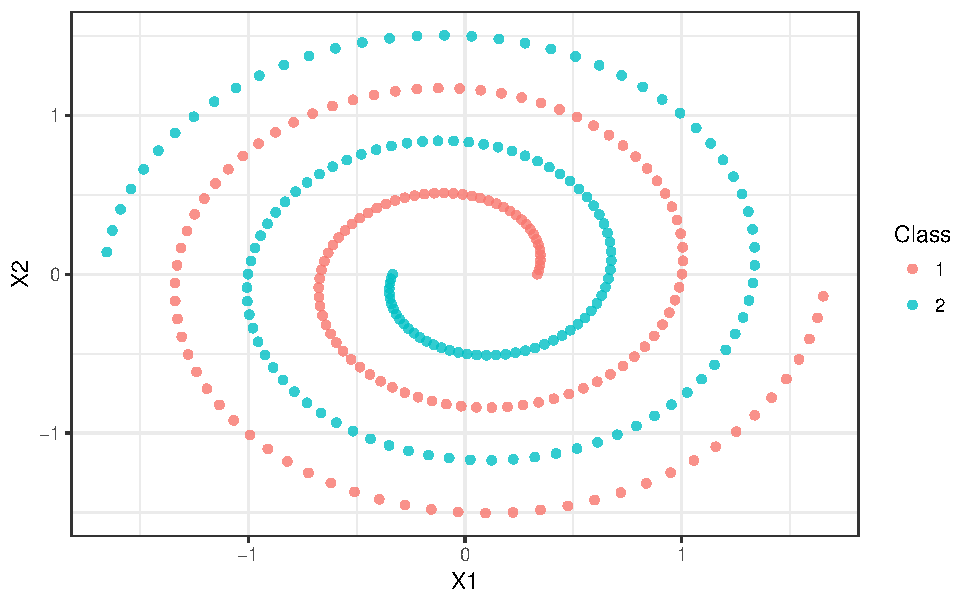
\includegraphics[width=0.7\textwidth]{figure/05-example_data}
  \caption{A scatter plot of simulated spiral data set.}
  \vspace{-0.5em}
  \label{fig:exampleiprobit}
\end{figure}

The three methods pretty much concur on the estimation of the intercept, but not on the RKHS scale parameter.
As a result, the log-density value calculated at the parameter estimates is also different in all three methods.
Notice the high posterior standard deviation for the scale parameter in the HMC method.
The posterior density for $\lambda$ was very positively skewed, and this contributed to the large posterior mean.

\begin{table}[hbt]
\centering
\caption{Table comparing the estimated parameter values, (marginal) log-likelihood values, and also time taken for the three estimation methods.}
\label{tab:compreiprobit}
\begin{tabular}{@{}lrrr@{}}
\toprule
& Laplace approximation 
& Variational EM 
& Hamiltonian MC          \\ \midrule
Intercept ($\alpha$)      & -0.02 (0.03)           & 0.00 (0.06)    & 0.00 (0.58)  \\
Scale ($\lambda$)      & 0.85 (0.01)         & 5.67 (0.23)  & 29.3 (5.21)     \\[0.5em]
Log-density    & -171.8              & -43.2       & -8.5                  \\
Error rate (\%) & 44.7               & 0.00        & 0.00                   \\
Brier score & 0.20               & 0.02        & 0.01                   \\[0.5em]
Iterations     & 20                  & 56          & 2000                    \\
Time taken (s) & >3600                & 5.32         & >1800                     \\ \bottomrule
\end{tabular}
\end{table}


\begin{figure}[p]
  \centering
  \vspace{1em}
  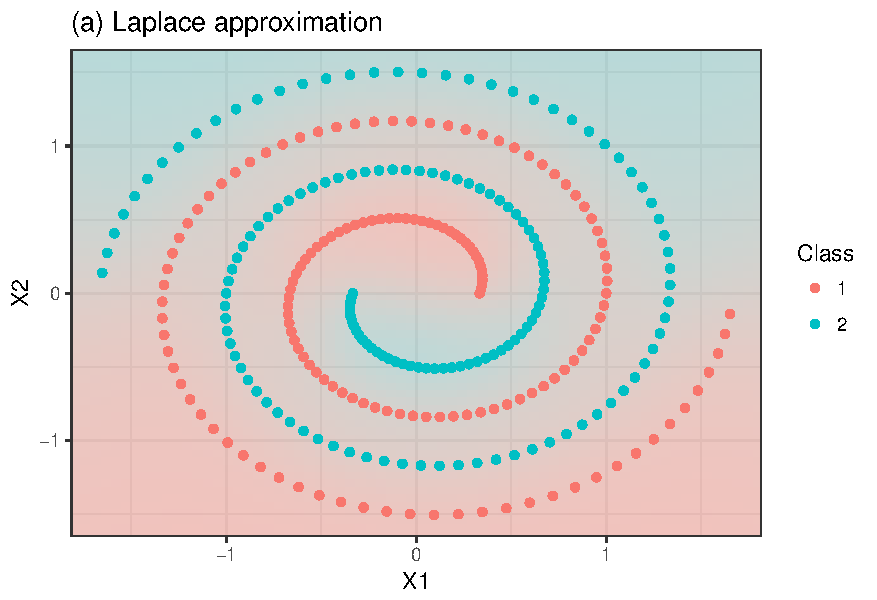
\includegraphics[width=0.49\textwidth]{figure/05-fit_lap}
  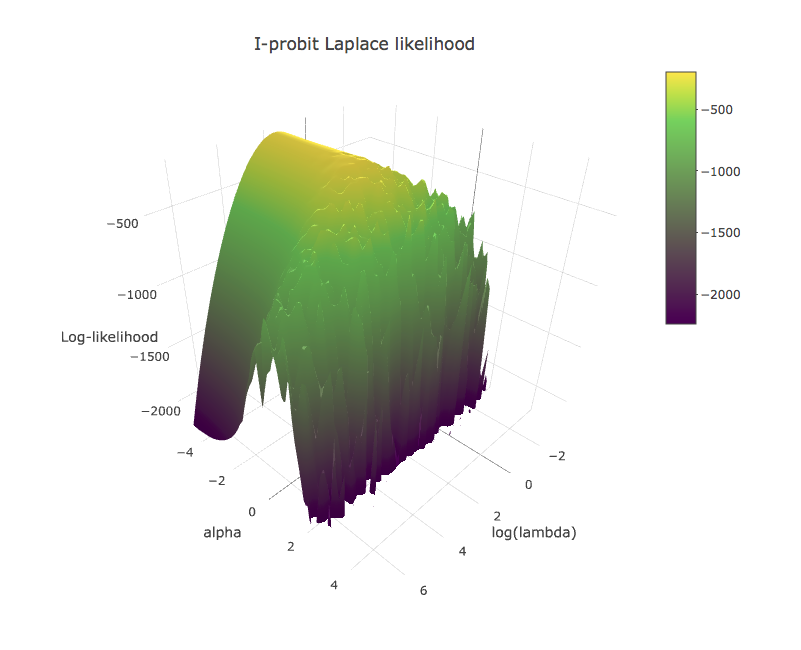
\includegraphics[width=0.49\textwidth]{figure/05-lik_lap}
  \vspace{1em}
  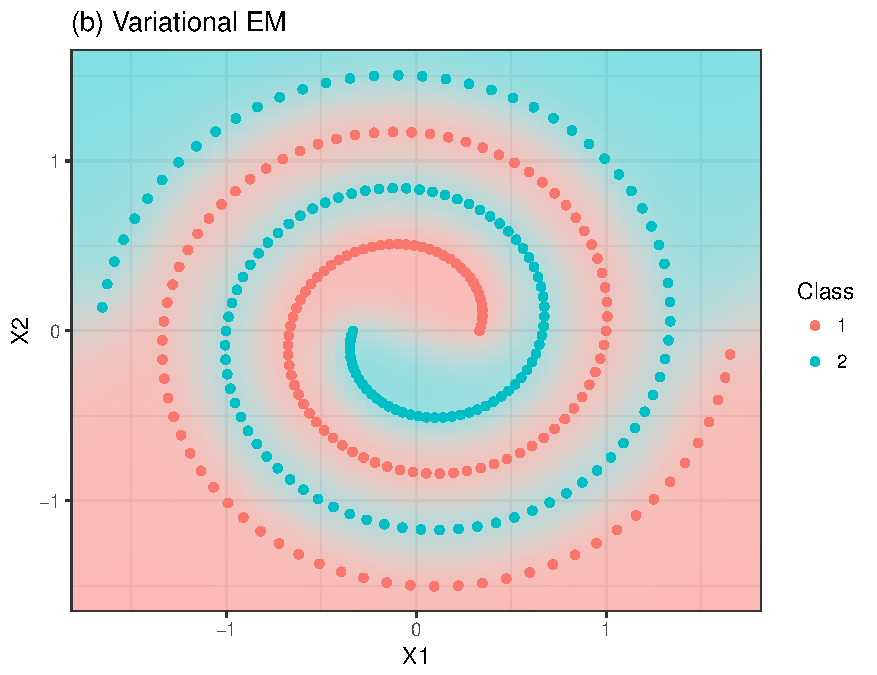
\includegraphics[width=0.49\textwidth]{figure/05-fit_vi}
  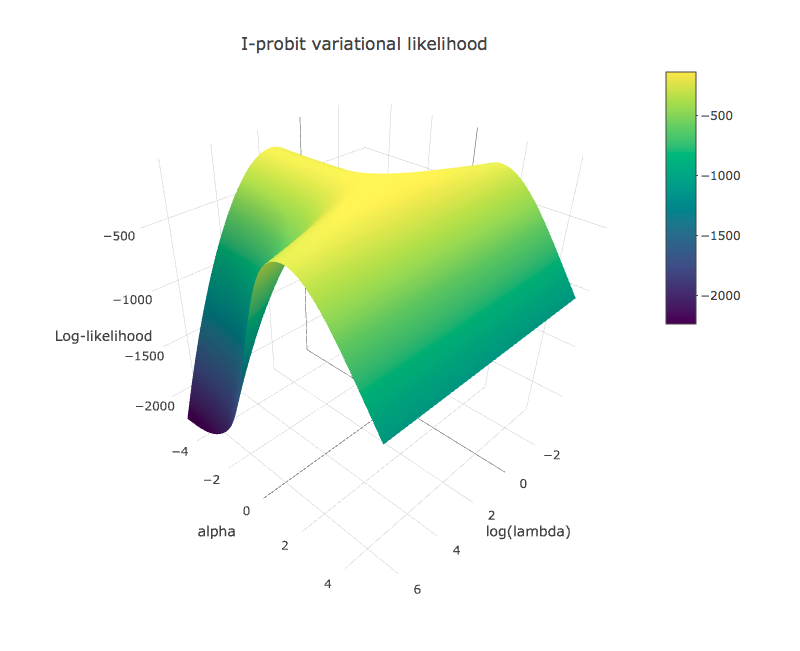
\includegraphics[width=0.49\textwidth]{figure/05-lik_vi}
  \vspace{1em}
  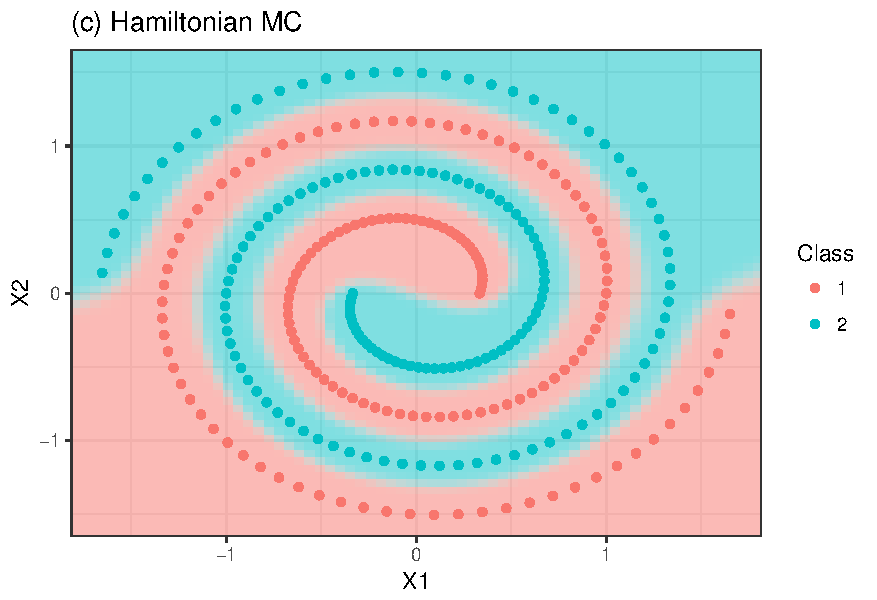
\includegraphics[width=0.49\textwidth]{figure/05-fit_hmc}
  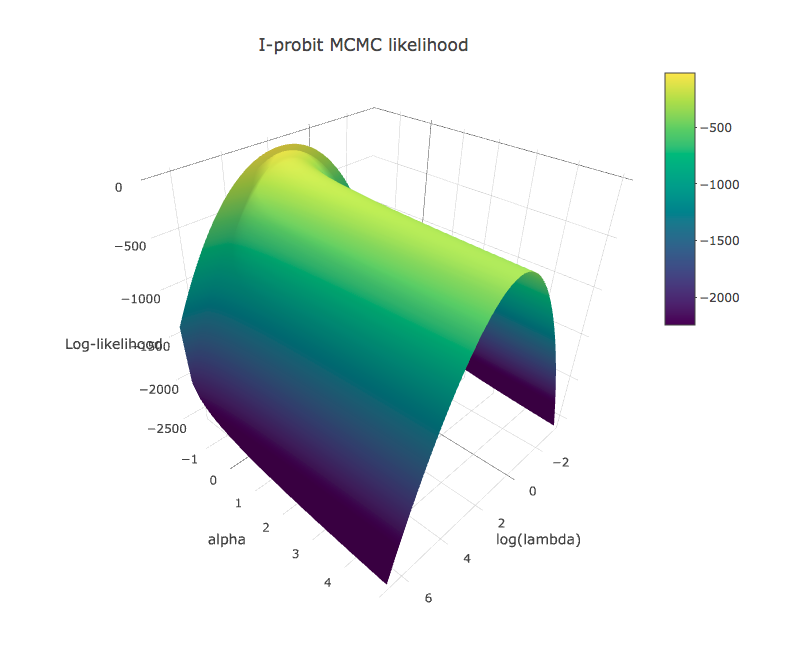
\includegraphics[width=0.49\textwidth]{figure/05-lik_hmc}
  \caption[Predicted probabilities and log-density plots]{Plots showing predicted probabilities (shaded region) for belonging to class `1' or `2' indicated by colour and intensity, and log-likelihood/ELBO surface plots for (a) Laplace's method, (b) variational EM, and (c) Hamiltonian MC. For the Hamiltonian MC plot, parameters are treated as fixed, and the mean log-density of the I-probit model recorded.}
  \label{fig:exampleiprobitfit}
\end{figure}
\index{Brier score}

\index{Laplace's method}
A plot of the log-likelihood (or ELBO) surface for three methods in \cref{fig:exampleiprobitfit} reveals some insight.
The variational likelihood has two ridges, with the maxima occurring around the intersection of these two ridges.
The Laplace likelihood seems to indicate a similar shape---in both the Laplace and variational method, the posterior distribution of $\bw$ is approximated by a Gaussian distribution, with different means and variances.
However, parts of the Laplace likelihood are poorly approximated resulting in a loss of fidelity around the supposed maxima, which might have contributed to the set of values that were estimated.
Laplace's method is known to yield poor approximations to probit model likelihoods \citep{kuss2005assessing}.
On the other hand, the log-likelihood calculated using a Hamiltonian MC sampler (treating parameters as fixed values) yields a slightly different graph: the log-likelihood increases as values of $\alpha$ become larger, resulting in the upwards inflection of the log-likelihood surface (as opposed to a downward inflection seen in the variational and Laplace likelihood).

In terms of predictive abilities, both the variational and Hamiltonian MC methods, even though the posteriors are differently estimated, have good predictive performance as indicated by their error rates and Brier scores\footnote{\index{Brier score}The Brier score is defined as $\frac{1}{n}\sum_{i=1}^n\sum_{j=1}^m (y_{ij} - \hat p_{ij})$ with $y_{ij}=1$ if $y_i = j$ and zero otherwise, and $\hat p_{ij}$ is the fitted probability $\hat\Prob(y_i = j)$. It gives a better sense of ``training/test error'', compared to simple misclassification rates, by accounting for the forecasted probabilities of the events happening. The Brier score is a proper scoring rule, i.e. it is uniquely minimised by the true probabilities.}.
\cref{fig:exampleiprobitfit} shows that HMC is more confident of new data predictions compared to variational inference, as indicated by the intensity of the shaded regions (HMC is shaded stronger than variational EM).
Laplace's method gave poor predictive performance.

Finally, on the computational side, variational inference was by far the fastest method to fit the model.
Sampling using Hamiltonian MC was very slow, because the parameter space is in effect $O(n + 2)$ (parameters are $\{w_1,\dots,w_n,\alpha,\lambda\}$ under the model with likelihood \cref{eq:intractablelikelihood2}, i.e. without the data augmentation scheme).
As for Laplace, each Newton step involves obtaining posterior modes of the $w_i$'s, and this contributed to the slowness of this method.
The reality is that variational inference takes seconds to complete what either the Laplace or full MCMC methods would take minutes or even hours to.
The predictive performance, while not as good as HMC, is certainly an acceptable compromise in favour of speed.
\vspace{-1em}


\section{The variational EM algorithm for I-probit models}\label{sec:iprobitvar}
We present an EM algorithm to estimate the I-probit latent variables $\by^*$ and $\bw$, in which the E-step consists of a mean-field variational approximation of the conditional density $p(\by^*,\bw|\by,\theta) = q(\by^*)q(\bw)$.
As per assumptions $\ref{ass:A4}$, $\ref{ass:A5}$ and $\ref{ass:A6}$, the parameters of the I-probit model consists of $\theta =\{ \balpha = (\alpha_1,\dots,\alpha_m)^\top,\eta \}$.

The algorithm cycles through a variational inference E-step, in which the variational density $q(\by^*,\bw) = \prod_{i=1}^n q(\by^*_{i\bigcdot}) q(\bw)$ is optimised with respect to the Kullbeck-Leibler divergence $\KL\big[ q(\by^*,\bw) \Vert p(\by^*,\bw|\by) \big]$, and an M-step, in which the approximate expected joint density \cref{eq:iprobitQEstep} is maximised with respect to the parameters $\theta$. 
Convergence is assessed by monitoring the ELBO.
Apart from the fact that the variational EM algorithm uses approximate conditional distributions and involves matrices $\by^*$ and $\bw$, it is very similar to the EM described in \cref{chapter4}, and as such, the efficient computational work derived there is applicable.

\subsection{The variational E-step}

Let $\tilde q(\by^*,\bw)$ be the pdf that minimises the Kullbeck-Leibler divergence $\KL\big[ q \Vert p \big]$ subject to the mean-field constraint $q(\by^*,\bw) = q(\by^*)q(\bw)$.
By appealing to \citet[equation 10.9, p. 466]{bishop2006pattern}, the optimal mean-field variational density $\tilde q$ for the latent variables $\by^*$ and $\bw$ satisfy
\begin{align}
  \log \tilde q(\by^*) &= \E_{\bw\sim\tilde q} \big[ \log p(\by,\by^*,\bw) \big] + \const \\
  \log \tilde q(\bw) &= \E_{\by^*\sim\tilde q} \big[ \log p(\by,\by^*,\bw) \big] + \const 
\end{align}
where $p(\by,\by^*,\bw) = p(\by|\by^*) p(\by^*|\bw) p(\bw)$ is as per \cref{eq:iprobitlik}.
We now present the variational densities $\tilde q(\by^*)$ and $\tilde q(\bw)$.
For further details on the derivation of these densities, please refer to the appendix.

\subsubsection{Variational distribution for the latent propensities \texorpdfstring{$\by^*$}{$y^*$}}

The fact that the rows $\by_{i \bigcdot}^* \in \bbR^m$, $i=1,\dots,n$ of $\by^* \in \bbR^{n \times m}$ are independent can be exploited, and this results in a further induced factorisation $q(\by^*) = \prod_{i=1}^n q(\by_i^*)$.
Define the set $\cC_j = \{y_{ij}^* > y_{ik}^* \,|\, \forall k\neq j \}$.
Then $q(\by_{i \bigcdot}^*)$ is the density of a multivariate normal distribution with mean $\tilde \bmu_{i \bigcdot} = \balpha + \tilde\bw^\top  \bh_\eta(x_i)$, where $\tilde \bw = \E_{\bw\sim\tilde q}\bw$, and variance $\bPsi^{-1}$, subject to a truncation of its components to the set $\cC_{y_i}$.
That is, for each $i=1,\dots,n$ and noting the observed categorical response $y_i \in \{1,\dots,m\}$ for the $i$'th observation, the $\by_i^*$'s are distributed according to
\begin{align}\label{eq:ystardist}
  \by_{i \bigcdot}^* \iid
  \begin{cases}
    \N_m(\tilde\bmu_{i \bigcdot},  \bPsi^{-1}) & \text{ if } y_{iy_i}^* > y_{ik}^*, \forall k \neq y_i \\
    0 & \text{ otherwise}. \\
  \end{cases}
\end{align}
We denote this by $\by_{i \bigcdot}^* \iid \tN(\tilde\bmu_{i \bigcdot}, \bPsi^{-1},\cC_{y_i})$, and the important properties of this distribution are explored in the appendix.

The required expectation $\tilde\by^* := \E_{\by^*\sim\tilde q}\by^*_{i\bigcdot} = \E_{\by^*\sim\tilde q} (y_{i1}^*,\dots, y_{im}^*)^\top$ in the M-step can be tricky to obtain.
One strategy that can be considered is Monte Carlo integration: using samples from $\N_m(\tilde\bmu_{i \bigcdot},  \bPsi^{-1})$, disregard those that do not satisfy the condition $y_{iy_i}^* > y_{ik}^*, \forall k \neq j$, and then take the sample average.
This works reasonably well so long as the truncation region does not fall into the extreme tails of the multivariate normal.
Alternatively, a fast, Gibbs-based approach \citep{robert1995simulation} for sampling from a truncated multivariate normal can be implemented, and this is detailed in the appendix.

If the independent I-probit model is under consideration, whereby the covariance matrix has the independent structure $\bPsi = \diag(\sigma_1^{-2},\dots,\sigma_m^{-2})$, then the first moment  can be considered component-wise. 
Each component of this expectation is given by
\begin{align}\label{eq:ystarupdate}
  \tilde y_{ik}^* =
  \begin{cases}
    \tilde\mu_{ik} - \sigma_k C_i^{-1} \displaystyle{  \int \phi_{ik}(z) \prod_{l \neq k,y_i} \Phi_{il}(z) \phi(z) \dint z }
    &\text{ if } k \neq y_i \\[1.5em]
    \tilde\mu_{iy_i} - \sigma_{y_i} \sum_{k \neq y_i} \big(\tilde y_{ik}^* -  \tilde\mu_{ik} \big) 
    &\text{ if } k = y_i \\
  \end{cases}
\end{align}
with 
\begin{align*}
  \phi_{ik}(Z) &= \phi \left(\frac{\sigma_{y_i}}{\sigma_k} Z + \frac{\tilde\mu_{iy_i} - \tilde\mu_{ik}}{\sigma_k} \right) \\
  \Phi_{ik}(Z) &= \Phi \left(\frac{\sigma_{y_i}}{\sigma_k} Z + \frac{\tilde\mu_{iy_i} - \tilde\mu_{ik}}{\sigma_k} \right) \\
  C_i &= \int \prod_{l \neq j} \Phi_{il}(z) \phi(z) \dint z
\end{align*}
and $Z \sim \N(0,1)$ with pdf and cdf $\phi(\cdot)$ and $\Phi(\cdot)$ respectively. 
The integrals that appear above are functions of a unidimensional Gaussian pdf, and these can be computed rather efficiently using quadrature methods.

\subsubsection{Variational distribution for the I-prior random effects \texorpdfstring{$\bw$}{$w$}}

Given that both $\vecc \by^* | \vecc \bw$ and $\vecc\bw$ are normally distributed as per the model \cref{eq:iprobitmod}, we find that the full conditional distribution $p(\bw|\by^*,\by) \propto p(\by^*,\by,\bw) \propto p(\by^*|\bw)p(\bw)$ is also normal. 
The variational density $q$ for $\vecc \bw \in \bbR^{nm}$ is found to be Gaussian with mean and precision given by
\begin{gather}\label{eq:varipostw}
   \vecc \tilde\bw = \tilde\bV_w 
    (\bPsi \otimes \bH_\eta) \vecc (\tilde\by^* - \bone_n\balpha^\top)
  \hspace{0.5cm}\text{and}\hspace{0.5cm} 
  \tilde \bV_w^{-1} = \bPsi \otimes \bH_\eta^2 + \bPsi^{-1} \otimes \bI_n = \bV_{y^*}.
\end{gather}
As a computational remark, computing the inverse $\tilde\bV_w^{-1}$ presents a challenge, as this takes $O(n^3m^3)$ time if computed naïvely. 
By exploiting the Kronecker product structure in $\tilde\bV_w$, we are able to efficiently compute the required inverse in roughly $O(n^3m)$ time---see the \hltodo{Section X} for details.
Storage requirement is $O(n^2m^2)$, as a result of the covariance matrix in \cref{eq:varipostw}.

If the independent I-probit model is assumed, i.e. $\bPsi = \diag(\psi_1,\dots,\psi_m)$, then the posterior covariance matrix $\tilde\bV_w$ has a simpler structure which implies column independence in the matrix $\bw$.
By writing $\bw_{\bigcdot j} = (w_{1j},\dots,w_{nj})^\top \in \bbR^n$, $j=1,\dots,m$, to denote the column vectors of $\bw$, and with a slight abuse of notation, we have that
\begin{align*}
  \N_{nm}(\vecc \bw|\vecc\wtilde, \tilde\bV_w) 
  = \prod_{j=1}^m \N_{n}(\bw_{\bigcdot j}|\tilde\bw_{\bigcdot j}, \tilde\bV_{w_j}),
\end{align*}
where 
\[
  \tilde \bw_{\bigcdot j} = \psi_j\tilde \bV_{w_j}\bH_\eta (\tilde\by^*_j - \alpha_j\bone_n) \ \text{ and } \ \tilde \bV_{w_j} = \big(\psi_j\bH_{\eta}^2 + \psi_j^{-1}\bI_n \big)^{-1}.
\]
We note the similarity between \cref{eq:varipostw} above and the posterior distribution for the I-prior random effects in a normal model \cref{eq:posteriorw} seen in the previous chapter, with the difference being \cref{eq:varipostw} uses the continuous latent propensities $\by^*$ instead of the the observations $\by$.
The consequence of this is that the posterior regression functions are class independent, the exact intended effect by specifying a diagonal precision matrix $\bPsi$.
Storage requirement is $O(n^2m)$, since we need $\bV_{w_1},\dots,\bV_{w_m}$.

\begin{remark}
  The variational distribution $q(\bw)$ which approximates $p(\bw|\by)$ is in fact exactly $p(\bw|\by^*)$, the conditional density of the I-prior random effects given the latent propensities.
  By the law of total expectations, 
  \begin{gather*}
    \E[r(\bw)|\by] = \E_{\by^*}\big[ \E[r(\bw)|\by^*] \,|\, \by \big],
  \end{gather*}
  where $r(\cdot)$ is some function of $\bw$, and expectations are taken under the posterior distribution of $\by^*$.
  Hypothetically, if the true pdf $p(\by^*|\by)$ were tractable,  then the E-step can be computed using the true conditional distribution.
  Since it is not tractable, we resort to an approximation, and in the case of a variational approximation, \cref{eq:varipostw} is obtained.
\end{remark}



\subsection{The M-step}
\label{sec:varupdeta}

From \cref{eq:iprobitQEstep}, the function to be maximised in the M-step is
\begin{align*}
  Q(\theta) 
  &=\const -\half\tr\Big( \bPsi\E[\bw^\top\bH_\eta^2\bw]  + \bPsi^{-1} \E[\bw^\top\bw] \Big)   \\
  &\phantom{==} - \half \tr \Big( 
  \bPsi \Big( 
  \E[\by^{*\top}\by^*]
  + n \balpha\balpha^\top 
  - 2\tilde\by^{*\top}\bone_n \balpha^\top 
  - 2\tilde\bw^\top\bH_\eta (\tilde\by^* - \bone_n\balpha^\top) 
  \Big) \Big) \tag{\ref{eq:iprobitQEstep}}
  ,
\end{align*}
where expectations are taken with respect to the variational distributions of $\by^*$ and $\bw$. 
Note that since $\bPsi$ is treated as fixed, the term $\E[\by^{*\top}\by^*]$ is absorbed into the constant.
On closer inspection, the trace involving the second moments of $\bw$ is found to be
\begin{align*}
  \tr \Big( \bPsi\E[\bw^\top\bH_\eta^2\bw]  + \bPsi^{-1} \E[\bw^\top\bw] \Big)
  &= \sum_{i,j=1}^m \left\{ \psi_{ij} \tr(\bH_\eta^2\tilde\bW_{ij}) + \psi_{ij}^- \tr(\tilde\bW_{ij}) \right\}
\end{align*}
by the results of \hltodo{equation} derived in the appendix.
In the above, we had defined $\psi_{ij}^-$ to be the $(i,j)$'th element of $\bPsi^{-1}$, and
\[
  \tilde\bW_{ij} 
  = \E[\bw_{\bigcdot i}\bw_{\bigcdot j}^\top]
  =  \bV_{w}[i,j] + \tilde\bw_{\bigcdot i} \tilde\bw_{\bigcdot j}^\top,
\]
where $\bV_{w}[i,j] \in \bbR^{n\times n}$ refers to the $(i,j)$'th submatrix block of $\bV_w$, and the $n$-vector $\tilde \bw_{\bigcdot j} = \big(\E [w_{ij}] \big)_{i=1}^n$ is the expected value of the random effects for class $j$.
Specifically, when the error precision is of the form $\bPsi = \diag(\psi_1,\dots,\psi_m)$, this trace reduces to
\begin{align*}
  \tr \Big( \bPsi\E[\bw^\top\bH_\eta^2\bw]  + \bPsi^{-1} \E[\bw^\top\bw] \Big)
  &= \sum_{j=1}^m \left\{ \psi_j \tr(\bH_\eta^2\tilde\bW_{jj}) + \psi_j^{-1} \tr(\tilde\bW_{jj}) \right\} \\
  &= \sum_{j=1}^m \tr\big( 
  (\greyoverbrace{\psi_j\bH_\eta^2 + \psi_j^{-1}\bI_n}{\bSigma_{\theta,j}}) 
  \tilde\bW_{jj} \big)
\end{align*}

The bulk of the computational effort required to evaluate $Q(\theta)$ stems from the trace involving the second moments of $\bw$, and the fact that $\bH_\eta^2$ needs to be reevaluated each time $\theta = \{\balpha,\eta\}$ changes.
As discussed previously, each E-step takes $O(n^3m)$ time to compute the required first and second (approximate) posterior moments of $\bw$.
Once this is done, we can use the `front-loading of the kernel matrices' trick described in \cref{sec:efficientEM1}, which effectively renders the evaluation of $Q$ to be linear in $\theta$ (after an initial $O(n^2)$ procedure at the beginning).

As in the normal linear model, we employ a sequential update of the parameters (à la expectation conditional maximisation algorithm) by solving the first order conditions
\begin{align}
  \frac{\partial}{\partial\eta}Q(\eta|\balpha)
  &= -\half \sum_{i,j=1}^m \psi_{ij} \tr \left( \frac{\partial \bH_\eta^2}{\partial\eta} \tilde\bW_{ij} \right) 
  + \tr\left( \bPsi \tilde\bw^\top  \frac{\partial \bH_\eta}{\partial\eta} (\tilde\by^* - \bone_n\balpha^\top)  \right) \label{eq:vemeta} \\
  \frac{\partial}{\partial\balpha}Q(\balpha|\eta)
  &= 2n\bPsi\balpha - 2 \sum_{i=1}^n \bPsi \big(\by_{i\bigcdot}^* - \tilde\bw^\top\bh_\eta(x_i) \big) \label{eq:vemalpha}
\end{align}
equated to zero, where $\bh_\eta(x_i) \in \bbR^n$ is the $i$'th row of the kernel matrix $\bH_\eta$.
We now present the update equations for the parameters.

\subsubsection{Update for kernel parameters $\eta$}

When only ANOVA RKHS scale parameters are involved, then the conditional solution of $\eta$ to \cref{eq:vemeta} can be found in closed-form, much like in the exponential family EM algorithm described in \cref{sec:expfamEM}.
Under the same setting as in that subsection, assume that only $\eta = \{\lambda_1,\dots,\lambda_p\}$ need be estimated, and for each $k=1,\dots,p$, we can decompose the kernel matrix as $\bH_\eta = \lambda_k \bR_k + \bS_k$ and its square as $\bH_\eta^2 = \lambda_k^2 \bR_k^2 + \lambda_k \bU_k + \bS_k^2$.
As a follow-on from \cref{eq:vemeta}, the conditional solution for $\lambda_k$ given the rest of the parameters is obtained by solving
\begin{align*}
  \frac{\partial}{\partial\lambda_k}Q(\lambda_k|\balpha,\blambda_{-k})
  &= -\half \sum_{i,j=1}^m \psi_{ij} \tr \left( (2\lambda_k\bR_k^2 + \bU_k) \tilde\bW_{ij} \right) 
  + \tr\left( \bPsi \tilde\bw^\top \bR_k (\tilde\by^* - \bone_n\balpha^\top)  \right) \\
  &= - \lambda_k \sum_{i,j=1}^m \psi_{ij} \tr(\bR_k^2\tilde\bW_{ij})
  - \half \sum_{i,j=1}^m \psi_{ij} \tr(\bU_k\tilde\bW_{ij}) \\
  &\phantom{==} + \tr\left( \bPsi \tilde\bw^\top \bR_k (\tilde\by^* - \bone_n\balpha^\top)  \right) \\
  &=0.
\end{align*}
This yields the solution
\[
  \hat\lambda_k 
  = \frac{
  \tr\left( \bPsi \tilde\bw^\top \bR_k (\tilde\by^* - \bone_n\balpha^\top) \right)
  - \half \sum_{i,j=1}^m \psi_{ij} \tr(\bU_k\tilde\bW_{ij})
  }{
  \sum_{i,j=1}^m \psi_{ij} \tr(\bR_k^2\tilde\bW_{ij})
  }
\]
In the case of the independent I-probit model, where $\bPsi = \diag(\psi_1,\dots,\psi_m)$, $\hat\lambda_k$ has the form
\[
  \hat\lambda_k
  = \frac{
  \sum_{j=1}^m \psi_j \left( \tilde\bw^\top_{\bigcdot j} \bR_k (\tilde\by^*_{\bigcdot j} - \alpha_j\bone_n) - \half \tr(\bU_k\tilde\bW_{jj})\right)
  }{
  \sum_{j=1}^m \psi_j \tr(\bR_k^2\tilde\bW_{jj})
  }.
\]

\begin{remark}
  There is no closed-form solution for $\eta$ when the polynomial kernel is used, or when there are kernel parameters to optimise (e.g. Hurst coefficient or SE kernel lengthscale).
  In these situations, solutions for $\eta$ are obtained using numerical methods (i.e. employ quasi-Newton methods such as L-BFGS algorithm for optimising $Q(\eta|\balpha)$).
\end{remark}

\subsubsection{Update for intercepts \texorpdfstring{$\balpha$}{$\alpha$}}

It is easy to see that the unique solution to \cref{eq:vemalpha} is
\begin{align*}
  \hat\balpha
  &= \frac{1}{n} \bPsi^{-1} \left( \sum_{i=1}^n \bPsi \big(\by_{i\bigcdot}^* - \tilde\bw^\top\bh_\eta(x_i) \big) \right) 
  =\frac{1}{n} \sum_{i=1}^n \big(\by_{i\bigcdot}^* - \tilde\bw^\top\bh_\eta(x_i) \big) \in \bbR^m.
\end{align*}
Being free of $\bPsi$, the solution is the same whether the full or independent I-probit model is assumed.
Furthermore, we must have that $\sum_{j=1}^m \alpha_j = 0$ for identifiability, so as an additional step to satisfy this condition, the solution $\balpha$ is centred.

\subsection{Summary}

A summary of the variational EM algorithm is presented.
Notice that the evaluation of each component of the posterior depends on knowing the posterior distribution of the other, i.e. $q(\by^*)$ depends on $q(\bw)$ and vice-versa.
Similarly, each parameter update is obtained conditional upon the value of the rest of the parameters.
These circular dependencies are dealt with by way of an iterative updating scheme: with arbitrary starting values for the distributions $q^{(0)}(\by^*)$ and $q^{(0)}(\bw)$, and for the parameters $\theta^{(0)}$, each are updated in turn according to the above derivations.

The updating sequence is repeated until no significant increase in the convergence criterion, the ELBO, is observed.
The ELBO for the I-probit model is given by the quantity
\begin{align}
  \cL_q(\theta) = \half[nm] + \sum_{i=1}^n \log C_i(\theta) + \half\log \abs{\tilde\bV_w} - \half[n]\log\abs{\bPsi} - \half\sum_{i,j=1}^m \psi_{ij}^- \tr(\tilde\bW_{ij}),
\end{align}
where $C_i(\theta)$ is the normalising constant of the distribution $\tN_m(\balpha + \bw^\top\bh_\eta(x_i),\bPsi^{-1},\cC_{y_i})$, with $\cC_{y_i} = \{y_{iy_i}^* > y_{ik}^* | \forall k \neq y_i \}$.
That is,
\[
  C_i(\theta) = \idotsint\displaylimits_{\{y_{iy_i}^* > y_{ik}^* | \forall k \neq y_i \}} \phi(y_{i1}^*, \dots, y_{im}^*|\balpha + \bw^\top\bh_\eta(x_i), \bPsi^{-1}) \dint y_{i1}^* \cdots \dint y_{im}^*.
\]
Similar to the EM algorithm, each iteration of the algorithm increases the ELBO to a stationary point \citep{blei2017variational}.
Unlike the EM algorithm though, the variational EM algorithm does \emph{not} guarantee an increase in the marginal log-likelihood at each step, nor does it guarantee convergence to the global maxima of the log-likelihood.

Further, the ELBO expression to be maximised is often not convex, which means the CAVI algorithm may terminate at local modes, for which they may be many.
Note that the variational distribution with the higher ELBO value is the distribution that is closer, in terms of the KL divergence, to the true posterior distribution.
In our experience, multiple random starts alleviates this issue for the I-probit model.

\algrenewcommand{\algorithmiccomment}[1]{{\color{gray} \hfill $\triangleright$ #1}}
\begin{algorithm}[p]
\caption{Variational EM for the I-probit model (fixed $\bPsi$)}\label{alg:varemiprobit}
\begin{algorithmic}[1]
  \Procedure{Initialisation}{}
    \State Initialise $\theta^{(0)} \gets \{\balpha^{(0)},\eta^{(0)}\}$
    \State $\tilde q^{(0)}(\bw) \gets \MN(\bzero,\bI_n,\bPsi)$
    \State $\tilde q^{(0)}(\by^*_{i\bigcdot}) \gets \tN_m(\tilde\balpha^{(0)},\bPsi^{-1},\cC_{y_i})$
    \State $t \gets 0$
  \EndProcedure 
  \Statex
  \While{not converged}{}
    \Procedure{Variational E-step}{}
      \For{$i=1,\dots,n$} \Comment{Update $\by^*$}
        \State $\tilde q^{(t+1)}(\by^*_{i \bigcdot}) \gets \tN_m\big(\tilde\balpha^{(t)} + \tilde\bw^{(t)\top} \bh_{\eta^{(t)}}(x_i), \bPsi, \cC_{y_i}\big)$ 
        \State $\tilde \by^{*(t+1)}_{i \bigcdot} \gets \E_{q^{(t+1)}}[\by^*_{i \bigcdot}]$
      \EndFor
      \Statex
      \State $\tilde\bV_w^{(t+1)} \gets \big((\bPsi \otimes \bH_{\eta^{(t)}}^2) + (\bPsi^{-1} \otimes \bI_n)\big)^{-1}$ \Comment{Update $\bw$}
      \State $\vecc\tilde\bw^{(t+1)}  \gets \tilde\bV_w^{(t+1)} 
      (\bPsi \otimes \bH_{\eta^{(t)}}) \vecc (\tilde\by^{*(t+1)} - \bone_n\balpha^{(t)\top})$
      \State $\tilde q^{(t+1)}(\bw) \gets \N_{nm}\big( \vecc \tilde\bw^{(t+1)}, \tilde\bV_w^{(t+1)} \big)$ 
    \EndProcedure
    \Statex
    \Procedure{M-step}{}
      \If{ANOVA kernel (closed-form updates)} \Comment{Update $\eta$}
        \For{$k=1,\dots,p$} 
          \State $T_{1k} \gets \sum_{i,j=1}^m \psi_{ij} \tr(\bR_k^2\tilde\bW_{ij})$ 
          \State $T_{2k} \gets \tr\left( \bPsi \tilde\bw^\top \bR_k (\tilde\by^* - \bone_n\balpha^\top) \right) - \half \sum_{i,j=1}^m \psi_{ij} \tr(\bU_k\tilde\bW_{ij})$ 
          \State $\lambda_k^{(t+1)} \gets T_{2k}/T_{1k}$           
        \EndFor
      \Else
        \State $\eta^{(t+1)} \gets \argmax_\eta Q(\eta|\balpha^{(t)})$ by L-BFGS algorithm
      \EndIf
      \Statex
      \State $\ba \gets \frac{1}{n} \sum_{i=1}^n \big( \tilde\by^{*(t+1)}_{i \bigcdot} - \tilde\bw^{(t+1)\top} \tilde\bh_{\eta^{(t+1)}}(x_i) \big)$ \Comment{Update $\balpha$}
      \State $\balpha^{(t+1)} \gets \ba - \frac{1}{m}\sum_{j=1}^m a_j$
    \EndProcedure
    \Statex
    \State Calculate ELBO $\cL^{(t+1)}$
    \State $t \gets t + 1$
  \EndWhile
\end{algorithmic}
\end{algorithm}


\section{Post-estimation}\label{sec:iprobitpostest}
\index{I-probit!posterior distribution}
Post-estimation procedures such as obtaining predictions for a new data point, the credibility interval for such predictions, and model comparison, are of interest.
These are performed in an empirical Bayes manner using the variational posterior density of the regression function obtained from the output of the variational EM algorithm.

We first describe prediction of a new data point $x_{\text{new}}$.
Step one is to determine the distribution of the posterior regression functions in each class, $\bff(x_{\text{new}}) = \bw^\top\bh_\eta(x_{\text{new}})$, where $\bh_\eta(x_{\text{new}})$ is the vector of length $n$ containing entries $h_\eta(x_i,x_\new)$, given values for the parameters $\theta$ of the I-probit model.
To this end, we use the ELBO estimates for $\theta$, i.e. $\hat\theta = \argmax_\theta \cL_q(\theta)$, as obtained from the variational EM algorithm.
As we know, the variational distribution of $\vecc\bw$ is normally distributed with mean and variance according to \cref{eq:varipostw}.
By writing $\vecc \tilde\bw = (\tilde \bw_{\bigcdot 1}, \dots, \tilde \bw_{\bigcdot m})^\top$ to separate out the I-prior random effects per class, we have that $\bw_{\bigcdot j}|\hat\theta \sim \N_n(\tilde \bw_{\bigcdot j}, \tilde\bV_w[j,j])$, and $\Cov(\bw_{\bigcdot j},\bw_{\bigcdot k}) = \tilde\bV_w[j,k]$, where the `$[\cdot,\cdot]$' indexes the $n\times n$ sub-block of the block matrix $\bV_w$.
Thus, for each class $j=1,\dots,m$ and any $x \in \cX$,
\[
  f_j(x)|\by,\hat\theta \sim \N\Big(\,
  \bh_{\hat\eta}(x)^\top \tilde\bw_{\bigcdot j} \, , \,
  \bh_{\hat\eta}(x)^\top\tilde\bV_w[j,j] \, \bh_{\hat\eta}(x)
  \Big),
\]
and the covariance between the regression functions in two different classes is
\[
  \Cov\big(f_j(x),f_k(x)|\by,\hat\theta \big) = 
  \bh_{\hat\eta}(x)^\top \tilde\bV_w[j,k] \, \tilde\bh_{\hat\eta}(x).
\]
\index{I-probit!posterior predictive distribution}Then, in step two, using the results obtained in the previous chapter in \cref{sec:ipriorpostest} \colp{\mypageref{sec:ipriorpostest}}, we have that the latent propensities $y_{\new,j}^*$ for each class are normally distributed with mean, variance, and covariances
\begin{alignat*}{3}
  \E(y_{\new,j}^*|\by,\hat\theta) 
  &= \hat\alpha_j + \E \big( f_j(x_\new) |\by,\hat\theta \big)
  &&=: \hat\mu_j(x_\text{new}) \\
  \Var(y_{\new,j}^*|\by,\hat\theta) 
  &= \Var\big(f(x_\new)|\by,\hat\theta \big) + \bPsi^{-1}_{jj}
  &&=: \hat\sigma_j^2(x_\text{new}) \\
  \Cov(y_{\new,j}^*,y_{\new,k}^*|\by,\hat\theta)
  &= \Cov\big(f_j(x),f_k(x)|\by,\hat\theta \big) + \bPsi^{-1}_{jk}
  &&=: \hat\sigma_{jk}(x_\text{new}).
\end{alignat*}

From here, step three would be to extract class information of data point $x_\text{new}$, which are contained in the normal distribution $\N_{m}\big(\hat\bmu_\new, \hat\bV_\new \big)$, where
\begin{equation*}
  \hat\bmu_\new = \big(\mu_1(x_\text{new}),\dots, \mu_m(x_\text{new}) \big)^\top 
  \hspace{0.5cm}\text{and}\hspace{0.5cm}
  \hat\bV_{\new,jk} = 
  \begin{cases}
    \hat\sigma_j^2(x_\text{new}) & \text{if } j = k \\
    \hat\sigma_{jk}(x_\text{new}) & \text{if } j \neq k. \\
  \end{cases}
\end{equation*}
The predicted class is inferred from the latent variables using
\[
  \hat y_{\text{new}} = \argmax_k \hat\mu_k(x_\new), 
\]
while the probabilities for each class are obtained by way of integration of a multivariate normal density, as per \cref{eq:pij}:
\begin{align}
  \hat p_{\text{new},j} 
  &=  \idotsint\displaylimits_{\{y^*_j > y^*_k | \forall k \neq j \}} \phi(y_{1}^*, \dots, y_{m}^*|\hat\bmu_\new, \hat\bV_{\new}) \dint y_{1}^* \cdots \dint y_{m}^*.
\end{align}
For the independent I-probit model, class probabilities are obtained in a more compact manner via
\[
  \hat p_{\text{new},j} 
  = \E_Z \Bigg[ \mathop{\prod_{k=1}^m}_{k\neq j} 
  \Phi \left(\frac{\hat\sigma_j(x_\text{new})}{\hat\sigma_k(x_\text{new})} Z + \frac{\hat\mu_j(x_\new) - \hat\mu_k(x_\new)}{\hat\sigma_k^2(x_\text{new})} \right) \Bigg],
\]
as per \cref{eq:pij2}, since the $m$ components of $\bff(x_\new)$, and hence the $\by^*_{\new,j}$'s, are independent of each other ($\bPsi$ and $\hat\bV_\new$ are diagonal).
Prediction of a single new data point takes $O(n^2m)$ time, because there are essentially $m$ I-prior posterior regression functions, and each take $O(n^2)$ to evaluate.
This is assuming negligible time to compute the class probabilities.

\index{credibility interval}
We are able to take advantage of the Bayesian machinery to obtain credibility intervals for probability estimates or any transformation of these probabilities (e.g. log odds or odds ratios).
The procedure is as follows.
First, obtain samples $\bw^{(1)},\dots,\bw^{(T)}$ by drawing from its variational posterior distribution $\vecc\bw^{(t)}|\hat\theta \sim \N_{nm}(\vecc \tilde\bw,\bV_w)$.
Then, obtain samples of class probabilities $\{p_{xj}^{(1)},\dots, p_{xj}^{(T)} \}_{j=1}^m$, for a given data point $x\in\cX$ by evaluating
\[
  p_{xj}^{(t)} = \idotsint\displaylimits_{\{y^*_j > y^*_k | \forall k \neq j \}} \phi\big(y_{1}^*, \dots, y_{m}^*|\hat\bmu^{(t)}(x), \hat\bV(x)\big) \dint y_{1}^* \cdots \dint y_{m}^*,
\]
where $\hat\bmu^{(t)}(x) = \hat\balpha + \bw^{(t)\top}\bh_{\hat\eta}(x)$, and $\hat\bV(x)_{jk}$ equals $\hat\sigma^2_j(x)$ if $j = k$, and $\hat\sigma_{jk}(x)$ otherwise.
To obtain a statistic of interest, say, a 95\% credibility interval of a function $r(p_{xj})$ of the probabilities, simply take the empirical lower 2.5th and upper 97.5th percentile of the transformed sample $\big\{ r(p_{xj}^{(1)}),\dots, r(p_{xj}^{(T)}) \big\}$.
%In this manner, all aspects of uncertainty, from the parameters to the latent variables of the generative model, are accounted for.

\begin{remark}
  \index{bootstrap}
  \index{variational EM algorithm!standard error}
  \index{standard error}
  Unfortunately, with the variational EM algorithm, standard errors for the parameters $\theta$ are not so easy to obtain.  
  We could not ascertain as to the availability of an unbiased estimate of the asymptotic covariance matrix for $\theta$ under a variational framework.
  One strategy for obtaining standard errors is bootstrap \citep{chen2017use}:
  \begin{enumerate}
    \item Obtain $\hat\theta = \argmax_\theta \cL_q(\theta)$ using $\cS = \{(y_1,x_1),\dots, (y_n,x_n)\}$.
    \item For $t=1,\dots,T$, do
    \begin{enumerate}
      \item Obtain $\cS^{(t)} = \{ (y_1^{(t)},x_1^{(t)}),\dots, (y_n^{(t)},x_n^{(t)})\}$ by sampling $n$ points with replacement from $\cS$.
      \item Compute $\hat\theta^{(t)} = \argmax_\theta \cL_q(\theta)$ using the data $\cS^{(t)}$.
    \end{enumerate}
    \item For the $l$'th component of $\theta$, compute its variance estimator using
    \[
      \widehat\Var(\hat\theta_l) = \frac{1}{T} \sum_{t=1}^T (\hat\theta_l^{(t)} - \bar\theta_l)^2
      \hspace{0.5cm}\text{where}\hspace{0.5cm}
      \bar\theta_l = \frac{1}{T} \sum_{t=1}^T \hat\theta_l^{(t)}.
    \]
%    where
%    \[
%      \bar\theta_l = \frac{1}{T} \sum_{t=1}^T \hat\theta_l^{(t)}.
%    \]
  \end{enumerate}
  The obvious potential downside to this bootstrapp scheme is computational time.
\end{remark}

\index{Bayes factor!empirical}
\index{empirical Bayes factor|see{Bayes factor}}
Finally, a discussion on model comparison, which, in the variational inference literature, is achieved by comparing ELBO values of competing models \citep{beal2003}.
The rationale is that the ELBO serves as a conservative estimate for the log marginal likelihood, which would allow model selection via (empirical) Bayes factors.
This stems from the fact that 
\begin{align*}
  \log p(\by|\theta) 
  &= \cL_q(\theta) + \KL(q \Vert p ) 
  > \cL_q(\theta),
\end{align*}
since the Kullback-Leibler divergence from the true posterior density $p(\by^*,\bw|\by)$ to the variational density $q(\by^*,\bw)$ is strictly positive (it is zero if and only if the two densities are equivalent), and is minimised under a variational inference scheme.
\citet{kass1995bayes} suggest \cref{tab:BF} as a way of interpreting  observed Bayes factor values $\BF(M_1,M_0)$ for comparing model $M_1$ against model $M_0$, where $\BF(M_1,M_0)$ is approximated by
\[
  \BF(M_1,M_0) \approx \frac{\cL_q(\theta|M_1)}{\cL_q(\theta|M_0)},
\]
and $\cL_q(\theta|M_k)$, $k=0,1$, is the ELBO for model $M_k$.
It should be noted that while this works in practice, there is no theoretical basis for model comparison using the ELBO \citep{blei2017variational}.

\index{Bayes factor}
\vspace{0.3em}
\begin{table}[htbp]\label{tab:BF}
  \centering
  \caption[Guidelines for interpreting Bayes factors]{Guidelines for interpreting Bayes factors \citep{kass1995bayes}.}
  \label{tab:bf}
  \begin{tabular}{lll}
    \toprule
    $2\log \BF(M_1,M_0)$ &$\BF(M_1,M_0)$ & Evidence against $M_0$ \\
    \midrule
    0--2  &1--3    &Not worth more than a bare mention \\ 
    2--6  &3--20   &Positive \\ 
    6--10 &20--150 &Strong \\ 
    >10   &>150    &Very strong \\ 
  \end{tabular}
\end{table}

\begin{remark}
  In the previous chapter on normal I-prior models, the I-prior could be integrated out of the model completely, resulting in a normal  log-likelihood for the parameters.
  Model comparison can be validly done using likelihood ratio tests and asymptotic chi-square distributions.
  Here however, we only have a lower bound to the log-likelihood, and most likely the asymptotic results of likelihood ratio tests do not hold.
  Then, the concept of approximate (empirical) Bayes factors seem most intuitive, even if not rooted in theory.
\end{remark}
\vspace{-1em}


\section{Computational considerations}
Computational challenges for the I-probit model stems from two sources: 1) calculation of the class probabilities \cref{eq:pij}; and 2) storage and time requirements for the variational EM algorithm.
Ways in which to overcome these challenges are discussed.
In addition, we also discuss considerations to take into account if estimation of the error precision $\bPsi$ is desired, and thus pave the way for future work.

\subsection{Efficient computation of class probabilities}
\label{sec:mnint}

The issue at hand here is that for $m>4$, the evaluation of the class probabilities in \cref{eq:pij} is computationally burdensome using classical methods such as quadrature methods \citet{geweke1994alternative}.
As such, simulation techniques (Monte Carlo integration) are employed instead.
The simplest strategy to overcome this is a frequency simulator (otherwise known as Monte Carlo integration): obtain random samples from $\N_{m}\big(\bmu(x_i), \bPsi^{-1}\big)$, and calculate how many of these samples fall within the required  region.
This method is fast and yields unbiased estimates of the class probabilities.
However, in an extensive comparative study of various probability simulators, \citet{hajivassiliou1996simulation} concluded that the Geweke-Hajivassiliou-Keane (GHK) probability simulator \citep{geweke1989bayesian,hajivassiliou1998method,keane1994solution} is the most reliable under a multitude of scenarios.
This is now described, and for clarity, we drop the subscript $i$ denoting individuals. 

Suppose that an observation $y=j$ has been made.
Reformulate $\by^*$ in \cref{eq:latentmodel} by anchoring on the $j$'th latent variable $y_j^*$ to obtain
\[
  \bz := (
  \myoverbrace{y_1^* - y_j^*}{ z_1},
  \dots,
  \myoverbrace{y_{j-1}^* - y_j^*}{ z_{j-1}},
  \myoverbrace{y_{j+1}^* - y_j^*}{ z_{j}},
  \dots, 
  \myoverbrace{y_m^* - y_j^*}{ z_{m-1}},
  )^\top \in \bbR^{m-1}.
\]
Note that we have indexed the vector $\bz$ using $j' = k$ if $k < j$, and $j' = k -1$ if $k > j$ for $k=1,\dots,m$, so that the index $j'$ runs from $1$ to $m-1$.
Let $\bQ \in \bbR^{(m-1)\times m}$ be a matrix formed by inserting a column of minus ones at the $j$'th position in an $(m-1)$ identity matrix.
We can then write $\bz = \bQ\by^*$, and thus we have that $\bz\sim\N_{m-1}(\bnu_{(j)}, \bOmega_{(j)})$, where $\bnu_{(j)} = \bQ\bmu(x_i)$ and $\bOmega_{(j)} = \bQ\bPsi^{-1}\bQ^\top$.
These are indexed by `$(j)$' because the transformation is dependent on which latent variable the $\bz$'s are anchored on.

\begin{remark}
  Incidentally, the probit model in \cref{eq:latentmodel} is equivalently represented by 
  \begin{equation}\label{eq:latentmodel2}
    y_i = 
    \begin{cases}
      1 & \text{if } \max (y_{i2}^* - y_{i1}^*,\dots,y_{im}^* - y_{i1}^*) < 0 \\
      j & \text{if } \max (y_{i2}^* - y_{i1}^*,\dots,y_{im}^* - y_{i1}^*) = y_{ij}^* - y_{i1}^* \geq 0,
    \end{cases}
  \end{equation}   
  which is obtained by anchoring on the first latent variable (referred to as the reference category), although the choice of reference category is arbitrary.
  This is similar to fixing the latent variables of the reference category to zero, and thus, as discussed previously in \cref{sec:iia}, full identification is achieved by fixing one more element of the covariance matrix.
\end{remark}

For the symmetric and positive definite covariance matrix $\bOmega_{(j)}$, obtain its Cholesky decomposition as $\bOmega_{(j)} = \bL\bL^\top$, where $\bL$ is a lower triangular matrix.
Then, $\bz = \bnu_{(j)} + \bL\bzeta$, where $\bzeta \sim\N_{m-1}(\bzero,\bI_{m-1})$.
That is,
\begin{align*}
  \begin{pmatrix}
    z_1 \\
    z_2 \\
    \vdots \\
    z_{m-1}
  \end{pmatrix}  
  &=
  \begin{pmatrix}
    \nu_{(j)1} \\
    \nu_{(j)2} \\    
    \vdots \\
    \nu_{(j)m-1}
  \end{pmatrix}  
  + 
  \begin{pmatrix}
    L_{11} &       &       & \\
    L_{21} &L_{22} &       & \\
    \vdots &\vdots &\ddots & \\
    L_{m-1,1} &L_{m-1,2} &\cdots &L_{m-1,m-1} \\
  \end{pmatrix} 
  \begin{pmatrix}
    \zeta_1 \\
    \zeta_2 \\    
    \vdots \\
    \zeta_{m-1}
  \end{pmatrix} \\ %\displaybreak
  &=
  \begin{pmatrix}
    \nu_{(j)1} + L_{11}\zeta_1 \\
    \nu_{(j)2} + \sum_{k=1}^2 L_{k2} \zeta_k \\    
    \vdots \\
    \nu_{(j)m-1} + \sum_{k=1}^{m-1} L_{k,m-1} \zeta_k
  \end{pmatrix}.  
\end{align*}

With this setup, the probability $p_{j}$ of an observation belonging to class $j$, which is equivalent to the probability that each $ z_{j'} < 0$, $j'=1,\dots,m-1$, can be expressed as
\begin{align*}
  p_j 
  ={}& \Prob( z_1 < 0,\dots, z_{m-1} < 0) \\
  ={}& 
  \Prob(\zeta_1 < u_1,\dots,\zeta_{m-1}<u_{m-1}) \\
  ={}& 
  \Prob(\zeta_1 < u_1)
  \Prob(\zeta_2 < u_2|\zeta_1 < u_1)
  \Prob(\zeta_3 < u_3|\zeta_1 < u_1,\zeta_2 < u_2)
  \cdots \\
  &\cdots
  \Prob(\zeta_{m-1}<u_{m-1}|\zeta_1 < u_1,\dots,\zeta_{m-2}<u_{m-2}),
\end{align*}
where 
\begin{equation*}
  u_{j'} = 
  u_{j'}(\zeta_1,\dots,\zeta_{j'-1}) =
  \begin{cases}
    - \nu_{(j)1} / L_{11} &\text{for } j' = 1 \\
    - \big(\nu_{(j)j'} + \sum_{k=1}^{j'-1} L_{kj'}\zeta_k \big) / L_{j'j'} &\text{for } j' = 2,\dots,m-1
  \end{cases}
\end{equation*}
The GHK algorithm entails making draws from one-sided right truncated standard normal distributions (for instance, using an inverse transform method detailed in \cref{apx:truncuninorm},  \mypageref{apx:truncuninorm}):
\begin{itemize}
  \item Draw $\tilde\zeta_1 \sim \tN(0,1,-\infty,u_1)$.
  \item Draw $\tilde\zeta_2 \sim \tN(0,1,-\infty,\tilde u_2)$, where $\tilde u_2 = u_2(\tilde\zeta_1)$.
  \item Draw $\tilde\zeta_3 \sim \tN(0,1,-\infty,\tilde u_3)$, where $\tilde u_3 = u_3(\tilde\zeta_1,\tilde\zeta_2)$. 
  \item $\cdots$
  \item Draw $\tilde\zeta_{m-1} \sim \tN(0,1,-\infty,\tilde u_{m-2})$, where $\tilde u_{m-1} = u_m(\tilde\zeta_1,\dots,\tilde\zeta_{m-2})$.
\end{itemize}
These values are then used in the following manner:
\begin{itemize}
  \item Use $\tilde\zeta_1$ to obtain a ``draw'' of $\Prob(\zeta_2 < u_2|\zeta_1 < \zeta_1)$,
  \begin{align*}
    \widetilde\Prob(\zeta_2 < u_2|\zeta_1 < \zeta_1)
    &=\Prob(\zeta_2 < u_2|\zeta_1 = \tilde\zeta_1) \\
    &= \Phi \Big( - \big(\nu_{(j)2} +  L_{12}\tilde\zeta_1 \big) / L_{22} \Big)
  \end{align*}
  \item Use $\tilde\zeta_1$ and $\tilde\zeta_2$ to obtain a ``draw'' of $\Prob(\zeta_3 < u_3|\zeta_1 < u_1,\zeta_2 < u_2)$,
  \begin{align*}
    \widetilde\Prob(\zeta_3 < u_3|\zeta_1 < u_1,\zeta_2 < u_2)
    &=\Prob(\zeta_3 < u_3|\zeta_1 = \tilde\zeta_1,\zeta_2 = \tilde\zeta_2)\\
    &= \Phi \Big( - \big(\nu_{(j)3} + L_{13}\tilde\zeta_1 + L_{23}\tilde\zeta_2 \big) / L_{33} \Big)
  \end{align*} 
  \item And so on. 
\end{itemize}
Therefore, a simulated probability for $p_j$ (denoted with a tilde) is obtained as
\begin{equation}\label{eq:tildepj}
  \tilde p_j = \Phi\left( -\nu_{(j)1}/ L_{11} \right) 
  \prod_{j'=2}^{m-1} \Phi \left( 
  - \big(\nu_{(j)j'} + \textstyle\sum_{k=1}^{j'-1} L_{kj'}\tilde\zeta_k \big) / L_{j'j'} 
  \right).
\end{equation}
By performing the above scheme $T$ number of times to obtain $T$ such simulated probabilities $\{p_j^{(1)},\dots,p_j^{(T)} \}$, the actual probability of interest $p_j$ is then approximated by the sample mean of the draws,
\[
  \hat p_j = \frac{1}{T} \sum_{t=1}^T p_j^{(t)}.
\]

If it so happens that one of the standard normal cdfs in \cref{eq:tildepj} is extremely small, this can cause loss of significance due to floating-point errors (catastrophic cancellation).
It is better to work on a log-probability scale, so the products in \cref{eq:tildepj} turn into sums, and revert back by exponentiating.

\begin{remark}
  The GHK algorithm provides reasonably fast and accurate calculations of class probabilities when $\bPsi$ is dense.
  As we alluded to earlier in the chapter, the class probabilities condense to a unidimensional integral involving products of normal cdfs (c.f. equation \ref{eq:pij2}) if $\bPsi$ is diagonal.
  Note that if $\bPsi$ is diagonal, then the transformed $\bOmega_{(j)} = \bQ\bPsi^{-1}\bQ^\top$ is certainly not: the components of $\bz$ are correlated because they are all anchored on the same random variable.
  Thus, direct evaluation of \cref{eq:pij2} using quadrature methods avoids the Cholesky step and random sampling employed by the GHK method.
\end{remark}

%\begin{remark}
%  The GHK probability simulator relates to the \emph{method of simulated likelihood}.  
%\end{remark}

\subsection{Efficient Kronecker product inverse}
\label{sec:complxiprobit}

As with the normal I-prior model, the time complexity of the variational inference algorithm for I-probit models is dominated by the step involving the posterior evaluation of the I-prior random effects $\bw$, which essentially is the inversion of an $nm \times nm$ matrix.
The matrix in question is %(from \cref{eq:varipostw})
\begin{align}
  \bV_w = \big[ (\bPsi \otimes \bH_\eta^2) + (\bPsi^{-1} \otimes \bI_n) \big]^{-1}. \tag{from \ref{eq:varipostw}}
\end{align}
We can actually exploit the Kronekcer product structure to compute the inverse efficiently.
Perform an orthogonal eigendecomposition of $\bH_\eta$ to obtain $\bH_\eta = \bV\bU\bV^\top$ and of $\bPsi$ to obtain $\bPsi = \bQ\bP\bQ^\top$.
This process takes $O(n^3 + m^3) \approx O(n^3)$ time if $m\ll n$ or if done in parallel, and needs to be performed once per CAVI iteration.
Then, manipulate $\bV_w^{-1}$ as follows:
\begin{align*}
  \bV_w^{-1} 
  &= (\bPsi \otimes \bH_\eta^2) + (\bPsi^{-1} \otimes \bI_n) \\
  &= (\bQ\bP\bQ^\top \otimes \bV\bU^2\bV^\top) + (\bQ\bP^{-1}\bQ^\top \otimes \bV\bV^\top) \\
  &= (\bQ \otimes \bV)(\bP \otimes \bU^2)(\bQ^\top \otimes \bV^\top) + 
  (\bQ \otimes \bV)(\bP^{-1} \otimes \bI_n)(\bQ^\top \otimes \bV^\top) \\
  &= (\bQ \otimes \bV)(\bP \otimes \bU^2 + \bP^{-1} \otimes \bI_n)(\bQ^\top \otimes \bV^\top) 
\end{align*}
Its inverse is 
\begin{align*}
  \bV_w 
  &=  (\bQ^\top \otimes \bV^\top)^{-1}(\bP \otimes \bU^2 + \bP^{-1} \otimes \bI_n)^{-1} (\bQ \otimes \bV)^{-1} \\
  &= (\bQ \otimes \bV)(\bP \otimes \bU^2 + \bP^{-1} \otimes \bI_n)^{-1}(\bQ^\top \otimes \bV^\top)
\end{align*}
which is easy to compute since the middle term is an inverse of diagonal matrices.
This brings time complexity of the variational EM algorithm down to a similar requirement as if $\bPsi$ were diagonal.
Unfortunately, storage requirements remain at $O(n^2m^2)$ when $\bPsi$ is dense, because the entire $nm \times nm$ matrix $\bV_w$ is needed to evaluate the posterior mean of $\vecc\bw$.

\subsection{Estimation of \texorpdfstring{$\bPsi$}{$\Psi$} in future work}
\label{sec:difficultPsi}

Suppose that $\bPsi \in \bbR^{m\times m}$ is a free parameter to be estimated, bearing in mind that only $m(m-1)/2 - 1$ variance components are identified in the I-probit model (see \cref{sec:iia}).
If so, the $Q$ function from \cref{eq:iprobitQEstep} conditional on the rest of the parameters can be written as
\vspace{-1.3em}
\begin{align*}
  Q(\bPsi|\balpha,\eta)
  &= \const 
  -\half \tr 
  \big( 
  \bPsi
  \myoverbrace{\E\big( (\by^* - \bmu)^\top (\by^* - \bmu) \big)}{\bG_1}
  +
  \bPsi^{-1}
  \myoverbrace{\E(\bw^\top\bw)}{\bG_2} 
  \Big)
\end{align*}
with $\bmu = \bone_n\balpha^\top + \bH_\eta\bw$.
This can be solved using numerical methods, though it must be ensured that the identifiability constraints and positive-definiteness are satisfied.
Specifically in the case where $\bPsi$ is a diagonal matrix $\diag(\psi_1,\dots,\psi_m)$, then
\begin{align*}
  \vspace{-0.5em}
  Q(\bPsi|\balpha,\eta)
  ={}& \const -\half \sum_{j=1}^m \psi_j \tr
  \E\big( (\by^*_{\bigcdot j} - \bmu_{\bigcdot j})(\by^*_{\bigcdot j} - \bmu_{\bigcdot j})^\top \big) \\
  & -\half \sum_{j=1}^m \psi_j^{-1} \tr
  \E(\bw_{\bigcdot j}\bw_{\bigcdot j}^\top)
\end{align*}
is maximised, for $j=1,\dots,m$, at
\[
  \hat\psi_j = \left( 
  \frac{\E( \bw_{\bigcdot j}^\top\bw_{\bigcdot j} ) }{\E\big( (\by^*_{\bigcdot j} - \bmu_{\bigcdot j})^\top (\by^*_{\bigcdot j} - \bmu_{\bigcdot j}) \big) }
  \right)^{\half},
\] 
independently of the rest of the other $\psi_k$'s, $k\neq j$.
As per the derivations in \cref{apx:qw} \colp{\mypageref{eq:trCEwDw}}, the numerator of this expression is equal to $\tr(\tilde\bV_{w_j} + \tilde\bw_{\bigcdot j}\tilde\bw_{\bigcdot j}^\top) = \tr (\tilde\bW_{jj})$.
The denominator on the other hand is
\[
  \E(\by_{\bigcdot j}^{*\top}\by_{\bigcdot j}^*) - 
  n\alpha_j^2 - \tr( \bH_\eta^2 \tilde\bW_{jj}) 
  - 2\by^{*\top}_{\bigcdot j}\bH_\eta\tilde\bw_{\bigcdot j}
  - 2\alpha_j \sum_{i=1}^n\sum_{i'=1}^n (y_{ij}^* - h_\eta(x_{i},x_{i'}) \tilde w_{ij}).
\]

In either the full or I-probit model, solving $\bPsi$ involves the second moments of a truncated normal distribution.
In the case where $\bPsi$ is dense, this is obtained by Monte Carlo methods, where samples from a truncated multivariate normal distribution are obtained using Gibbs sampling.
Although this strategy can be used when $\bPsi$ is diagonal, we show that the form for the second moments  involve integration of standard normal cdfs and pdfs \colp{\cref{thm:contruncn}, \mypageref{thm:contruncn}}, much like the formula for the first moments.


\section{Examples}
\label{sec:iprobiteg}
\documentclass[showframe,11pt]{report}\usepackage[]{graphicx}\usepackage[]{color}
%% maxwidth is the original width if it is less than linewidth
%% otherwise use linewidth (to make sure the graphics do not exceed the margin)
\makeatletter
\def\maxwidth{ %
  \ifdim\Gin@nat@width>\linewidth
    \linewidth
  \else
    \Gin@nat@width
  \fi
}
\makeatother

\definecolor{fgcolor}{rgb}{0.196, 0.196, 0.196}
\newcommand{\hlnum}[1]{\textcolor[rgb]{0.063,0.58,0.627}{#1}}%
\newcommand{\hlstr}[1]{\textcolor[rgb]{0.063,0.58,0.627}{#1}}%
\newcommand{\hlcom}[1]{\textcolor[rgb]{0.588,0.588,0.588}{#1}}%
\newcommand{\hlopt}[1]{\textcolor[rgb]{0.196,0.196,0.196}{#1}}%
\newcommand{\hlstd}[1]{\textcolor[rgb]{0.196,0.196,0.196}{#1}}%
\newcommand{\hlkwa}[1]{\textcolor[rgb]{0.231,0.416,0.784}{#1}}%
\newcommand{\hlkwb}[1]{\textcolor[rgb]{0.627,0,0.314}{#1}}%
\newcommand{\hlkwc}[1]{\textcolor[rgb]{0,0.631,0.314}{#1}}%
\newcommand{\hlkwd}[1]{\textcolor[rgb]{0.78,0.227,0.412}{#1}}%
\let\hlipl\hlkwb

\usepackage{framed}
\makeatletter
\newenvironment{kframe}{%
 \def\at@end@of@kframe{}%
 \ifinner\ifhmode%
  \def\at@end@of@kframe{\end{minipage}}%
  \begin{minipage}{\columnwidth}%
 \fi\fi%
 \def\FrameCommand##1{\hskip\@totalleftmargin \hskip-\fboxsep
 \colorbox{shadecolor}{##1}\hskip-\fboxsep
     % There is no \\@totalrightmargin, so:
     \hskip-\linewidth \hskip-\@totalleftmargin \hskip\columnwidth}%
 \MakeFramed {\advance\hsize-\width
   \@totalleftmargin\z@ \linewidth\hsize
   \@setminipage}}%
 {\par\unskip\endMakeFramed%
 \at@end@of@kframe}
\makeatother

\definecolor{shadecolor}{rgb}{.97, .97, .97}
\definecolor{messagecolor}{rgb}{0, 0, 0}
\definecolor{warningcolor}{rgb}{1, 0, 1}
\definecolor{errorcolor}{rgb}{1, 0, 0}
\newenvironment{knitrout}{}{} % an empty environment to be redefined in TeX

\usepackage{alltt}
\usepackage{standalone}
\standalonetrue
\ifstandalone
  \usepackage{../../haziq_thesis}
  \usepackage{../../haziq_maths}
  \usepackage{../../haziq_glossary}
  \addbibresource{../../bib/haziq.bib}
  \externaldocument{../01/.texpadtmp/introduction}
  \externaldocument{../02/.texpadtmp/chapter2}
  \externaldocument{../03/.texpadtmp/chapter3}
  \externaldocument{../04/.texpadtmp/chapter4}
  \externaldocument{../05/.texpadtmp/chapter5}
  \externaldocument{../appendix/.texpadtmp/appendix}
\fi




\IfFileExists{upquote.sty}{\usepackage{upquote}}{}
\begin{document}

We present analyses of real-data examples using the I-probit model for a variety of applicaitons, namely binary and multiclass classification, meta-analysis, and spatio-temporal modelling of point processes.
Examples in this section have been analysed using in \proglang{R} using the in-development \pkg{iprobit} package written by us.
Code for replication is provided at \url{http://myphdcode.haziqj.ml}.
All of these examples had assumed a fixed error precision $\bPsi = \bI_m$.

\subsection{Predicting cardiac arrhythmia}

Statistical learning tools are being used in the field of medicine as a means to aid medical diagnosis of diseases.
In this example, factors determining the presence or absence of heart diseses are studied.
Traditionally, cardiologists inspect patients' cardiac activity (ECG data) in order to reach a diagnosis, which remains the ``gold standard'' method of obtaining diagnoses.
The study by \citet{guvenir1997supervised} aimed to predict cardiac abnormalities by way of machine learning, and minimise the difference between the gold standard and computer-based classifications.

The data set\footnote{Data is made publicly available at \url{https://archive.ics.uci.edu/ml/datasets/arrhythmia}.} at hand contains a myriad of ECG readings and other patient attributes such as age, height, and weight.
Altogether, there are $n=451$ observations and $p=279$ predictors.
In order for a valid comparison to be made to other studies, we excluded nominal covariates, leaving us with $p=194$ continuous predictors, which we then standardised.
In the original data set, there are 13 distinct classes of cardiac arrhythmia---again, following the lead of other studies, we had combined all forms of cardiac diseases to form a single class, thus reducing the problem to a binary classification task (normal vs. arrhythmia).

Following \cref{eq:iprobitbin}, the relationship between patient $i$'s probability of having a form of cardiac arrhthmia $p_i$ and the predictors $x_i\in\cX \equiv \bbR^{194}$ is modelled as
\begin{gather*}
  \Phi(p_i) = \alpha + f(x_i).
\end{gather*}
Further, assuming $f\in\cF$ a suitable RKHS with kernel $h_\lambda$, we may assign an I-prior on the (latent) regression function $f$.
We consider three RKHSs: the canonical (linear) RKHS, the fBm-0.5 RKHS and the SE RKHS.
The first of these three assumes an underlying linear relationship of the covariates and the probabilities, while the other two assumes a smooth relationship.
As all covariates had been standardised, it is sufficient to assign a single scale parameter $\lambda$ for the I-probit model.

For reference, fitting an I-probit model on the full data set takes about 4 seconds only, with convergence reached in at most 15 iterations.
\cref{fig:cardiac.mod.full.plot} plots the variational lower bound value over time and iterations for the cardiac arrhythmia data set.
As expected, the lower bound value increases over time until a convergence criterion is reached.




\begin{knitrout}
\definecolor{shadecolor}{rgb}{1, 1, 1}\color{fgcolor}\begin{figure}[htb]

{\centering 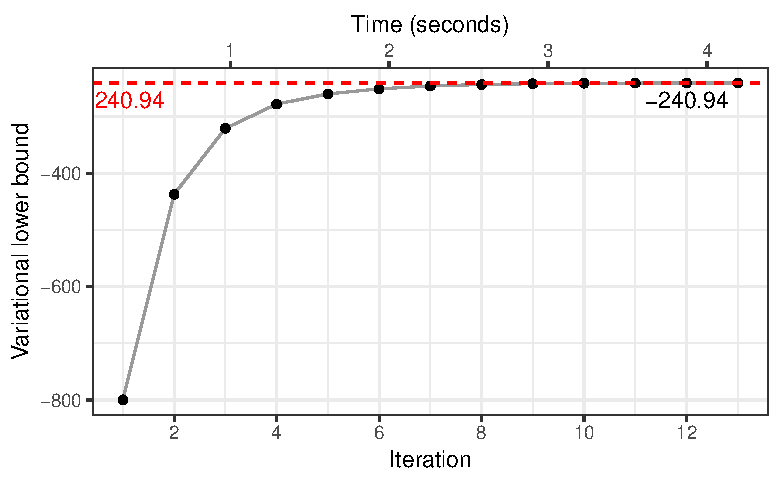
\includegraphics[width=0.785\linewidth]{figure/05-cardiac_mod_full_plot-1} 
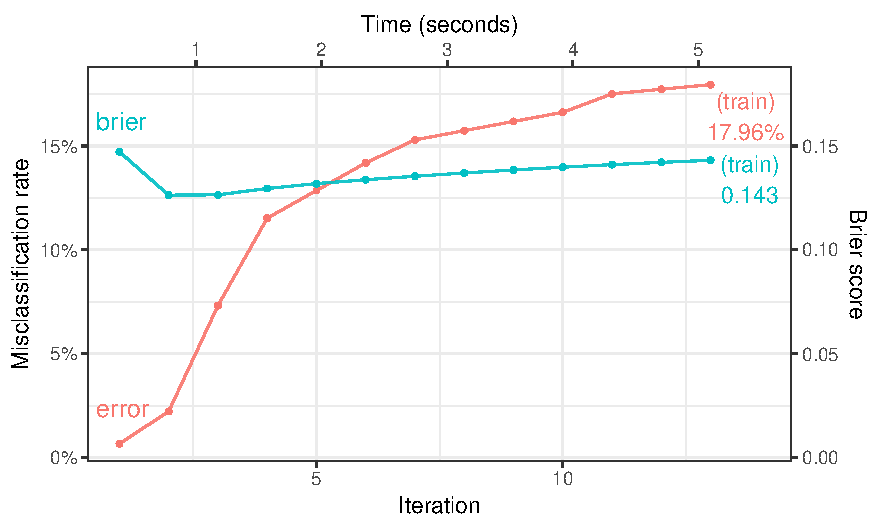
\includegraphics[width=0.785\linewidth]{figure/05-cardiac_mod_full_plot-2} 

}

\caption[Plot of variational lower bound over time (left), and plot of training error rate and Brier scores over time (right)]{Plot of variational lower bound over time (left), and plot of training error rate and Brier scores over time (right).}\label{fig:cardiac.mod.full.plot}
\end{figure}


\end{knitrout}

To measure predictive ability, we fit the I-probit models on a random subset of the data and obtain the out-of-sample test error rates from the remaining held-out observations.
We then compare the results against popular machine learning classifiers, namely: 1) linear and quadratic discriminant analysis (LDA/QDA); 2) $k$-nearest neighbours; 3) support vector machines (SVM) \citep{steinwart2008support}; 4) Gaussian process classification \citep{rasmussen2006gaussian}; 5) random forests \citep{breiman2001random}; 6) nearest shrunken centroids (NSC) \citep{tibshirani2002diagnosis}; and 7) L-1 penalised logistic regression \citep{friedman2001elements}.
The experiment is set up as follows:
\begin{enumerate}
  \item Form a training set by sub-sampling $s \in \{50, 100, 200\}$ observations.
  \item The remaining unsampled data is used as the test set.
  \item Fit model on training set, and obtain test error rates defined as
  \[
    \text{test error rate} = \frac{1}{s} \sum_{i=1}^n [y^{\text{pred}}_i \neq y^{\text{test}}_i] \times 100 \%.
  \]
  \item Repeat steps 1-3 100 times to obtain the \emph{average} test error rates and standard errors.
\end{enumerate}
Results for the methods listed above were extracted from the in-depth study by \citet{cannings2017random}, who also conducted identical experiments using their random projection (RP) ensemble classification method.
These are all tabulated in \cref{tab:cardiac}.

\begin{table}[htb]
  \caption[Mean out-of-sample misclassification rates and SE for the cardiac arrhythmia data set]{Mean out-of-sample misclassification rates and standard errors in parantheses for 100 runs of various training ($s$) and test ($451-s$) sizes for the cardiac arrhythmia binary classification task.}
  \label{tab:cardiac}
  \centering
  \begin{tabular}{l r r r}
  \toprule
  \Bot&\multicolumn{3}{ c }{{Misclassification rate (\%)}} \\
  \cline{2-4}
  \Top Method
  & {$s = 50$}
  & {$s = 100$}
  & {$s = 200$} \\
  \midrule
  \emph{I-probit} \\
  \hspace{0.5em} Linear            & 35.52 (0.44) & 31.35 (0.33) & 29.45 (0.38) \\
  \hspace{0.5em} Smooth (fBm-0.5)  & 33.64 (0.66) & 28.12 (0.34) & 24.33 (0.24) \\
  \hspace{0.5em} Smooth (SE-1.0)   & 48.26 (0.40) & 48.32 (0.43) & 47.11 (0.37) \\
  \\
  \emph{Others} \\
  \hspace{0.5em} RP-LDA            & 33.24 (0.42) & 30.19 (0.35) & 27.49 (0.30) \\
  \hspace{0.5em} RP-QDA            & 30.47 (0.33) & 28.28 (0.26) & 26.31 (0.28) \\
  \hspace{0.5em} RP-$k$-NN         & 33.49 (0.40) & 30.18 (0.33) & 27.09 (0.31)
  \\[0.5em]
  \hspace{0.5em} Random forests    & 31.65 (0.39) & 26.72 (0.29) & 22.40 (0.31) \\
  \hspace{0.5em} SVM (linear)      & 36.16 (0.47) & 35.61 (0.39) & 35.20 (0.35) \\
  \hspace{0.5em} SVM (Gaussian)    & 48.39 (0.49) & 47.24 (0.46) & 46.85 (0.43)
  \\[0.5em]
  \hspace{0.5em} GP (Gaussian)     & 37.28 (0.42) & 33.80 (0.40) & 29.31 (0.35) \\
  \hspace{0.5em} NSC               & 34.98 (0.46) & 33.00 (0.40) & 31.08 (0.41) \\
  \hspace{0.5em} L-1 logistic      & 34.92 (0.42) & 30.48 (0.34) & 26.12 (0.27) \\
  \end{tabular}
\end{table}

Of the three I-probit models, the fBm model performed the best.
That it performed better than the canonical linear I-probit model is unsurprising, since an underlying smooth function to model the latent variables is expected to generalise better than a rigid straight line function.
The poor performance of the SE I-probit model may be due to the fact that the lengthscale parameter was not estimated (fixed at $l=1$), but then again, we notice reliable performance of the fBm even with fixed Hurst index ($\gamma = 0.5$).
It can be seen that the fBm I-probit model also outperform the more popular machine learning algorithms out there including $k$-nearest neighbours, support vector machines and Gaussian process classification.
It came second only to random forests, an ensemble learning method, which is also generally faster to train than Gaussian process-like regressions such as I-prior models.
The time complexity of a random forest algorithm is $O(pqn\log(n))$ \citep{louppe2014understanding}, where $p$ is the number of variables used for training, $q$ is the number of random decision trees, and $n$ is the number of observations.

\subsection{Meta-analysis of smoking cessation}

Conider the smoking cessation data set, as described in \citet{skrondal2004generalized}.
It contains observations from 27 separate smoking cessation studies in which participants are subjected to either a nicotine gum treatment or a placebo.
The interest is to estimate the treatment effect size, and whether it is statistically significant, i.e. whether or not nicotine gum is an effective treatment for quitting smoking.
The studies are conducted at different times and due to various reasons such as funding and cultural effects, the results from all of the studies may not be in agreement.
The number of effective participants plays a major role in determining the power of the statistical tests performed in individual studies.
The question then becomes how do we meaningfully aggregate all the data to come up with one summary measure?

Several methods exist to analyse such data sets.
One may consider a fixed-effects model, similar to a classical one-way ANOVA model to establish whether or not the effect size is significant.
Because of the study-specific characteristics, it is natural to consider multilevel or random-effects models as a means to estimate the effect size.
Regardless of method, the approach of analysing study-level treatment effects instead of patient-level data only is the paradigm for meta-analysis, and our I-prior model takes this approach as well.
% However, analysing study-level estimates of effect size can be problematic for various reasons, such as small group samples or rare occurences.

\begin{knitrout}
\definecolor{shadecolor}{rgb}{1, 1, 1}\color{fgcolor}\begin{figure}[htb]

{\centering 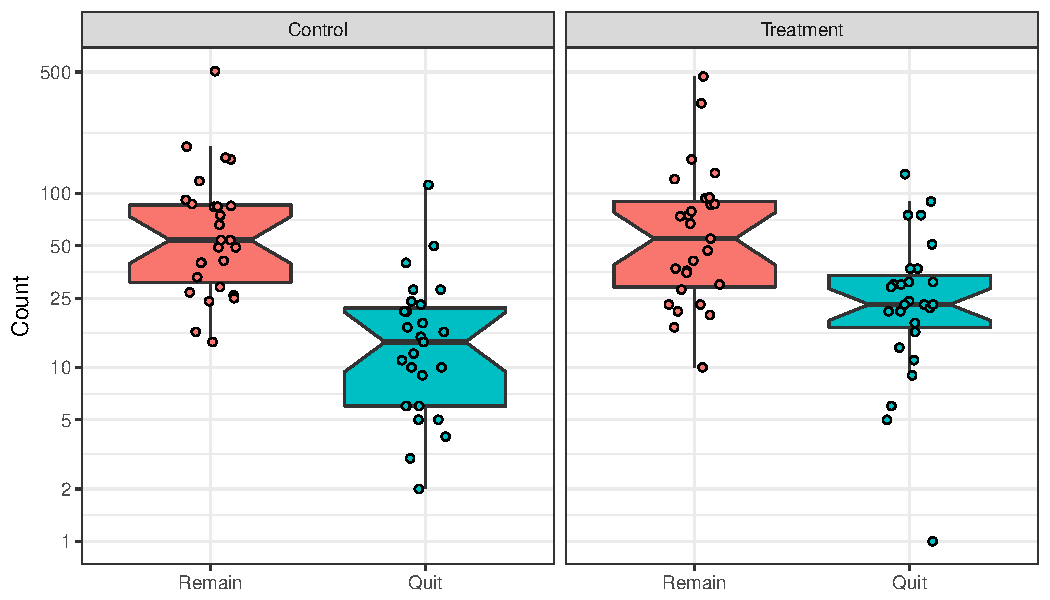
\includegraphics[width=\maxwidth]{figure/05-plot_data_smoke-1} 

}

\caption[Comparative box-plots of the distribution of patients who successfully quit smoking and those who remained smokers, in the two treatment groups]{Comparative box-plots of the distribution of patients who successfully quit smoking and those who remained smokers, in the two treatment groups. It is evident that there are more successful patients quitting smoking in the treatment group than in the control group. The raw odds ratio of quitting smoking (treatment vs. control) is 1.66.}\label{fig:plot.data.smoke}
\end{figure}


\end{knitrout}
A summary of the data is displayed by the box-plot in \cref{fig:plot.data.smoke}.
On the whole, there are a total of 5,908
% study.size[length(study.size)]
patients, and they are distributed roughly equally among the control and treatment groups (46.3\% and 53.7\% respectively, on average).
From the box-plots, it is evident that there are more patients who quit smoking in the treatment group as compared to the placebo control group.
There are various measures of treatment effect size, such as risk ratio or risk differences, but we shall concentrate on \emph{odds ratios} as defined by
\[
  \text{odds ratio} = \frac{\text{odds of quitting smoking in \emph{treatment} group}}
  {\text{odds of quitting smoking in \emph{control} group}}.
\]
The odds of quitting smoking in either group is defined as
\[
  \text{odds} = \frac{\Prob(\text{quit smoking})}{1 - \Prob(\text{quit smoking})},
\]
and these probabilities, odds and ultimately odds ratio can be estimated from sample proportions.
This raw odds ratio for all study groups is calculated as $1.66 = e^{0.50}$.
It is also common for the odds ratio to be reported on the log scale (usually as a remnant of logistic models).
A value greater than one for the odds ratio (or equivalently, greater than zero for the log odds ratio) indicates a significant treatment effect.

A random-effects analysis using a multilevel logistic model has been considered by \citet{agresti2000tutorial}.
Let $i=1,\dots,n_k$ index the patients in study group $k \in \{1,\dots,27\}$.
For patient $i$ in study $j$, $p_{ik}$ denotes the probability that the patient has successfully quit smoking.
Additionally, $x_{ik}$ is the centred dummy variable indicating patient $i$'s treatment group in study $k$.
These take on two values: 0.5 for treated patients and -0.5 for control patients.
The logistic random-effects model is
\begin{gather*}
  \log \left( \frac{p_{ij}}{1-p_{ij}} \right) = \beta_{0j} + \beta_{1j}x_{ij} \\
  \intertext{with}
  \begin{pmatrix} \beta_{0j} \\ \beta_{1j} \end{pmatrix}
  \sim \N \left(
  \begin{pmatrix} \beta_0 \\ \beta_1 \end{pmatrix},
  \begin{pmatrix} \sigma_0^2 & \sigma_{01} \\ \sigma_{01} & \sigma_1^2 \\ \end{pmatrix}
  \right)
\end{gather*}
\citet{agresti2000tutorial} also made the additional assumption $\sigma_{01} = 0$, so that, coupled with the contrast coding used for $x_{ik}$, the total variance $\Var(\beta_{0k} + \beta_{1j}x_{ik})$ would be constant in both treatment groups.
The overall log odds ratio is represented by $\beta_1$, and this is estimated as $0.57 \approx \log 1.76$.

In an I-prior model, the Bernoulli probabilities $p_{ik}$ are regressed against the treatment group indicators $x_{ik}$ and also the patients' study group $k$ via the regression function $f$ and a probit link:
\begin{align*}
  \Phi^{-1}(p_{ik})
  &= f(x_{ik}, k) \\
  &= f_1(x_{ik}) + f_2(k) + f_{12}(x_{ik}, j).
\end{align*}
We have decomposed our function $f$ into three parts: $f_1$ represents the treatment effect, $f_2$ represents the effect of the study groups, and $f_{12}$ represents the interaction effect between the treatment and study group on the modelled probabilities.
As both $x_{ik}$ and $k$ are nominal variables, the functions $f_1$ and $f_2$ both lie in the Pearson RKHS of functions $\cF_1$ and $\cF_2$, each with RKHS scale parameters $\lambda_1$ and $\lambda_2$.
As such, it does not matter how the $x_{ik}$ variables are coded (dummy coding 0, 1 vs. centred coding -0.5, 0.5) as the scaling of the function is determined by the RKHS scale parameters.
The interaction effect $f_{12}$ lies in the RKHS tensor product $\cF_1 \otimes \cF_2$.
In the I-probit model, there are only two parameters to estimate, while in the standard logistic random-effects model, there are six.
The results of the I-prior fit are summarised in the table below.


\newcolumntype{R}[1]{>{\raggedleft\arraybackslash}p{#1}}
\begin{table}[hbt]
  \centering
  \caption{Results of the I-probit model fit for three models.}
  \label{tab:mod.compare.smoke}
  \begin{tabular}{lrrrR{2cm}}
  \toprule
  Model & ELBO & Error rate (\%) & Brier score & No. of parameters \\
  \midrule
  $f_1$
  &-3210.76
  &23.65
  &0.179 & 1 \\
  $f_1+f_2$
  &-3142.24
  &29.30
  &0.206 & 2 \\
  $f_1+f_2+f_{12}$
  &-3091.20
  &23.48
  &0.168 & 2 \\
  \bottomrule
  \end{tabular}
\end{table}

The approximated marginal log-likelihood value for the I-prior model (i.e. variational lower bound), the Brier score for each model and the number of RKHS scale parameters estimated in the model are reported in \cref{tab:mod.compare.smoke}. Three models were fitted:
1) a model with only the treatment effect;
2) a model with a treatment effect and a study group effect; and
3) Model 2 with the additional assumption that treatment effect varies across study groups.
Model 1 disregards the study group effects, while Model 2 assumes that the effectiveness of the nicotine gum treatment does not vary across study groups (akin to a varying-intercept model).
A model comparison using the evidence lower bound indicates that Model 3 has the highest value, and the difference is significant from a Bayes factor standpoint---$\BF(M_3,M_1)$ and $\BF(M_3,M_2)$ are both greater than 150.
% with both Bayes factor comparing Model 3 against Models 1 and 2 being greater than 150.
% $\BF(M_3, M_1)iprior::dec_plac(exp(l[3] - l[1]), 2)$ and $\BF(M_3, M_2)iprior::dec_plac(exp(l[3] - l[2]), 2)$.
% Although not soundly based in theory, we may compare variational lower bounds of the three models for model selection as a proxy to using the true log-likelihood value.
% In this case, Model 3 has the highest lower bound value.
The misclassification rate and Brier score indicates good predictive performance of the models, and there is not much to distinguish between the three although Model 3 is the best out of the three models.

\begin{knitrout}
\definecolor{shadecolor}{rgb}{1, 1, 1}\color{fgcolor}\begin{figure}[p]

{\centering 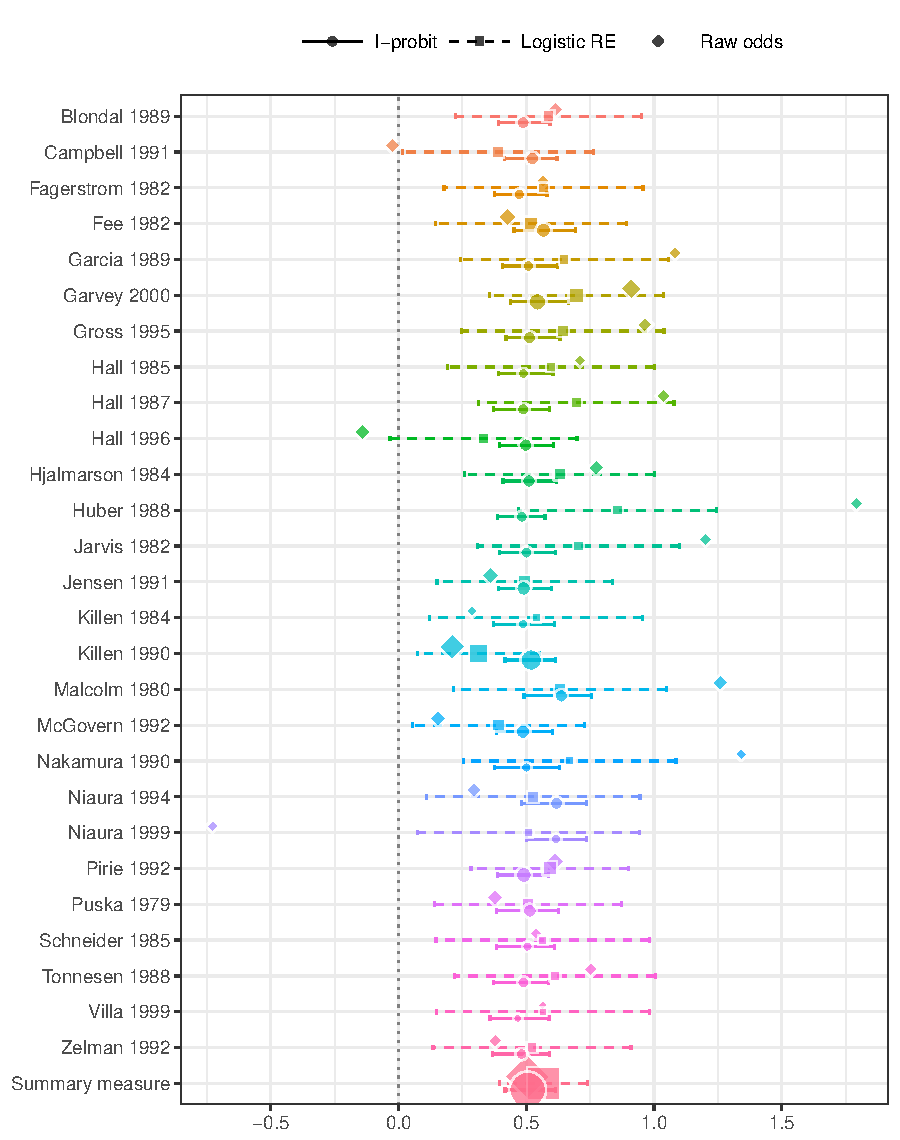
\includegraphics[width=\linewidth]{figure/05-smoke_forest_plot-1} 

}

\caption[Forest plot of effect sizes (log odds ratios) in each group as well as the overall effect size together with their 95\% confidence bands]{Forest plot of effect sizes (log odds ratios) in each group as well as the overall effect size together with their 95\% confidence bands. The plot compares the raw log odds ratios, the logistic random-effect estimates, and the I-prior estimates. Sizes of the points indicate the relative sample sizes per study group.}\label{fig:smoke.forest.plot}
\end{figure}


\end{knitrout}

Unlike in the logistic random-effects model, where the log odds ratio can be read off directly from the coefficients, with an I-prior probit model the log odds ratio needs to be calculated manually from the fitted probabilities.
The probabilities of interest are the probabilities of quitting smoking under each treatment group for each study group $k$---call these $p_k(\text{treatment})$ and $p_k(\text{control})$.
That is,
\begin{align*}
  p_k(\text{treatment}) &= \Phi\big( \hat\nu(\text{treatment}, k) \big) \\
  p_k(\text{control})   &= \Phi\big( \hat\nu(\text{control}, k) \big),
\end{align*}
where $\hat \nu$ represents the standardised posterior mean estimate for the regression functions which are distributed according to
\[
  f(x_{ik},k)|\by,\hat\theta \sim \N\big(\hat\mu(x_{ik}, k), \hat\sigma^2(x_{ij}, k) \big),
\]
with $x_{ik}\in\{\text{treatment}, \text{control} \}$ and $k \in \{1,\dots,27\}$  (see details in \cref{sec:iprobitpostest}).
The log odds ratio for each study group can then be calculated as usual.
For the overall log odds ratio, the probabilities that are used are the averaged probabilities weighted according to the sample sizes in each group.
This has been calculated as $0.51 \approx \log 1.66$, slightly lower than both the raw log odds ratio and the log odds ratio estimated by the logistic random-effects model.
This can perhaps be attributed to some shrinkage of the estimated probabilities due to placing a prior with zero mean on the regression functions.

The credibility intervals for the log odds ratios in the forest plot of \cref{fig:smoke.forest.plot} are also noticeably narrower under an I-prior compared to the fitted multilevel model.
One explanation is that empirical Bayes estimates, such as the I-probit estimates under a variational EM framework, tend to underestimate the variability in the estimates because the variability in the parameters are ignored when point estimates are used, compared to distributions in a true Bayesian estimation framework.

\subsection{Multiclass classification: Vowel recognition data set}





We illustrate multiclass classification using I-priors on a speech recognition data set\footnotemark~with $m = 11$ classes to be predicted from digitized low pass filtered signals generated from voice recordings.
Each class corresponds to a vowel sound made when pronouncing a specific word.
The words that make up the vowel sounds are shown in \cref{tab:vowel}. Each word was uttered once by multiple speakers, and the data are split into a training and a test set.
Four males and four female speakers contributed to the training set, while four male and three female speakers contributed to the test set.
The recordings were manipulated using speech processing techniques, such that each speaker yielded six frames of speech from the eleven vowels, each with a corresponding 10-dimensional numerical input vector (the predictors).
This means that the size of the training set is $8 \times 6 \times 11 = 528$, while $7 \times 6 \times 11 = 462$ data points are available for testing the predictive performance of the models.
This data set is also known as Deterding's vowel recognition data (after the original collector, \cite{deterding1989speaker}).
Machine learning methods such as neural networks and nearest neighbour methods were analysed by \citet{robinson1989dynamic}.

\footnotetext{Data is publicaly available from the UCI Machine Learning Repository, URL: \url{https://archive.ics.uci.edu/ml/datasets/Connectionist+Bench+(Vowel+Recognition+-+Deterding+Data)}.}

\begin{table}[htb]
\centering
\caption{The eleven words that make up the classes of vowels.}
\label{tab:vowel}
\begin{tabular}{llllllllll}
\toprule
Class & Label          & Vowel & Word &  && Class & Label          & Vowel & Word  \\
\midrule
1     & \texttt{hid} & \dsil{iː}    & heed &&  & 7     & \texttt{hOd} & \dsil{ɒ}    & hod   \\
2     & \texttt{hId} & \dsil{ɪ}     & hid  &&  & 8     & \texttt{hod} & \dsil{ɔː}   & hoard \\
3     & \texttt{hEd} & \dsil{ɛ}     & head &&  & 9     & \texttt{hUd} & \dsil{ʊ}    & hood  \\
4     & \texttt{hAd} & \dsil{a}     & had  &&  & 10    & \texttt{hud} & \dsil{uː}   & who'd \\
5     & \texttt{hYd} & \dsil{ʌ}     & hud  &&  & 11    & \texttt{hed} & \dsil{əː}   & heard \\
6     & \texttt{had} & \dsil{ɑː}    & hard &&  &       &              &             &       \\
\bottomrule
\end{tabular}
\end{table}

We will fit the data using an I-probit model with the canonical linear kernel, fBm-0.5 kernel, and the SE kernel with lengthscale $l=1$.
% We assume $m = 11$ distinct I-priors corresponding to the latent variables in each class, thus there are 11 unique intercepts and 11 RKHS scale parameters to estimate in each model.
Each model took roughly 13 seconds per iteration in fitting the training data set ($n=528$).
In particular, the canonical kernel model took a long time to converge, with each variational inference iteration improving the lower bound only slighly each time.
In contrast, both the fBm-0.5 and SE model were quicker to converge.
Multiple restarts from different random seeds were conducted, and we found that they all converged to a similar lower bound value.
This alleviates any concerns that the model might have converged to different multiple local optima.

\begin{knitrout}
\definecolor{shadecolor}{rgb}{1, 1, 1}\color{fgcolor}\begin{figure}[htb]

{\centering \subfloat[Canonical kernel\label{fig:vowel.confusion.matrix1}]{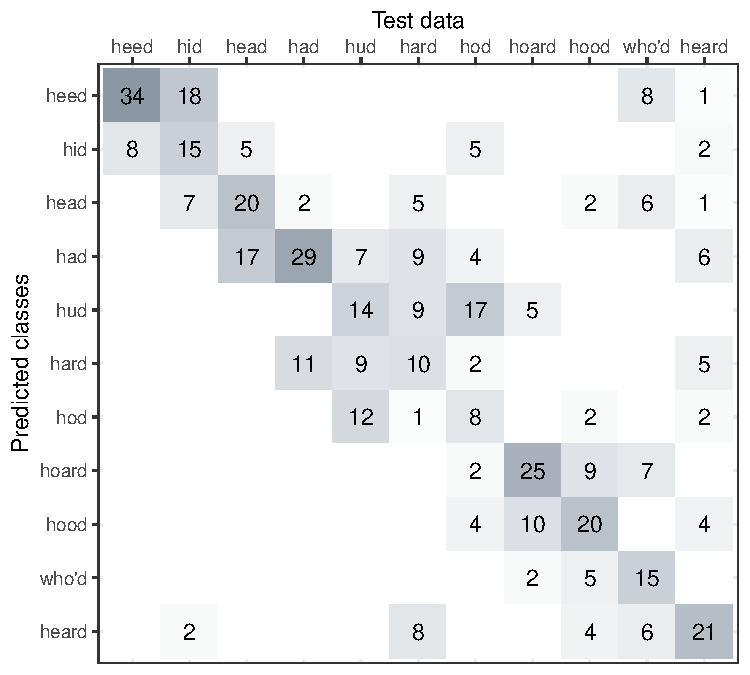
\includegraphics[width=0.485\linewidth]{figure/05-vowel_confusion_matrix-1} }
\subfloat[fBm-0.5 kernel\label{fig:vowel.confusion.matrix2}]{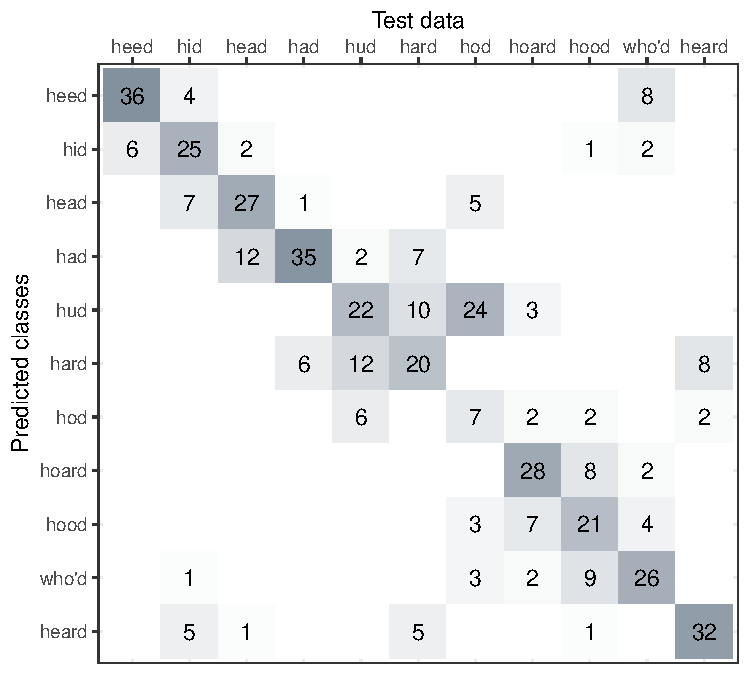
\includegraphics[width=0.485\linewidth]{figure/05-vowel_confusion_matrix-2} }
\subfloat[SE kernel\label{fig:vowel.confusion.matrix3}]{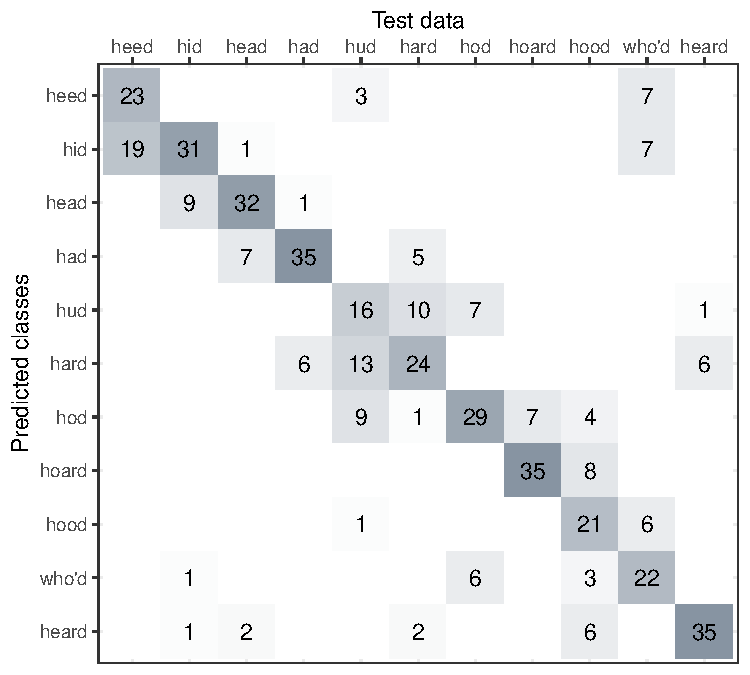
\includegraphics[width=0.485\linewidth]{figure/05-vowel_confusion_matrix-3} }

}

\caption[Confusion matrices for the vowel classification problem in which predicted values were obtained from the I-probit models]{Confusion matrices for the vowel classification problem in which predicted values were obtained from the I-probit models. The maximum value for any cell is 42 (seven speakers delivered six frames of speech per vowel). Blank cells indicate nil values.}\label{fig:vowel.confusion.matrix}
\end{figure}


\end{knitrout}

A good way to visualise the performance of model predictions is through a confusion matrix, as shown in \cref{fig:vowel.confusion.matrix}.
The numbers in each row indicate the instances of a predicted class, while the numbers in the column indicate instances of the actual classes, while nil values are indicated by blank cells.
% A quick glance of the plots seem to favour the fBm-0.5 kernel as having better predictions.
% There are a lot more misclassifications when using the canonical kernel.
% Under the fBm-0.5 model, the model makes understandable mistakes - confusing very similar words, especially `hod' and `hud'.

Comparisons to other methods that had been used to analyse this data set is given in \cref{tab:vowel.tab}.
In particular, the I-probit model is compared against 1) linear regression; 2) logistic linear regression; 3) linear and quadratic discriminant analysis; 4) decision trees; 5) neural networks; 6) $k$-nearest neighbours; and 7) flexible discriminant analysis.
All of these methods are described in further detail in \citet[Ch.4 \& 12, Table 12.3]{friedman2001elements}.
The I-probit model using both the fBm-0.5 and SE kernel offers one of the best out-of-sample classification error rates (34.4\%) of all the methods compared.
The linear I-probit model is seen to be comparable to logistic regression, linear and quadratic discrimant analysis, and also decision trees.
It also provides significant improvement over multiple linear regression.

\begin{table}
  \caption{Results of various classification methods for the vowel data set.}
  \label{tab:vowel.tab}
  \centering
  \begin{tabular}{l r r}
  \toprule
  \Bot &\multicolumn{2}{c}{Error rate (\%)} \\
  \cline{2-3}
  \Top Model & Train & Test \\
  \midrule
  \emph{I-probit} \\
  \hspace{0.5em} Linear
  & 29
  & 54 \\
  \hspace{0.5em} Smooth (fBm-0.5)
  & 22
  & 40 \\
  \hspace{0.5em} Smooth (SE-1.0)
  & 7
  & 34 \\
  \\
  \emph{Others} \\
  \hspace{0.5em} Linear regression               & 48 & 67 \\
  \hspace{0.5em} Logistic regression             & 22 & 51
  \\[0.5em]
  \hspace{0.5em} Linear discriminant analysis    & 32 & 56 \\
  \hspace{0.5em} Quadratic discriminant analysis & 1  & 53
  \\[0.5em]
  \hspace{0.5em} Decision trees                  & 5  & 54 \\
  \hspace{0.5em} Neural networks                 &    & 45 \\
  \hspace{0.5em} $k$-nearest neighbours          &    & 44
  \\[0.5em]
  \hspace{0.5em} FDA/BRUTO                       & 6  & 44 \\
  \hspace{0.5em} FDA/MARS                        & 13 & 39 \\
  \bottomrule
  \end{tabular}
\end{table}

\subsection{Spatio-temporal modelling of bovine tuberculosis in Cornwall}



Data containing the number of breakdows of bovine tubercolosis (BTB) in Cornwall, the locations of the infected animals, and the year of occurence is analysed.
The interest, as motivated by veterinary epidimiology, is to understand whether or not there is spatial segregation of the infection of the herds, and whether there is a time-element to the presence or absence of this spatial segregation.
There has been previous work done to analyse this data set.
\citet{diggle2005nonparametric} developed a non-parametric method to estimate spatial segregation using a multivariate point process.
The occurrences are modelled as Poisson point processes, and spatial segregation is said to have occured if the model-estimated type-specific breakdown probabilities at any given location are not significantly different from the sample proportions.
The authors estimated the probabilities via kernel regression, and the test statistic of interest had to be estimated via Monte Carlo methods.
Other works include \citet{diggle2013spatial}, who used a fully Bayesian approach for spatio-temporal multivariate log-Gaussian Cox processes, which is implemented in the \proglang{R} package \pkg{lgcp} \citep{taylor2013lgcp}.

\begin{knitrout}
\definecolor{shadecolor}{rgb}{1, 1, 1}\color{fgcolor}\begin{figure}[htb]

{\centering 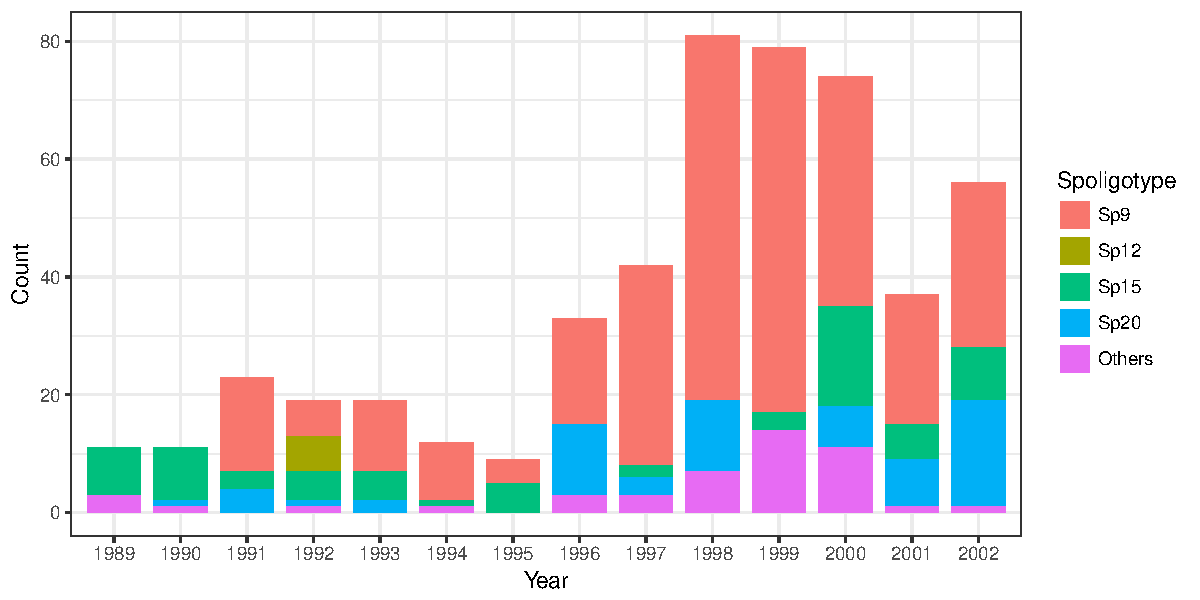
\includegraphics[width=\linewidth]{figure/05-plot_cow-1} 

}

\caption[Distribution of the different types (Spoligotypes) of bovine tubercolosis affecting herds in Cornwall over the period 1989 to 2002]{Distribution of the different types (Spoligotypes) of bovine tubercolosis affecting herds in Cornwall over the period 1989 to 2002.}\label{fig:plot.cow}
\end{figure}


\end{knitrout}

The data set contains $n=919$ recorded cases over a span of 14 years.
For each of the cases, spatial data pertaining to the location of the farm (Northings and Eastings, measured in kilometres) are available.
Originally, 11 unique spoligotypes were recorded in the data, with the four most common spoligotypes being Sp9 ($m=1$), Sp12 ($m=2$), Sp15 ($m=3$) and Sp20 ($m=4$), as shown by the histogram in \cref{fig:plot.cow}.
We had grouped the remaining seven spoligotypes into an `Others' category ($m=5$), so that the problem becomes a multinomial regression with five distinct outcomes.

\begin{knitrout}
\definecolor{shadecolor}{rgb}{1, 1, 1}\color{fgcolor}\begin{figure}[htb]

{\centering 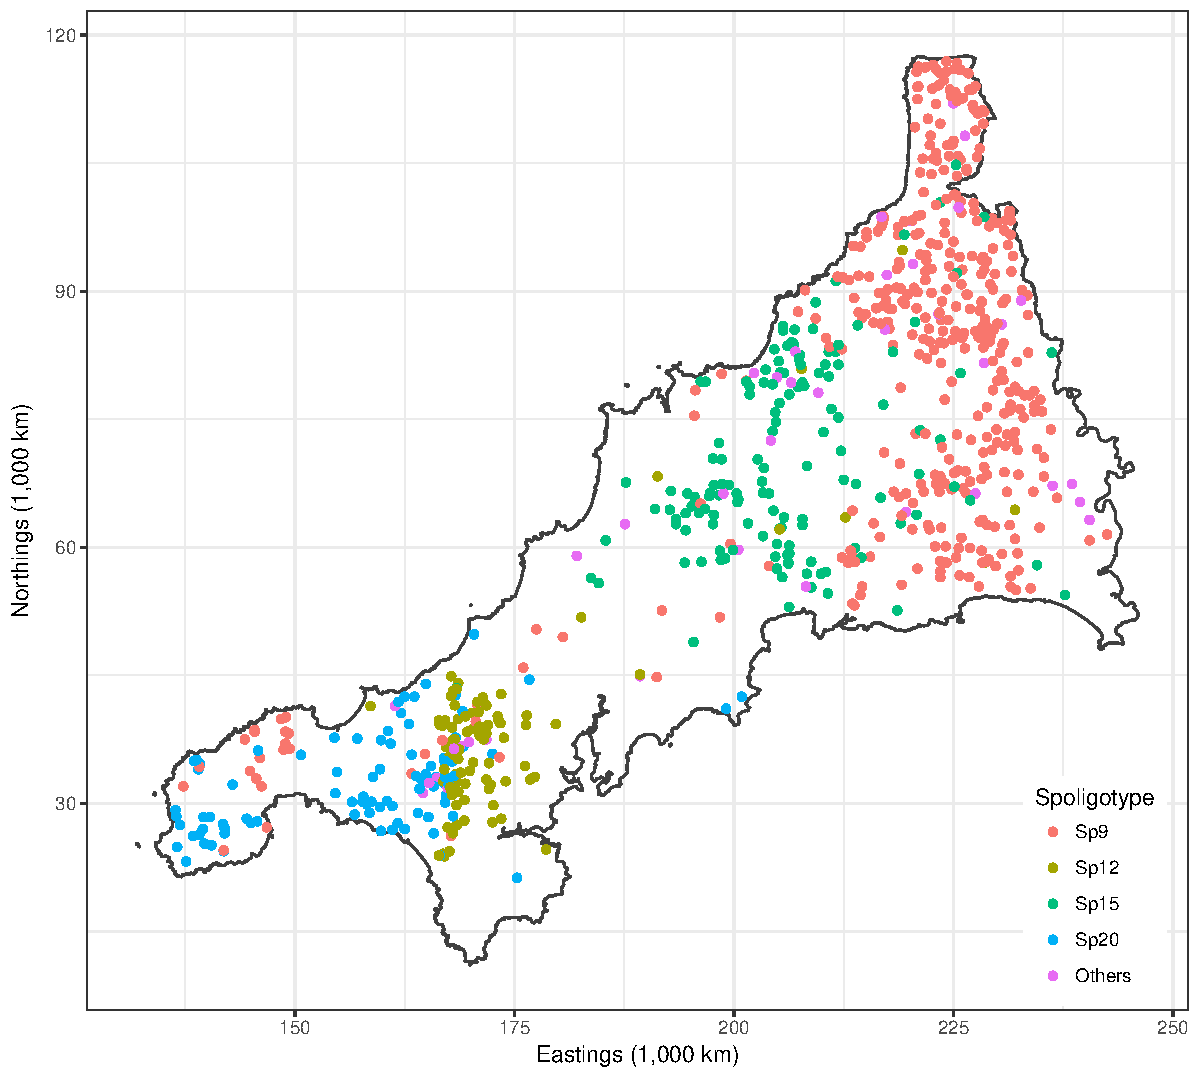
\includegraphics[width=\linewidth]{figure/05-plot_cornwall-1} 

}

\caption[Spatial distribution of all cases over the 14 years]{Spatial distribution of all cases over the 14 years.}\label{fig:plot.cornwall}
\end{figure}


\end{knitrout}

We are able to investigate any spatio-temporal patterns of infection using I-priors rather simply.
Let $p_{ij}$ denote the probability that a particular farm $i$ is infected with a BTB disease with spoligotype $j \in \{1,\dots,5\}$.
We model the transformed probabilities $g_j(p_{ij})$ as following a function which takes two covariates, i.e. the spatial data $x_1 \in \bbR^2$, and the temporal data $x_2$ (year of infection):
\begin{align*}
  p_{ij}
  &= g_j^{-1} \big( f_k(x_1, x_2) \big)_{k=1}^m \\
  &= g_j^{-1} \big( f_{1k}(x_1) + f_{2k}(x_2) + f_{12k}(x_1, x_2) \big)_{k=1}^m,
\end{align*}
where the function $g_j^{-1}:\bbR^m \to [0,1]$ is the same squashing function used in equation \cref{eq:intractablelikelihood2}.
We assume a smooth effect of space and time on the probabilities, and appropriate RKHSs for the functions $f_1 \in \cF_1$ and $f_2 \in \cF_2$ are the fBm-0.5 RKHS.
Alternatively, as per \citet{diggle2005nonparametric}, divide the data into four distinct time periods:
1) 1996 and earlier;
2) 1997 to 1998;
3) 1999 to 2000;
and finally 4) 2001 to 2002.
In this case, $x_2$ would indicate which period the infection took place in, and thus would have a nominal effect on the probabilities.
An appropriate RKHS for $f_2$ in such a case would be the Pearson RKHS.
In either case, the function $f_{12} \in \cF_1 \otimes \cF_2$ would be the ``interaction effect'', meaning that with such an effect present, the spatial distribution of the diseases are assumed to vary across the years.

\begin{sidewaystable}[p]
\caption[Results of the fitted I-probit models for the BTB data set]{\label{tab:table.btb}Results of the fitted I-probit models. Estimates of the class intercepts and scale parameters, together with their respective bootstrap standard errors, are presented. For model comparison, we can look at ELBOs, error misclassification rates, and Brier scores.}
\centering
\begin{tabular}[t]{lrrrrrrrrrrr}
\toprule
\multicolumn{1}{c}{ } & \multicolumn{2}{r}{$M_0$: Intercepts only} & \multicolumn{1}{c}{ } & \multicolumn{2}{r}{$M_1$: Spatial only} & \multicolumn{1}{c}{ } & \multicolumn{2}{r}{$M_2$: Spatio-temporal} & \multicolumn{1}{c}{ } & \multicolumn{2}{r}{$M_3$: Spatio-period} \\
\cmidrule(l{2pt}r{2pt}){2-3} \cmidrule(l{2pt}r{2pt}){5-6} \cmidrule(l{2pt}r{2pt}){8-9} \cmidrule(l{2pt}r{2pt}){11-12}
  & Estimate & S.E. &   & Estimate & S.E. &   & Estimate & S.E. &   & Estimate & S.E.\\
\midrule
Intercept (Sp9) & 0.948 & 0.000 &  & 1.364 & 0.015 &  & 1.401 & 0.079 &  & 1.395 & 0.103\\
Intercept (Sp12) & -0.173 & 0.000 &  & -0.435 & 0.013 &  & -0.506 & 0.017 &  & -0.463 & 0.045\\
Intercept (Sp15) & 0.103 & 0.000 &  & -0.020 & 0.011 &  & -0.008 & 0.059 &  & -0.010 & 0.094\\
Intercept (Sp20) & -0.202 & 0.000 &  & -0.775 & 0.051 &  & -0.795 & 0.223 &  & -0.783 & 0.343\\
Intercept (Others) & -0.676 & 0.000 &  & -0.134 & 0.016 &  & -0.091 & 0.077 &  & -0.139 & 0.104\\[0.5em]
Scale (spatial) &  &  &  & 0.194 & 0.008 &  & -0.176 & 0.178 &  & 0.172 & 0.169\\
Scale (temporal) &  &  &  &  &  &  & -0.006 & 0.003 &  & -0.004 & 0.006\\
\\
ELBO & -1187.47 &  &  & -564.33 &  &  & -537.23 &  &  & -543.94 & \\
Error rate (\%) & 46.25 &  &  & 19.26 &  &  & 18.06 &  &  & 18.50 & \\
Brier score & 0.249 &  &  & 0.143 &  &  & 0.136 &  &  & 0.138 & \\
\bottomrule
\end{tabular}
\end{sidewaystable}

We fitted four different models:
\begin{itemize}
  \item \textbf{\boldmath$M_0$: Intercept only}.
  \[
    p_{ij} = g^{-1}_j\big( \alpha_k \big)_{k=1}^m
  \]
  \item \textbf{\boldmath$M_1$: Spatial segregation}.
  \[
    p_{ij} = g^{-1}_j\big(\alpha_k + f_{1k}(x_i) \big)_{k=1}^m
  \]
  $f_{1k} \in \cF_1$ Pearson RKHS.
  \item \textbf{\boldmath$M_2$: Spatio-temporal}.
  \[
    p_{ij} = g^{-1}_j\big(\alpha_k + f_{1k}(x_i) + f_{2k}(t_i) + f_{12k}(x_i,t_i) \big)_{k=1}^m
  \]
  $f_{1k} \in \cF_1$ Pearson RKHS, $f_{2k} \in \cF_2$ fBm-0.5 RKHS, and $f_{12k} \in \cF_1\otimes\cF_2$
  \item \textbf{\boldmath$M_3$: Spatio-period}.
  \[
    p_{ij} = g^{-1}_j\big(\alpha_k + f_{1k}(x_i) + f_{2k}(t_i) + f_{12k}(x_i,t_i) \big)_{k=1}^m
  \]
  $f_{1k} \in \cF_1$ Pearson RKHS, $f_{2k} \in \cF_2$ Pearson RKHS, and $f_{12k} \in \cF_1\otimes\cF_2$
\end{itemize}
Model $M_0$ corresponds to a model which ignores any spatial or temporal effects (the baseline intercept only model).
Model $M_1$ takes into account only spatial effects.
Both models $M_2$ and $M_3$ account for spatio-temporal effects, but $M_2$ assumes a smooth effect of time, while $M_3$ segregates the points into four distinct time periods for analysis.
Model comparison is easily done, and \cref{tab:table.btb} indicates that model $M_2$ has the highest log-likelihood of the four models, making it the preferable model.

% Alternatively, spatio-temporal effects of the BTB breakdowns can easily be inferred through the RKHS scale parameters.
% Let $h_k$, $k \in \{1,2\}$ denote the reproducing kernel of the spatial and temporal RKHSs respectively.
% Then, an I-prior on $f_j = f_{1j} + f_{2j} + f_{12j}$, $j=1,\dots,5$, takes the form
% \[
%   f_j(x_1,x_2) = \sum_{i=1}^n \big(
%   \lambda_1 h_1(x_1, x_{i1}) + \lambda_2 h_2(x_2, x_{i2}) +
%   \lambda_1\lambda_2 h_1(x_1, x_{i1}) h_2(x_2, x_{i2})
%   \big)w_{ij}
% \]
% where it is assumed $(w_{i1},\dots,w_{i5})^\top \iid \N(\bzero,\bI_5)$.
% The hypothesis of temporal significance is the same as testing the significance of the $\lambda_2$ parameter, while the test of both spatial and temporal effects are conducted on $\lambda_1$ and $\lambda_2$ simultaneously.
% From \hltodo{Chapter X}, we know that these scale parameters follow a normal posterior distribution, so we can calculate the $Z$-scores by dividing the mean by its corresponding standard deviation.
% Absolute values greater than three would satisfy a Bayesian hypothesis test of significance at the 0.01 level.
% The conclusion from \cref{tab:table.btb} is that the data supports a hypothesis for a spatio-temporal or spatio-period model.

For a more visual approach, we can look at the plots of the surface probabilities.
To obtain these probabilities, we first determined the spatial points (Northings and Eastings) which fall inside the polygon which makes up Cornwall.
We then obtained predicted probabilities for each class of disease at each location.
\cref{fig:plot.btb} was obtained using the model with spatial covariates only, thus ignoring any temporal effects.
In the case of the spatio-temporal model, we used the model which had the period formulation for time (model $M_3$).
This way, we can display the surface probabilities of the time periods in four plots only, which is more economical to exhibit within the margins of this thesis.
Note that there is no issue with using the continuous time model---we have produced an animated gif image at \url{http://phd.haziqj.ml/examples/}, showing the evolution of the surface probabilities over time.

\begin{knitrout}
\definecolor{shadecolor}{rgb}{1, 1, 1}\color{fgcolor}\begin{figure}[p]

{\centering 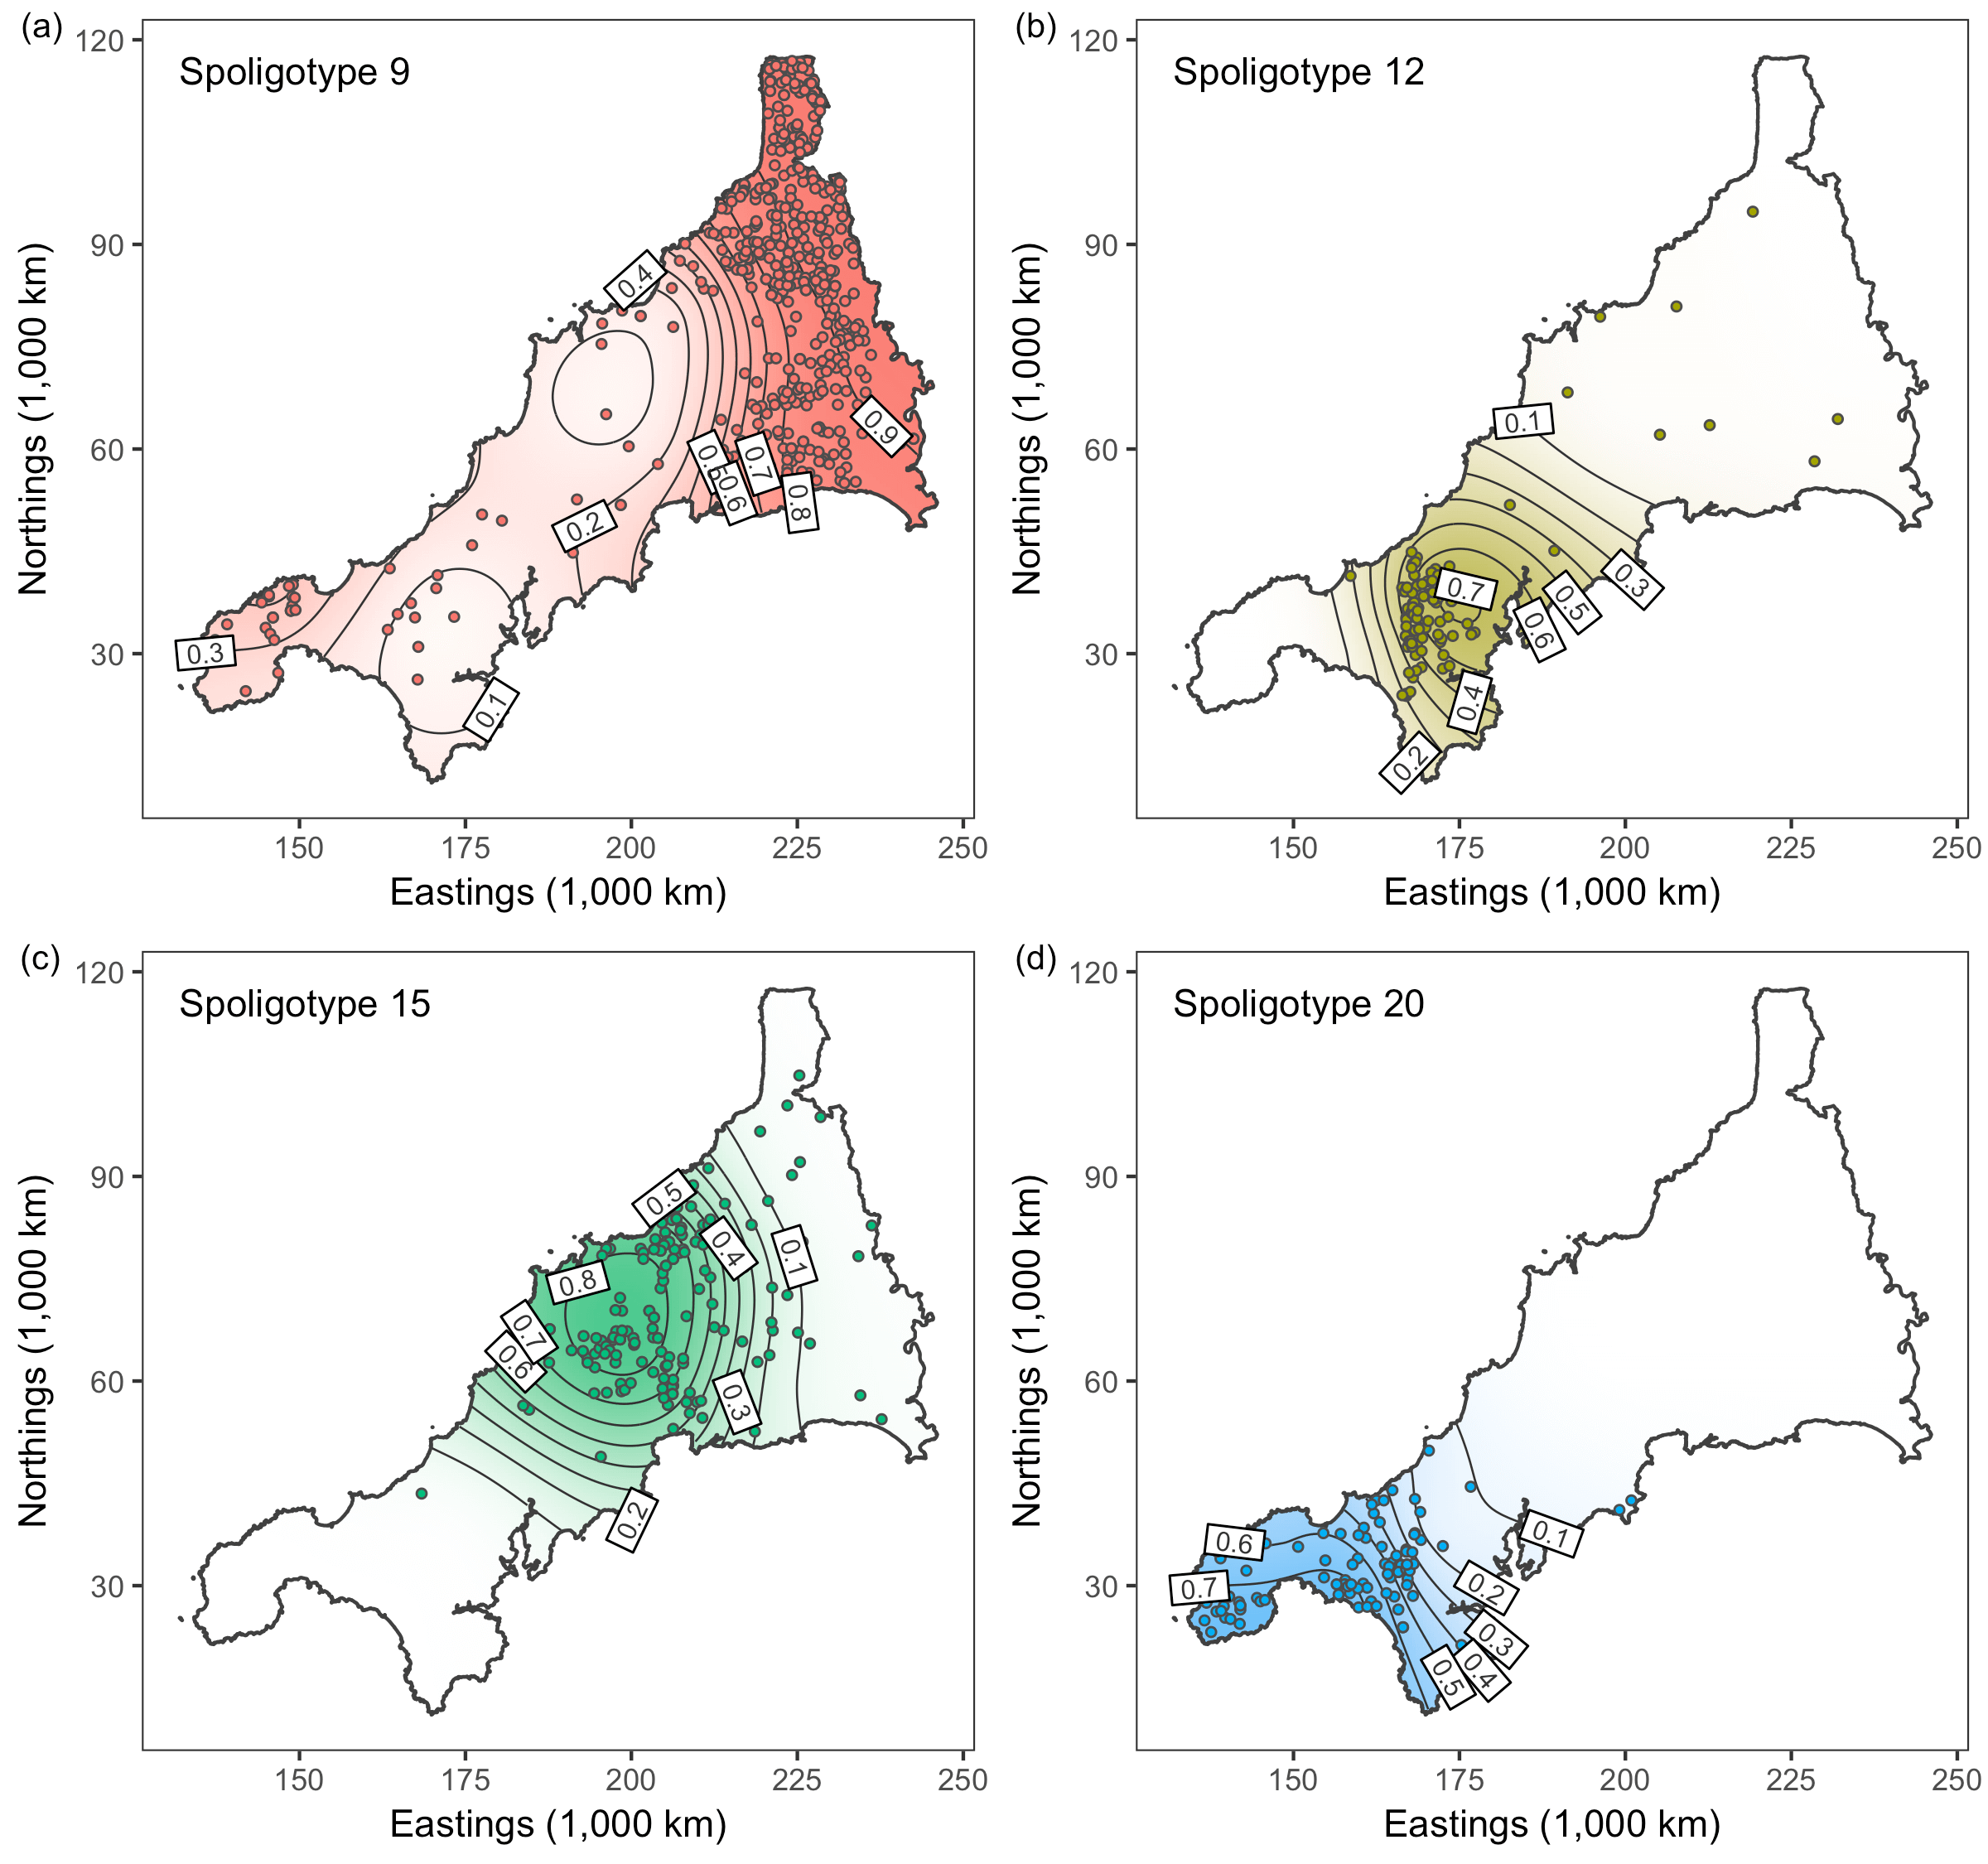
\includegraphics[width=\linewidth]{figure/05-plot_btb-1} 

}

\caption[Predicted probability surfaces for BTB contraction in Cornwall for the four largest spoligotypes of the bacterium \emph{Mycobacterium bovis} over the entire time period using model $M_1$]{Predicted probability surfaces for BTB contraction in Cornwall for the four largest spoligotypes of the bacterium \emph{Mycobacterium bovis} over the entire time period using model $M_1$.}\label{fig:plot.btb}
\end{figure}


\end{knitrout}
\begin{knitrout}
\definecolor{shadecolor}{rgb}{1, 1, 1}\color{fgcolor}\begin{figure}[p]

{\centering 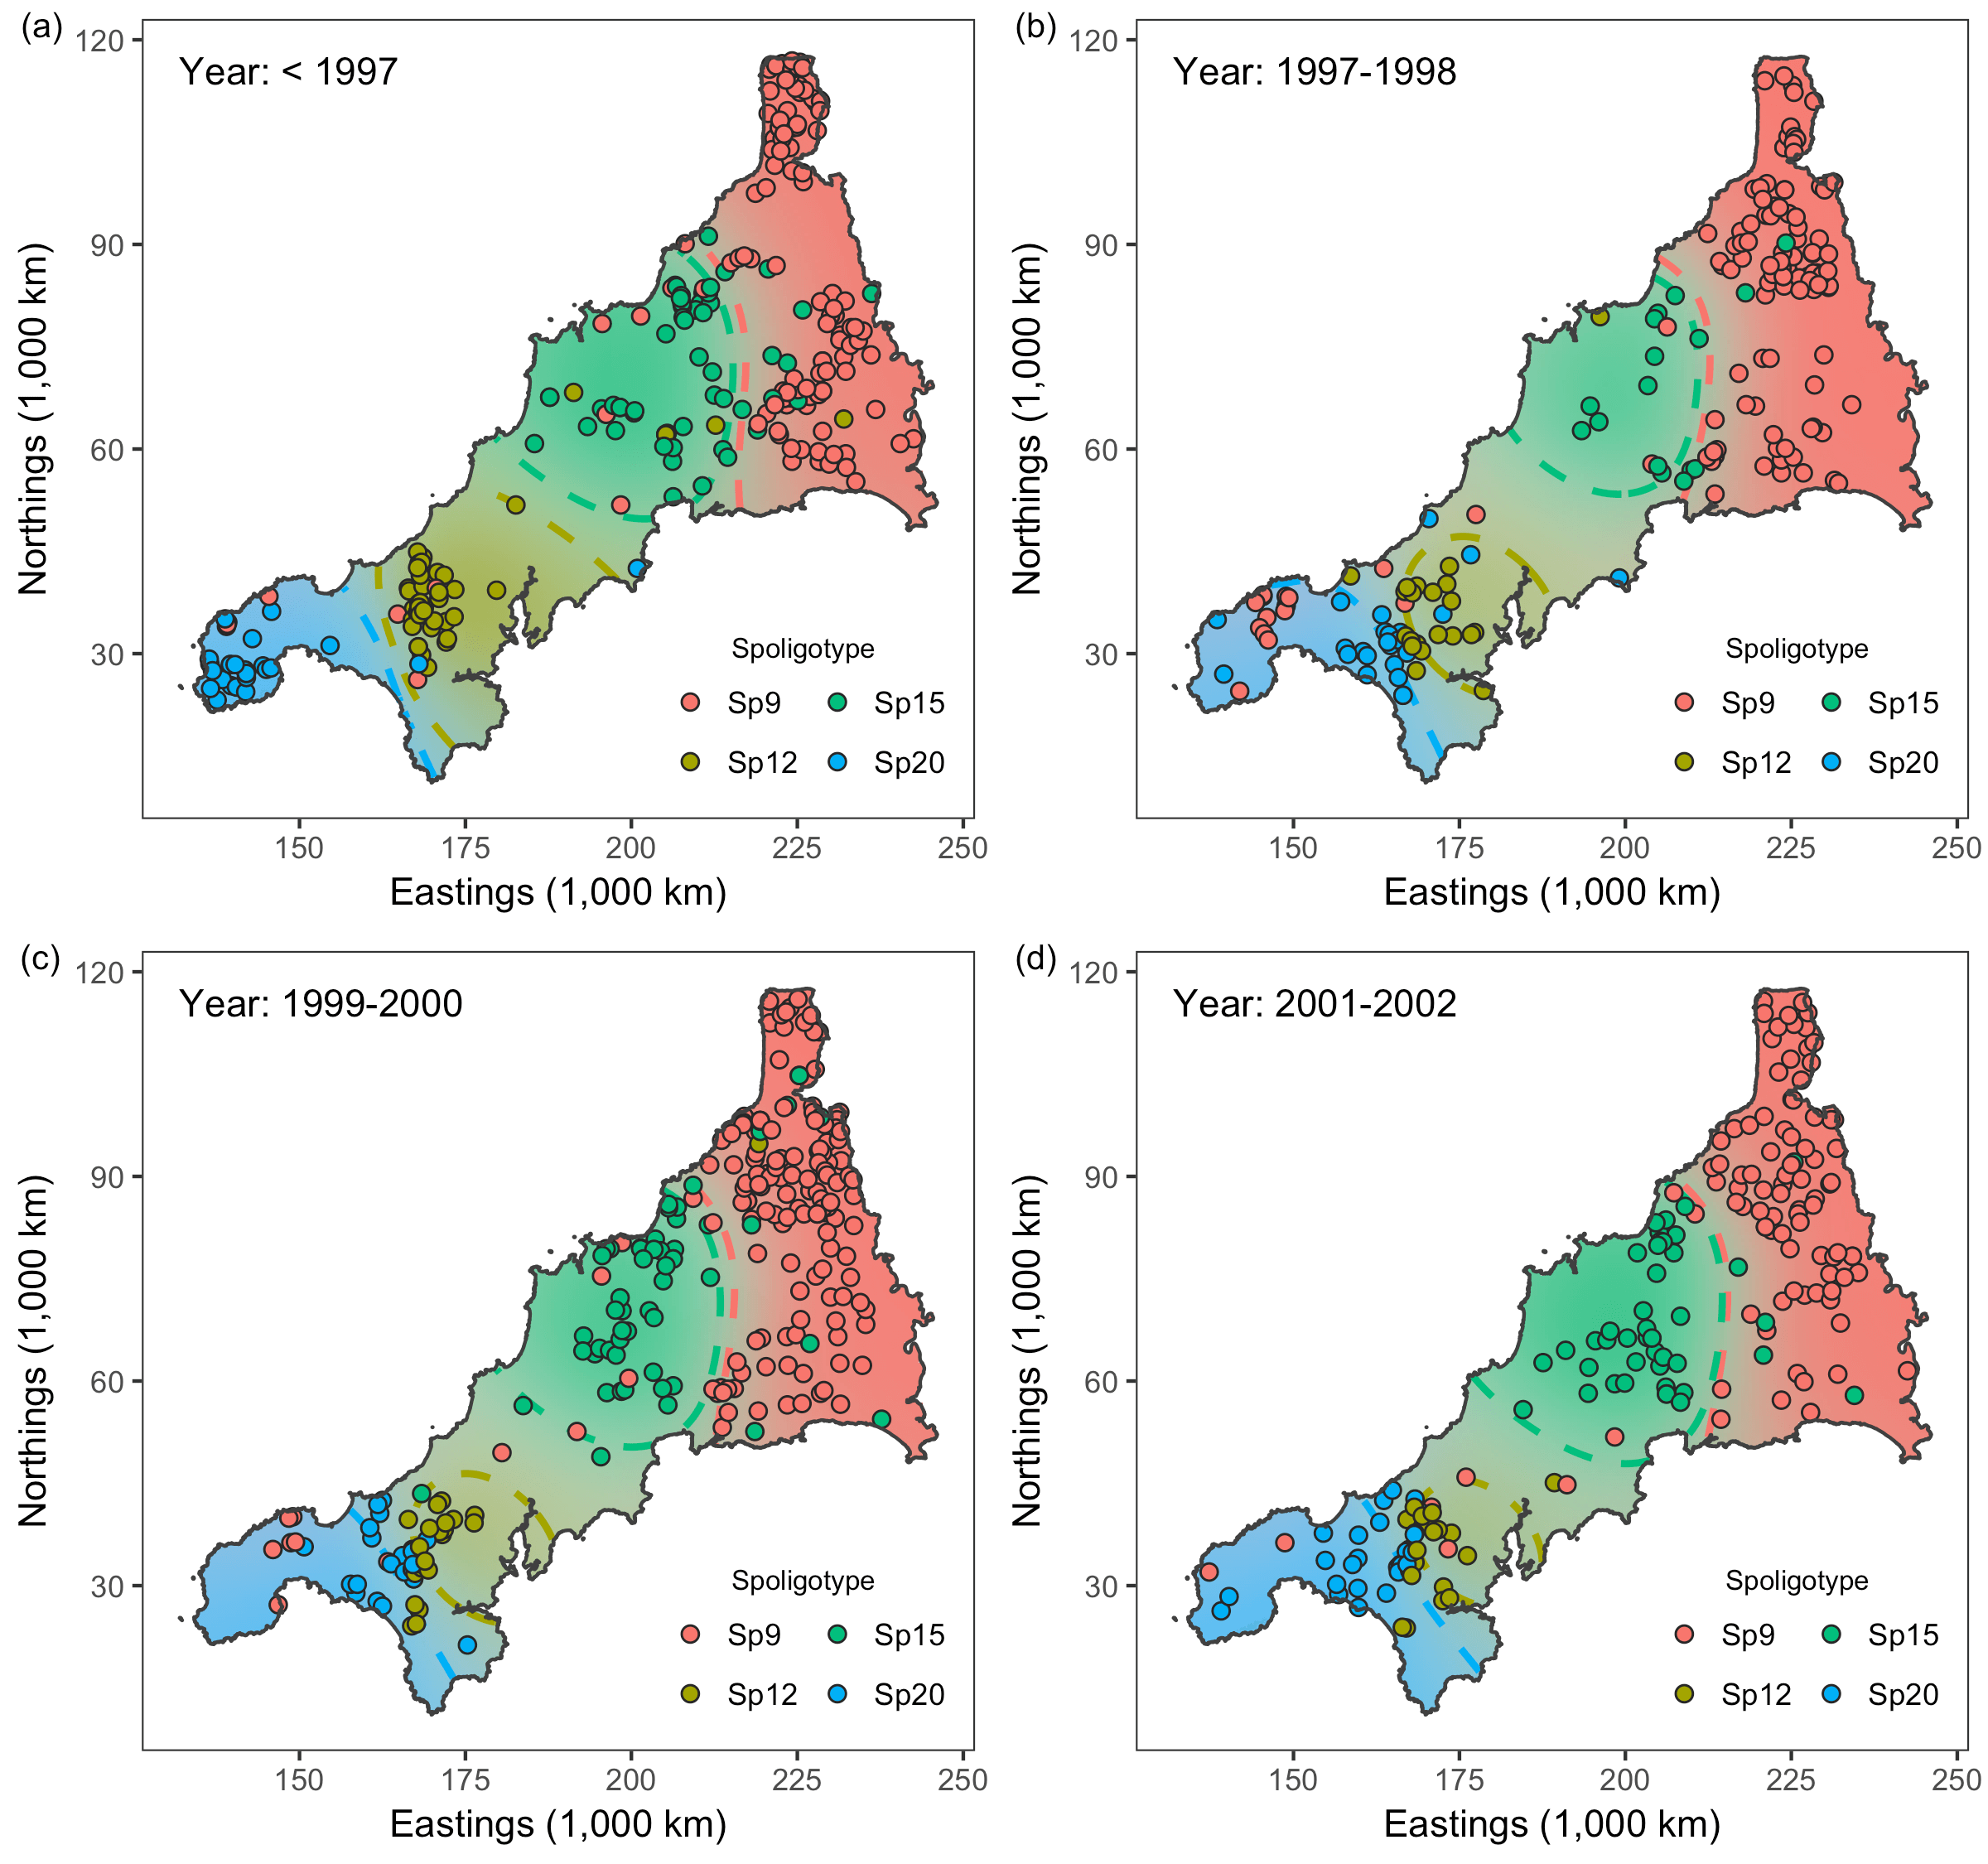
\includegraphics[width=\linewidth]{figure/05-plot_temporal_btb-1} 

}

\caption[Predicted probability surfaces for BTB contraction in Cornwall for the four largest spoligotypes of the bacterium \emph{Mycobacterium bovis} over four different time periods using model $M_3$]{Predicted probability surfaces for BTB contraction in Cornwall for the four largest spoligotypes of the bacterium \emph{Mycobacterium bovis} over four different time periods using model $M_3$.}\label{fig:plot.temporal.btb}
\end{figure}


\end{knitrout}

As the plots suggests, there is indeed spatial segregation for the four most common spoligotypes, and this is also very prominently seen from \cref{fig:plot.btb}.
In comparing the distribution of the spoligotypes over the years, we may refer to \cref{fig:plot.temporal.btb}, a series of predicted probability surface plots over the four time periods obtained from model $M_3$.
For each time period, we also superimposed the actual observations onto the predicted surface probabilities.
In addition, coloured dotted lines are displayed to indicate the ``decision boundaries'' for each of the four spoligotypes.
The most evident change is seen to the spatial distribution of spoligotype 12, with the decision boundary giving it a large area in years 1996 and earlier, but this steadily shrunk over the years.
Spoligotype 9, which is most commonly seen in the east of Cornwall, seems to have made its way down to the south-west over the years.
The other two spoligotypes seem to be rather constant over the years.

\end{document}




\section{Conclusion}
\label{sec:iprobitconcl}

This work presents an extension of the normal I-prior methodology to fit categorical response models using probit link functions---a methodology we call the I-probit.
The main motivation behind this work is to overcome the drawbacks of modelling probabilities using the normal I-prior model.
We assumed continuous latent variables that represent ``class propensities'' exist, which we modelled using normal I-priors, and transformed them into probabilities using a probit link function.
In this way, the advantages of the original I-prior methodology are preserved for categorical response models as well.

The core of this work explores ways in which to overcome the intractable integral presented by the I-probit model in \cref{eq:iprobitlik}.
Techniques such as quadrature methods, Laplace approximation and MCMC tend to fail, or are unsatisfactorily slow to accomplish.
The main reason for this is the dimension of this integral, which is $nm$, and thus for large sample sizes and/or number of classes, is unfeasible with such methods.
We turned to variational inference in the face of an intractable posterior density that hampers an EM algorithm, and the result is a sequential updating scheme, similar in time and storage requirements to the EM algorithm.

\index{additive model}
\index{Gausian process!classification}
\index{support vector machine}
\index{expectation propagation}
In terms of similarity to other works, the generalised additive models (GAMs) of \citet{hastie1986} comes close.
The setup of GAMs is near identical to the I-probit model, although estimation is done differently. 
GAMs do not assume smooth functions from any RKHS, but instead estimates the $f$'s using a local scoring method or a local likelihood method.
Kernel methods for classification are extremely popular in computer science and machine learning; examples include support vector machines \citep{scholkopf2002learning} and Gaussian process classification \citep{rasmussen2006gaussian}, with the latter being more closely related to the I-probit method.
However, Gaussian process classification typically uses the logistic sigmoid function, and estimation most commonly performed using Laplace approximation, but other methods such as expectation propagation \citep{minka2001expectation} and MCMC \citep{neal1999} have been explored as well.\index{logistic}
Variational inference for Gaussian process probit models have been studied by \citet{girolami2006variational}, with their work providing a close reference to the variational algorithm employed by us.

Suggestions for future work include:
\begin{enumerate}
  \item \textbf{Estimation of $\bPsi$}. 
  A limitation we had to face in this work was to treat $\bPsi$ as fixed.
  The discussion in \cref{sec:difficultPsi} shows that estimation of $\bPsi$ is possible, however, the specific nature of implementing this in computer code could not be explored in time.
  In particular, for the full I-probit model, the best method of imposing positive-definite constraints for $\bPsi$ in the M-step has not been fully researched.
  
  \item \textbf{Inclusion of class-specific covariates}. 
  Throughout the chapter, we assumed that covariates were unit-specific, rather than class-specific. 
  To illustrate, consider modelling the choice of travel mode between two destinations (car, coach, train or aeroplane) as a function of disposable income and travel time. 
  Individuals' income as a predictor of transportation choice is unit-specific, but clearly, travel time depends on the mode of transport. 
  To incorporate class-specific covariates $z_{ij}$, the regression on the latent propensities in \cref{eq:multinomial-latent} could be extended as such:
  \[
    y_{ij}^* = \myoverbrace{\alpha_j + f_j(x_i) + e(z_{ij})}{f(x_i,z_{ij},j)} + \epsilon_{ij}
  \]
  An I-prior would then be applied as usual, with careful consideration of the RKKS used to model $f$.
  
  \item \textbf{Improving computational efficiency}. 
  The $O(n^3m)$ time requirement for estimating I-probit models hinder its use towards large-data applications.
  In a limited study, we did not obtain reliable improvements using low-rank approximations of the kernel matrix such as the Nyström method.
  The key to improving computational efficiency could lie in sparse variational methods, a suggestion that was made to improve normal I-prior models as well.
\end{enumerate}

\begin{figure}[hbt]
  \centering
  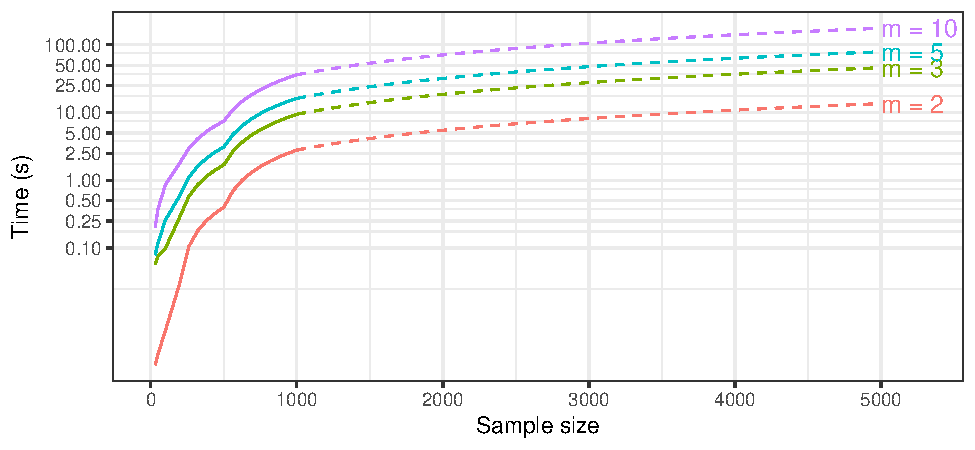
\includegraphics[width=0.9\textwidth]{figure/05-iprobit_runtime}
  \caption[Time taken to complete a single variational inference iteration]{Time taken to complete a single variational inference iteration for varying sample sizes and number of classes $m$. The solid line represents actual timings, while the dotted lines are linear extrapolations.}
\end{figure}

\index{variational Bayes}
As a final remark, we note that variational Bayes, which entails a fully Bayesian treatment of the model (setting priors on model parameters $\theta$), is a viable alternative to variational EM.
The output of such a variational inference algorithm would be approximate posterior densities for $\theta$, in addition to $q(\by^*)$ and $q(\bw)$, instead of point estimates for $\theta$.
Posterior inferences surrounding the parameters would then be possible, such as obtaining posterior standard deviations, credibility intervals, and so on.
However, a variational Bayes route has its cons:
\begin{enumerate}
  \item \textbf{Tedious derivations}. As the parameters now have a distribution $\theta = \{\balpha,\eta,\bPsi\} \sim q(\balpha,\eta,\bPsi)$, quantities such as
  \begin{itemize}
    \item $\E(\log \vert \bPsi \vert)$;
    \item $\E(\bH_\eta^2)$; and
    \item $\tr \E\big[ (\by^*-\bone_n\balpha^\top - \bH_\eta\bw)\bPsi (\by^*-\bone_n\balpha^\top - \bH_\eta\bw)^\top \big]$,
  \end{itemize}
  among others, will need to be derived for the variational inference algorithm, and these can be tricky to compute.
  
  \item \textbf{Suited only to conjugate exponential family models}. When conjugate exponential family models are considered, the approximate variational densities (under a mean-field assumption) are easily recognised, as they themselves belong to the same exponential family as the model or prior. However, I-prior does not always admit conjugacy for the kernel parameters $\eta$ (only for ANOVA RKKSs scale parameters), and most certainly not for $\bPsi$ (at least not in the current parameterisation). When this happens, techniques such as importance sampling or Metropolis algorithms need to be employed to obtain the posterior means required for the variational algorithm to proceed.
  
  \item \textbf{Prior specification and sensitivity}. It is not clear how best to specify prior information (from a subjectivist's standpoint) for the RKHS scale parameters, intercepts, and perhaps the error precision, because these are parameters relating to the latent propensities which are not very meaningful or interpretable. Of course, one could easily specify vague or even diffuse priors. The concern is that the model could be sensitive to prior choices.
\end{enumerate}

In consideration of the above, we opted to employ a variational EM algorithm for estimation of I-probit models, instead of a full variational Bayes estimation.
In any case, computational complexity is expected to be the same between the two methods.
An interesting point to note is that the RKHS scale parameters and intercept would admit a normal posterior under a variational Bayes scheme. 
This means that the posterior mode and the posterior mean coincide, so point estimates under a variational EM algorithm are exactly the same as the posterior mean estimates under a variational Bayes framework when a diffuse prior is used.

\hClosingStuffStandalone
\end{document}